\documentclass[12pt,a4paper,titlepage]{article}

\usepackage{preamble}

\title{Transformée discrête en ondelettes : travaux pratiques}
\author{Yassine Jamoud, Samy Haffoudhi}
\date{\today}

\begin{document}

\maketitle

\section*{Introduction}

Le but de ce TP est de prendre en main la transformée en ondelettes à l'aide de Matlab et de
la boîte à outils \texttt{Wavelab}. Nous allons alors commencer par tracer des fonctions ondelettes,
échelles et une transformée en ondelettes. Nous implémenterons ensuite une procédure de
"débruitage" basée sur la transformée en ondelettes et enfin nous réaliserons de la compression
d'images.

\section{Tracé d'ondelettes et de fonctions échelles par DWT inverse}

\begin{enumerate}

    \item{Sous forme informatique la DWT est représentée sous la forme :
            $$ \texttt{DWT}(x) = [a_J, d_J, d_{J-1}, \dots, d_1] $$ où $J$ est l'échelle maximale.

            Ainsi, $\forall j, k$,

            \begin{itemize}
                \item{Le coefficient $a_J[k]$ est à l'indice k dans la représentation.}
                \item{Le coefficient $d_j[k]$ est à l'indice $ \frac{N}{2^j} + k  $}
            \end{itemize}
        }

    \item{ On souhaite construire un vecteur \texttt{DWT x} contenant seulement un coefficient non-nul
            de détail à la plus grande échelle et situé approximativement au milieu de l'axe temporel.

            On place alors d'après 1. ce coefficient non-nul à l'indice :
            $ \frac{N}{2^J} + \frac{N}{2^{J+1}} = \frac{3N}{2^{J+1}} $

        \item{Traçons alors l'allure de la fonction ondelette correspondant à la transformée de
                Haar :

                \begin{figure}[H]
                    \caption{Fonction ondelette (Haar)}
                    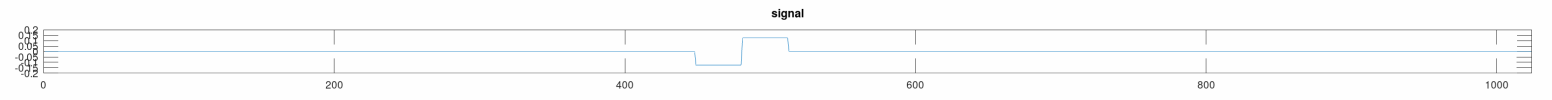
\includegraphics[width=\textwidth]{ex1_1}
                    \centering
                \end{figure}
            }

        \item{Représentons les fonctions échelles correspondantes :

                \begin{figure}[H]
                    \caption{Fonctions échelles (Haar)}
                    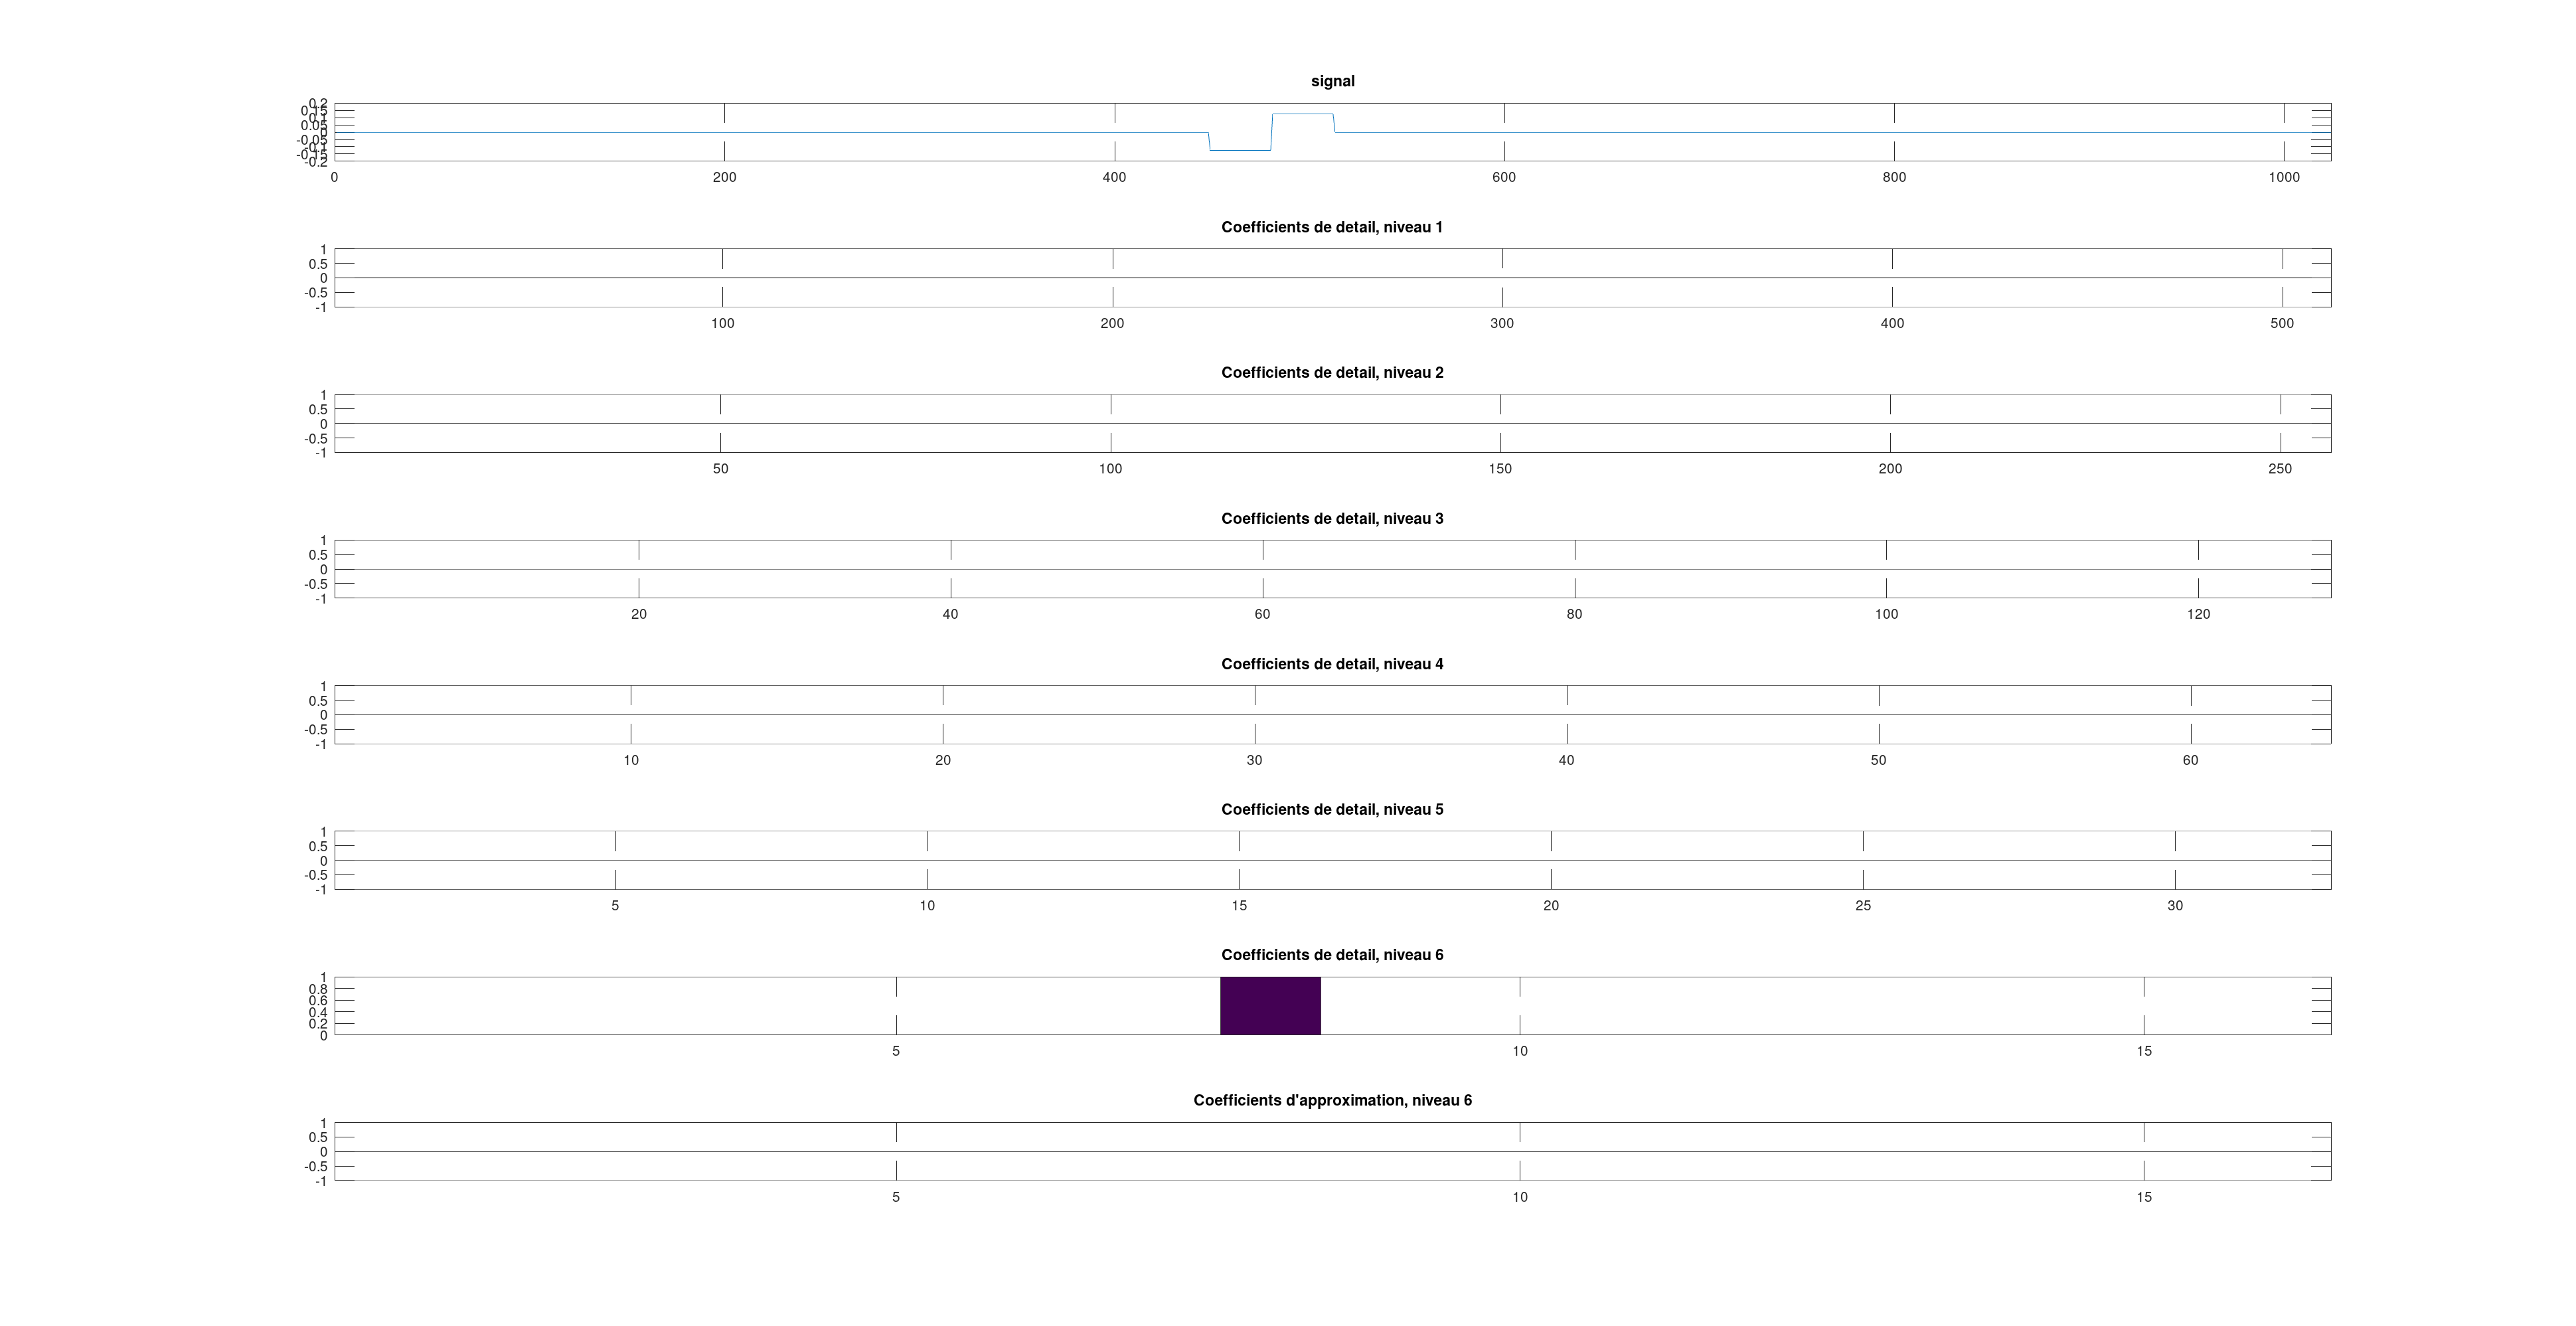
\includegraphics[width=\textwidth]{ex1_2}
                    \centering
                \end{figure}
            }

        \setcounter{enumi}{5}

        \item{Répétons la procédure pour les ondelettes de Daubechies d'ordre 4 et 8 :

                \begin{figure}[H]
                    \caption{Fonction ondelette (Daubechies d'ordre 4)}
                    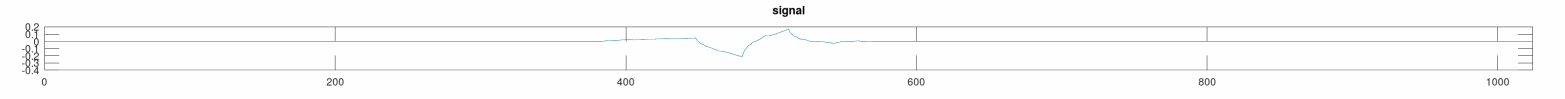
\includegraphics[width=\textwidth]{ex1_3}
                    \centering
                \end{figure}

                \begin{figure}[H]
                    \caption{Fonctions échelles (Daubechies d'ordre 4)}
                    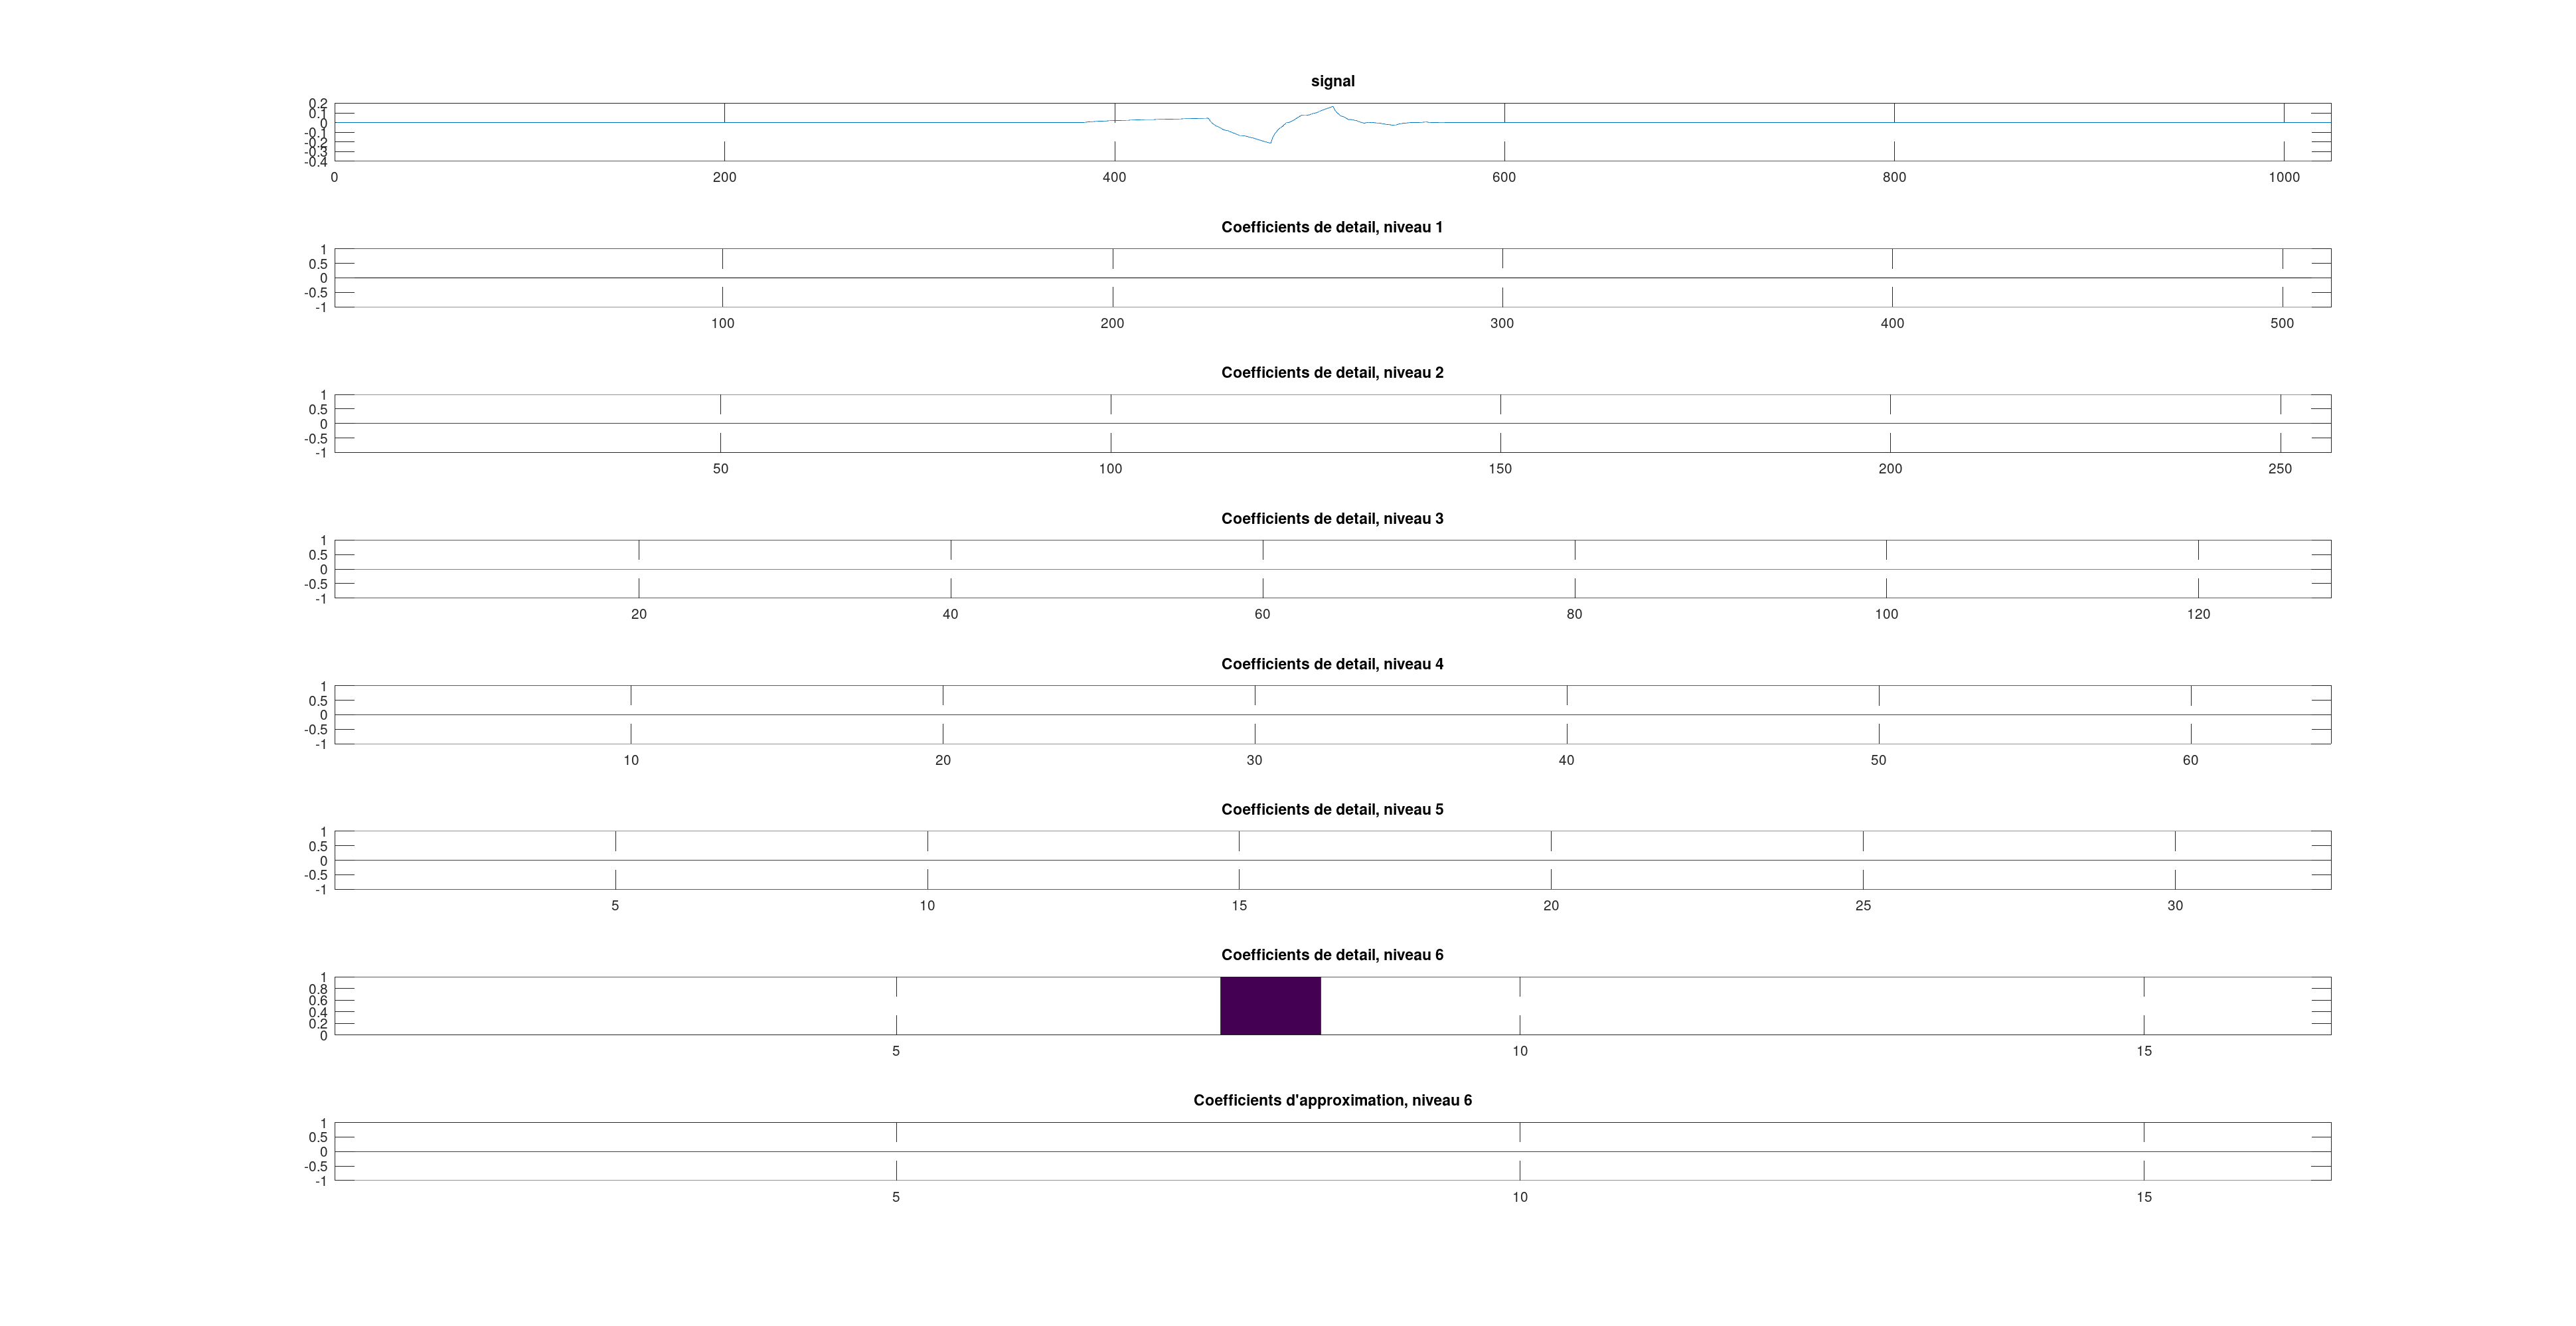
\includegraphics[width=\textwidth]{ex1_4}
                    \centering
                \end{figure}

                \begin{figure}[H]
                    \caption{Fonction ondelette (Daubechies d'ordre 8)}
                    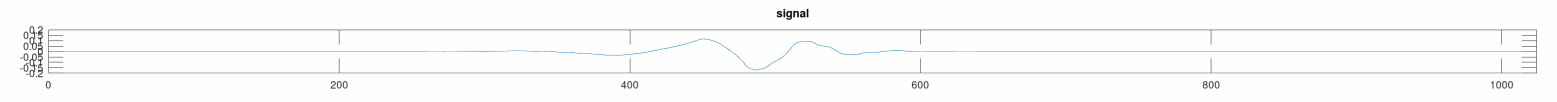
\includegraphics[width=\textwidth]{ex1_5}
                    \centering
                \end{figure}

                \begin{figure}[H]
                    \caption{Fonctions échelles (Daubechies d'ordre 8)}
                    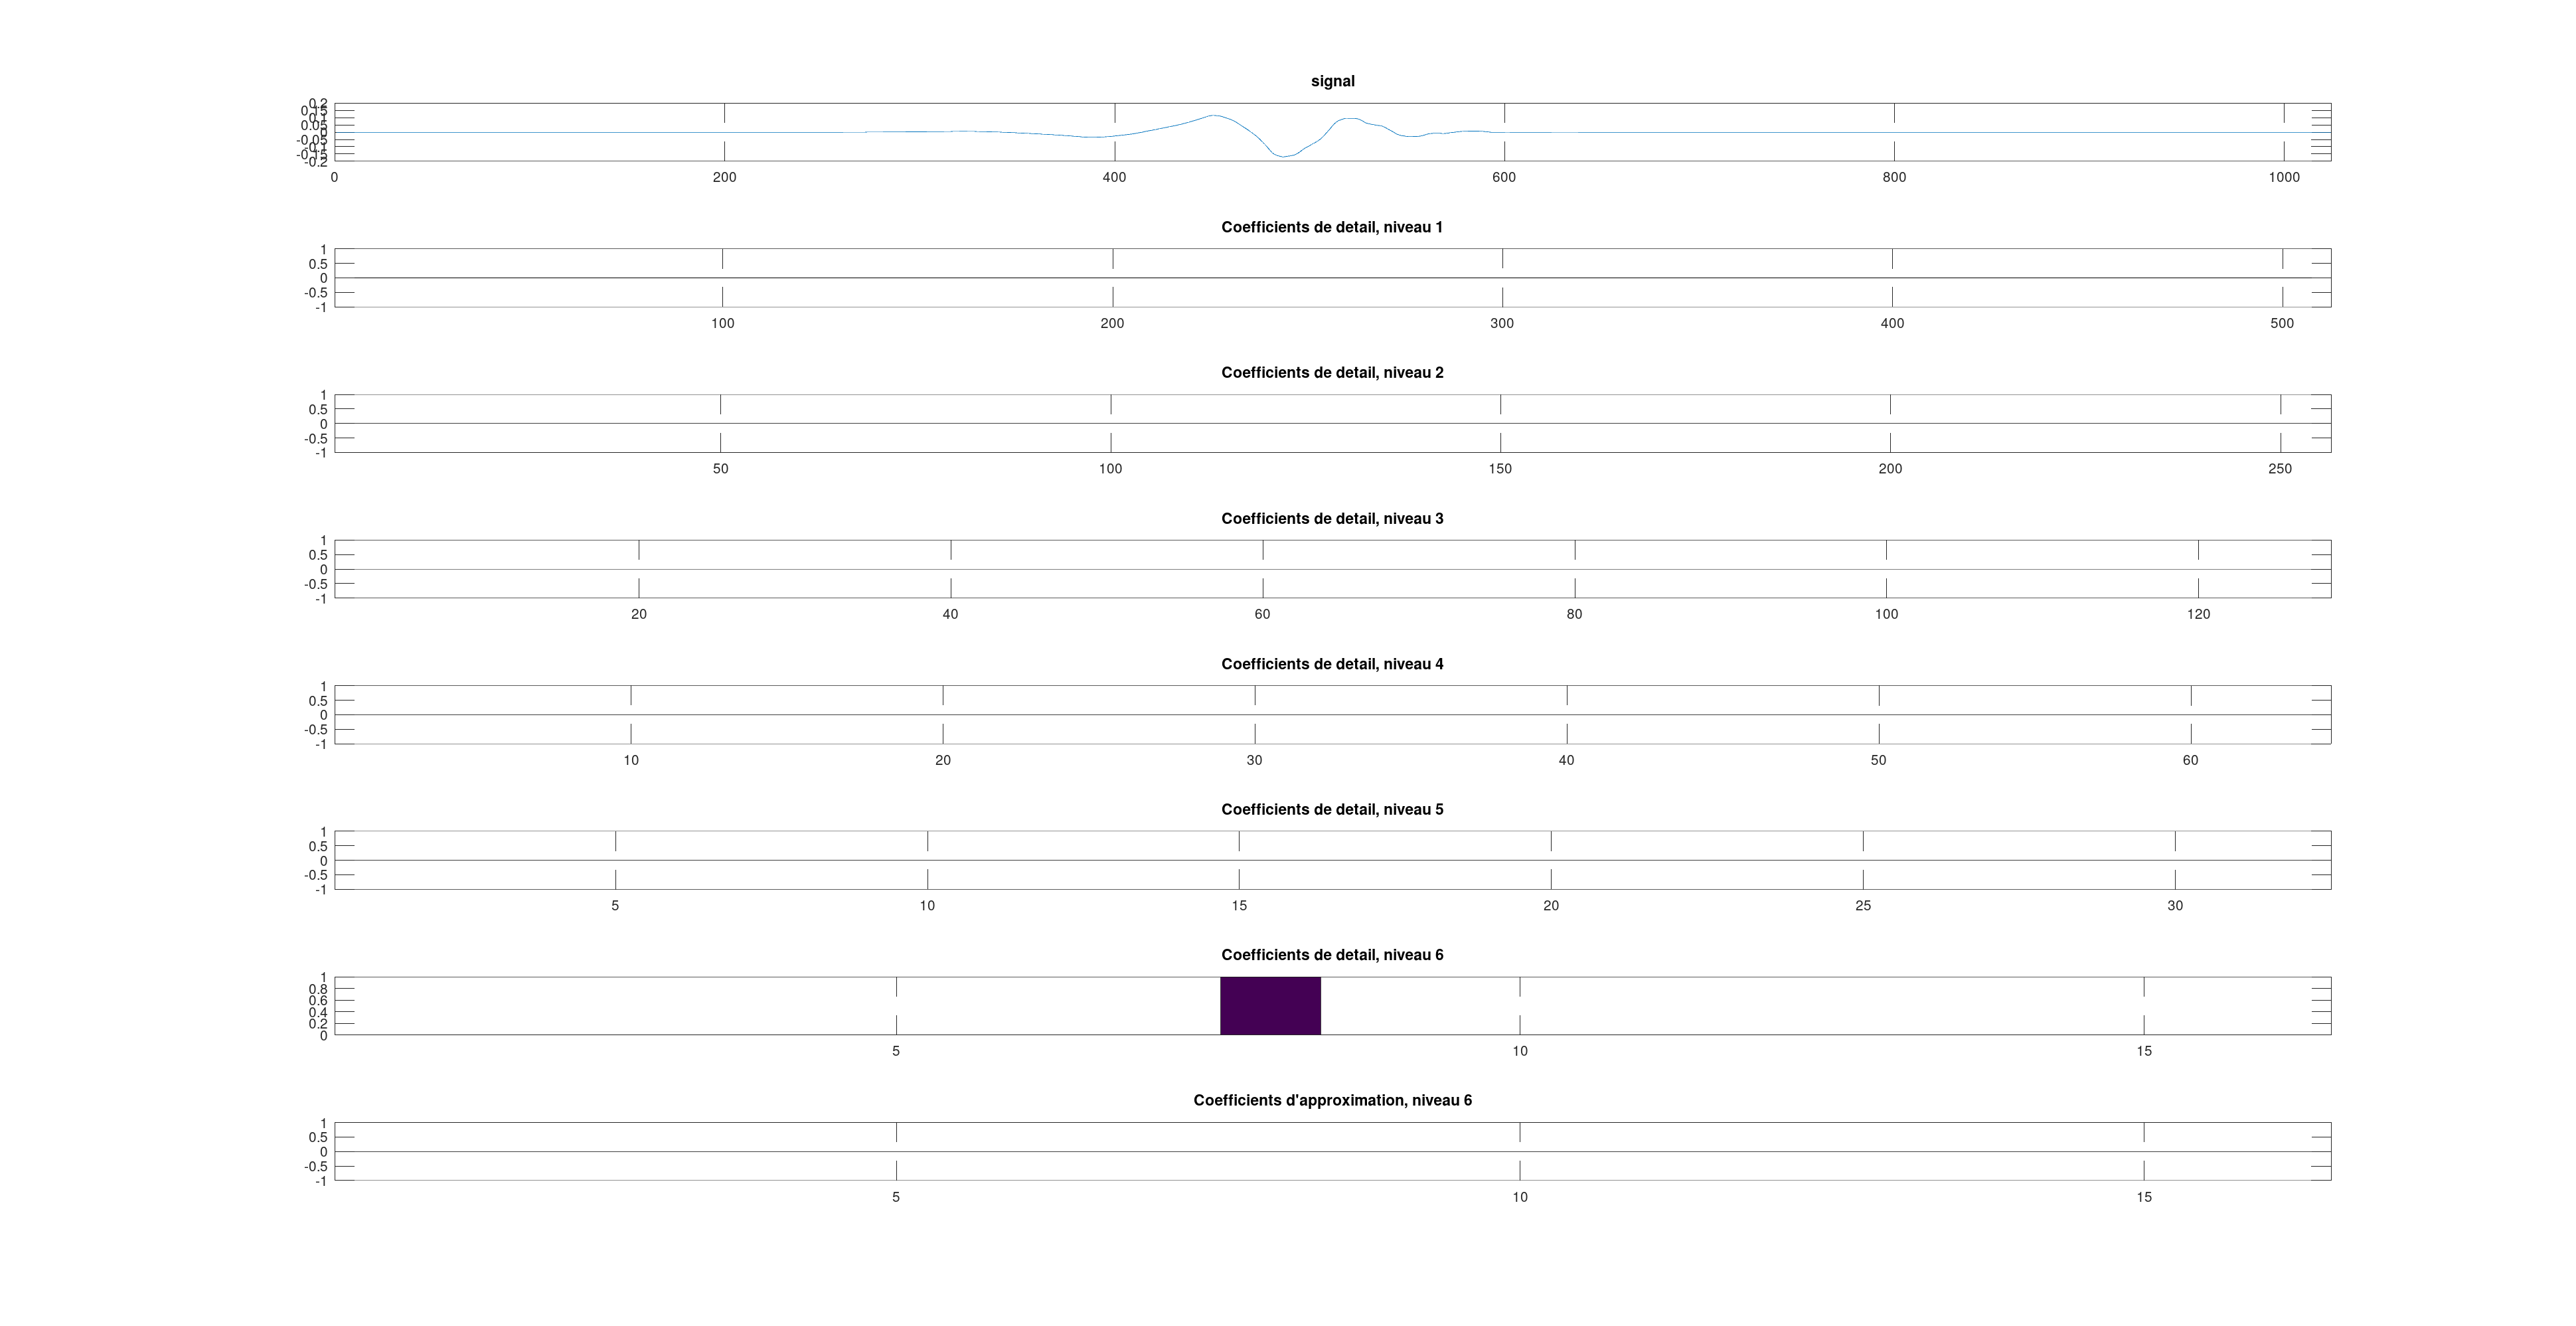
\includegraphics[width=\textwidth]{ex1_6}
                    \centering
                \end{figure}

            }

        \item{Ainsi, d'après les tracés précédents, la fonction ondelette correspondant à la
            transformée de Haar est constante par morceaux, celles de Daubechies sont plus
        complexes mais on retrouve les formes vues en cours, on note notamment la présence des
    pics.}

    \end{enumerate}

    \section{Débruitage dans l'espace des ondelettes}

    \emph{On considèrera dans toute cette partie une ondelette de Haar.}

    \begin{enumerate}
        \item{Créons un signal dont la DWT jusqu'à l'échelle  J = 7 contient
                uniquement quelques coefficients de détail non nuls.

                Représentons alors le signal obtenu et sa DWT :

                \begin{figure}[H]
                    \caption{Signal}
                    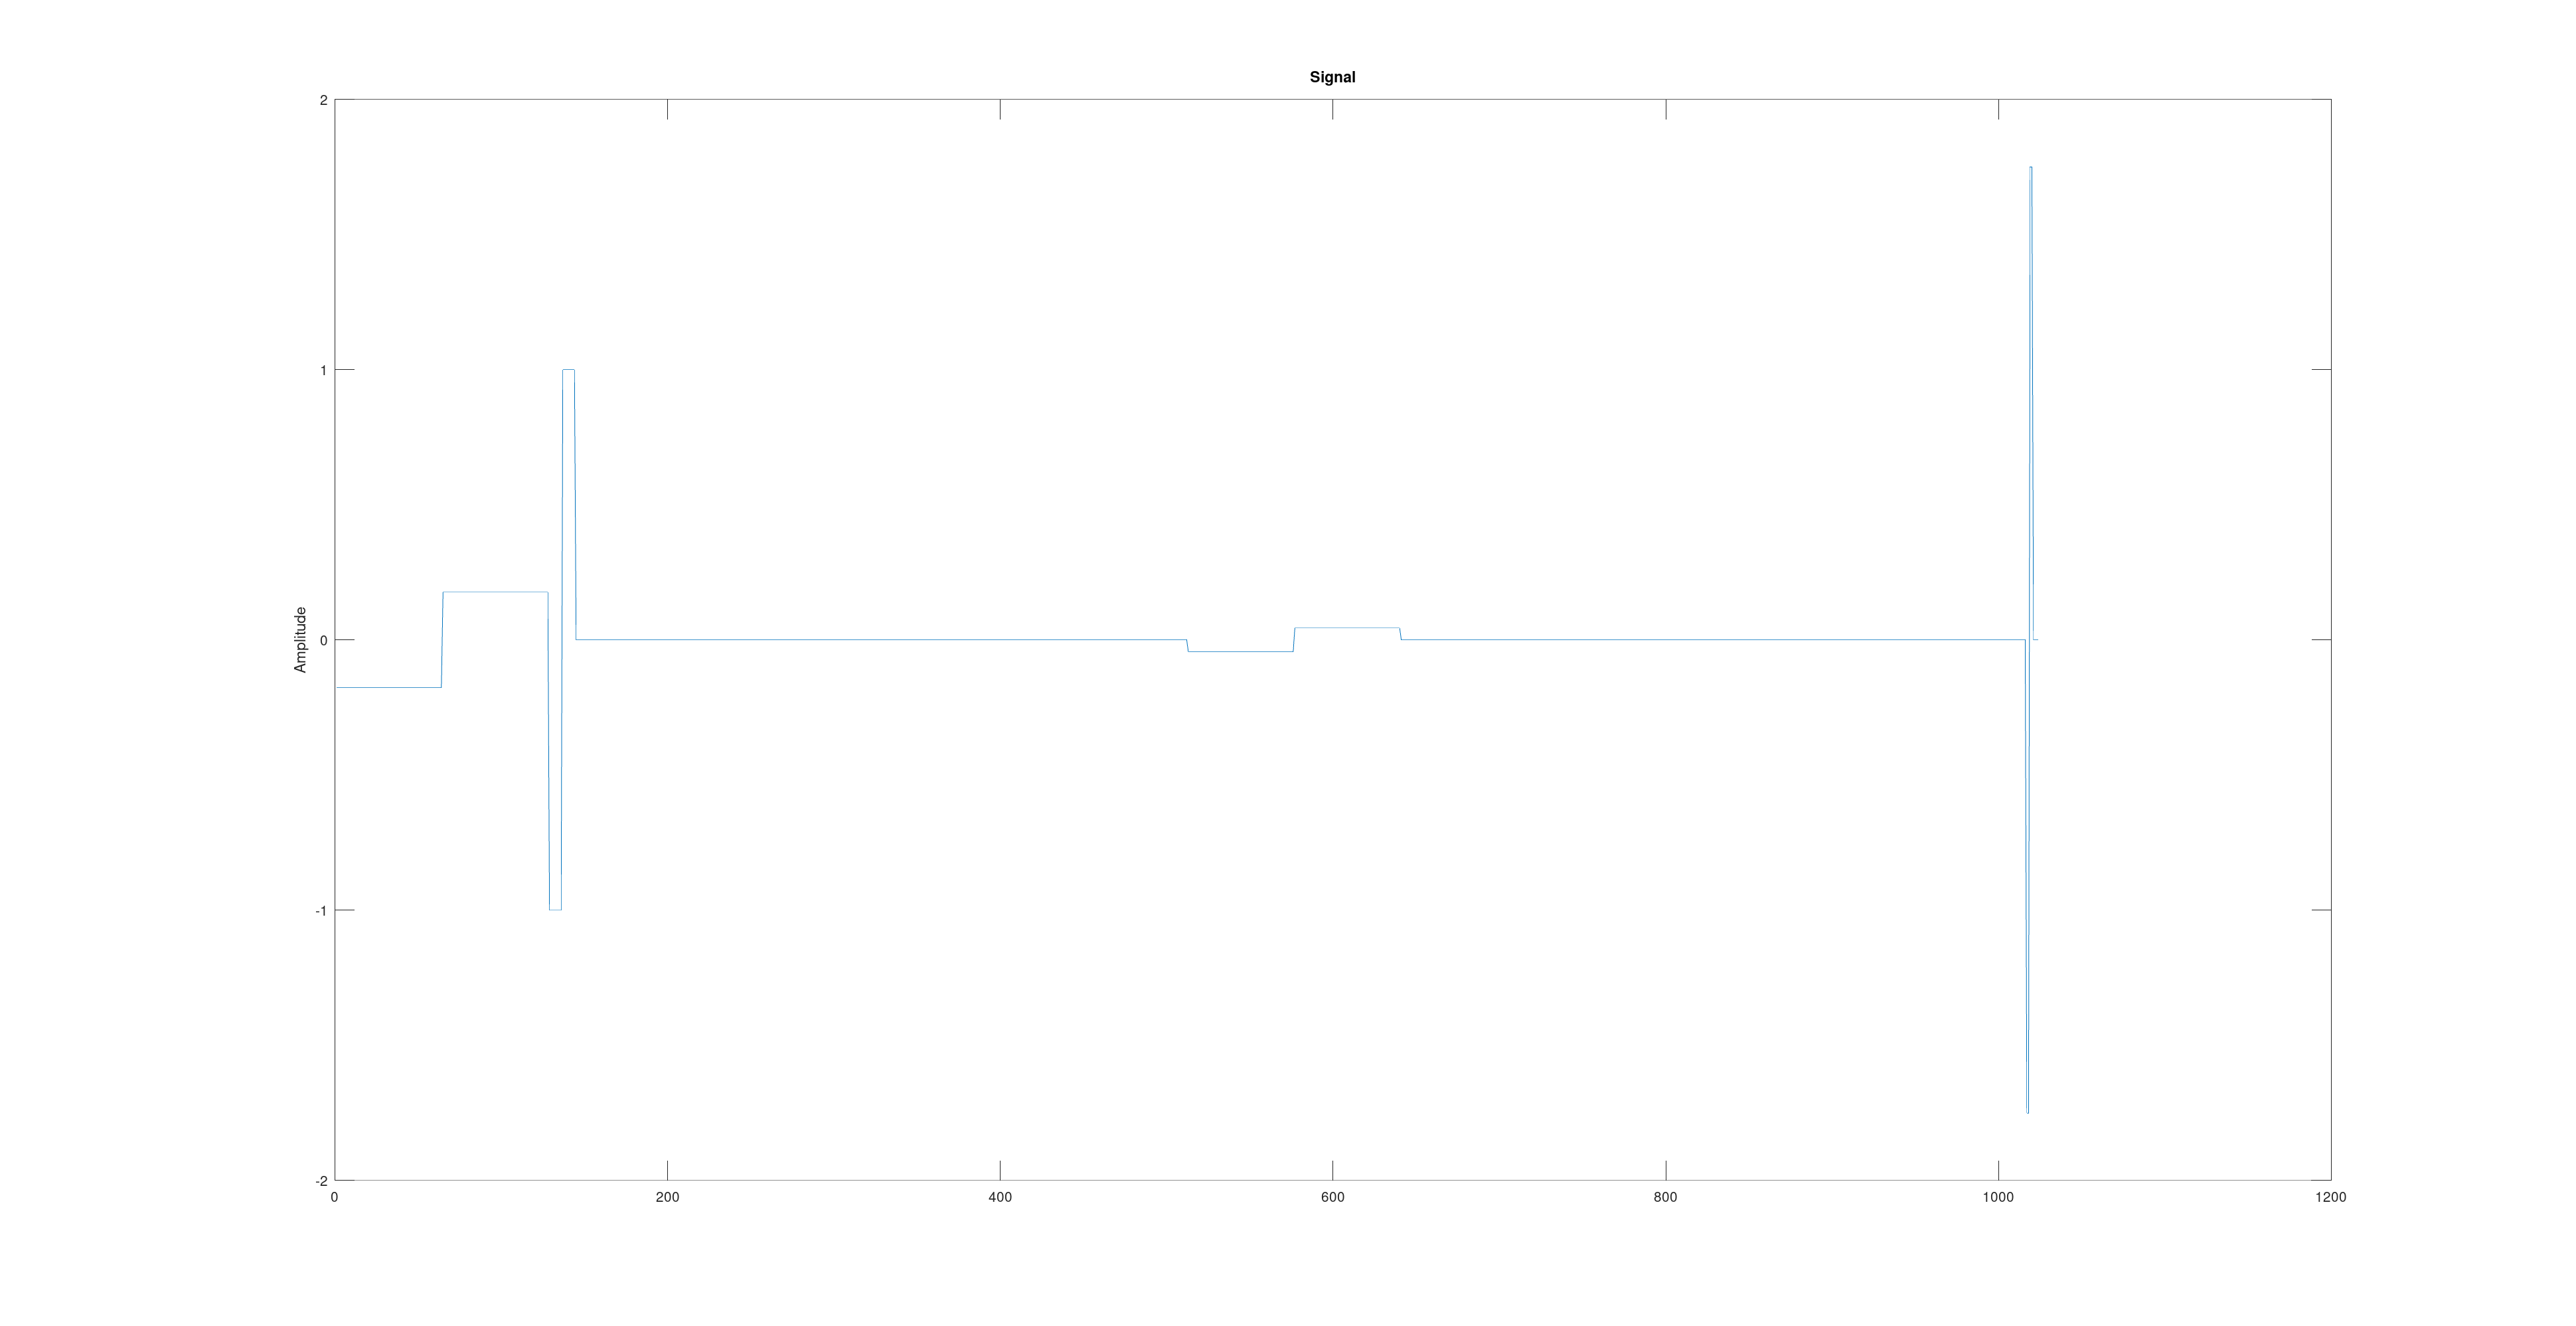
\includegraphics[width=\textwidth]{ex2_1_bis}
                    \centering
                \end{figure}

                \begin{figure}[H]
                    \caption{DWT du signal}
                    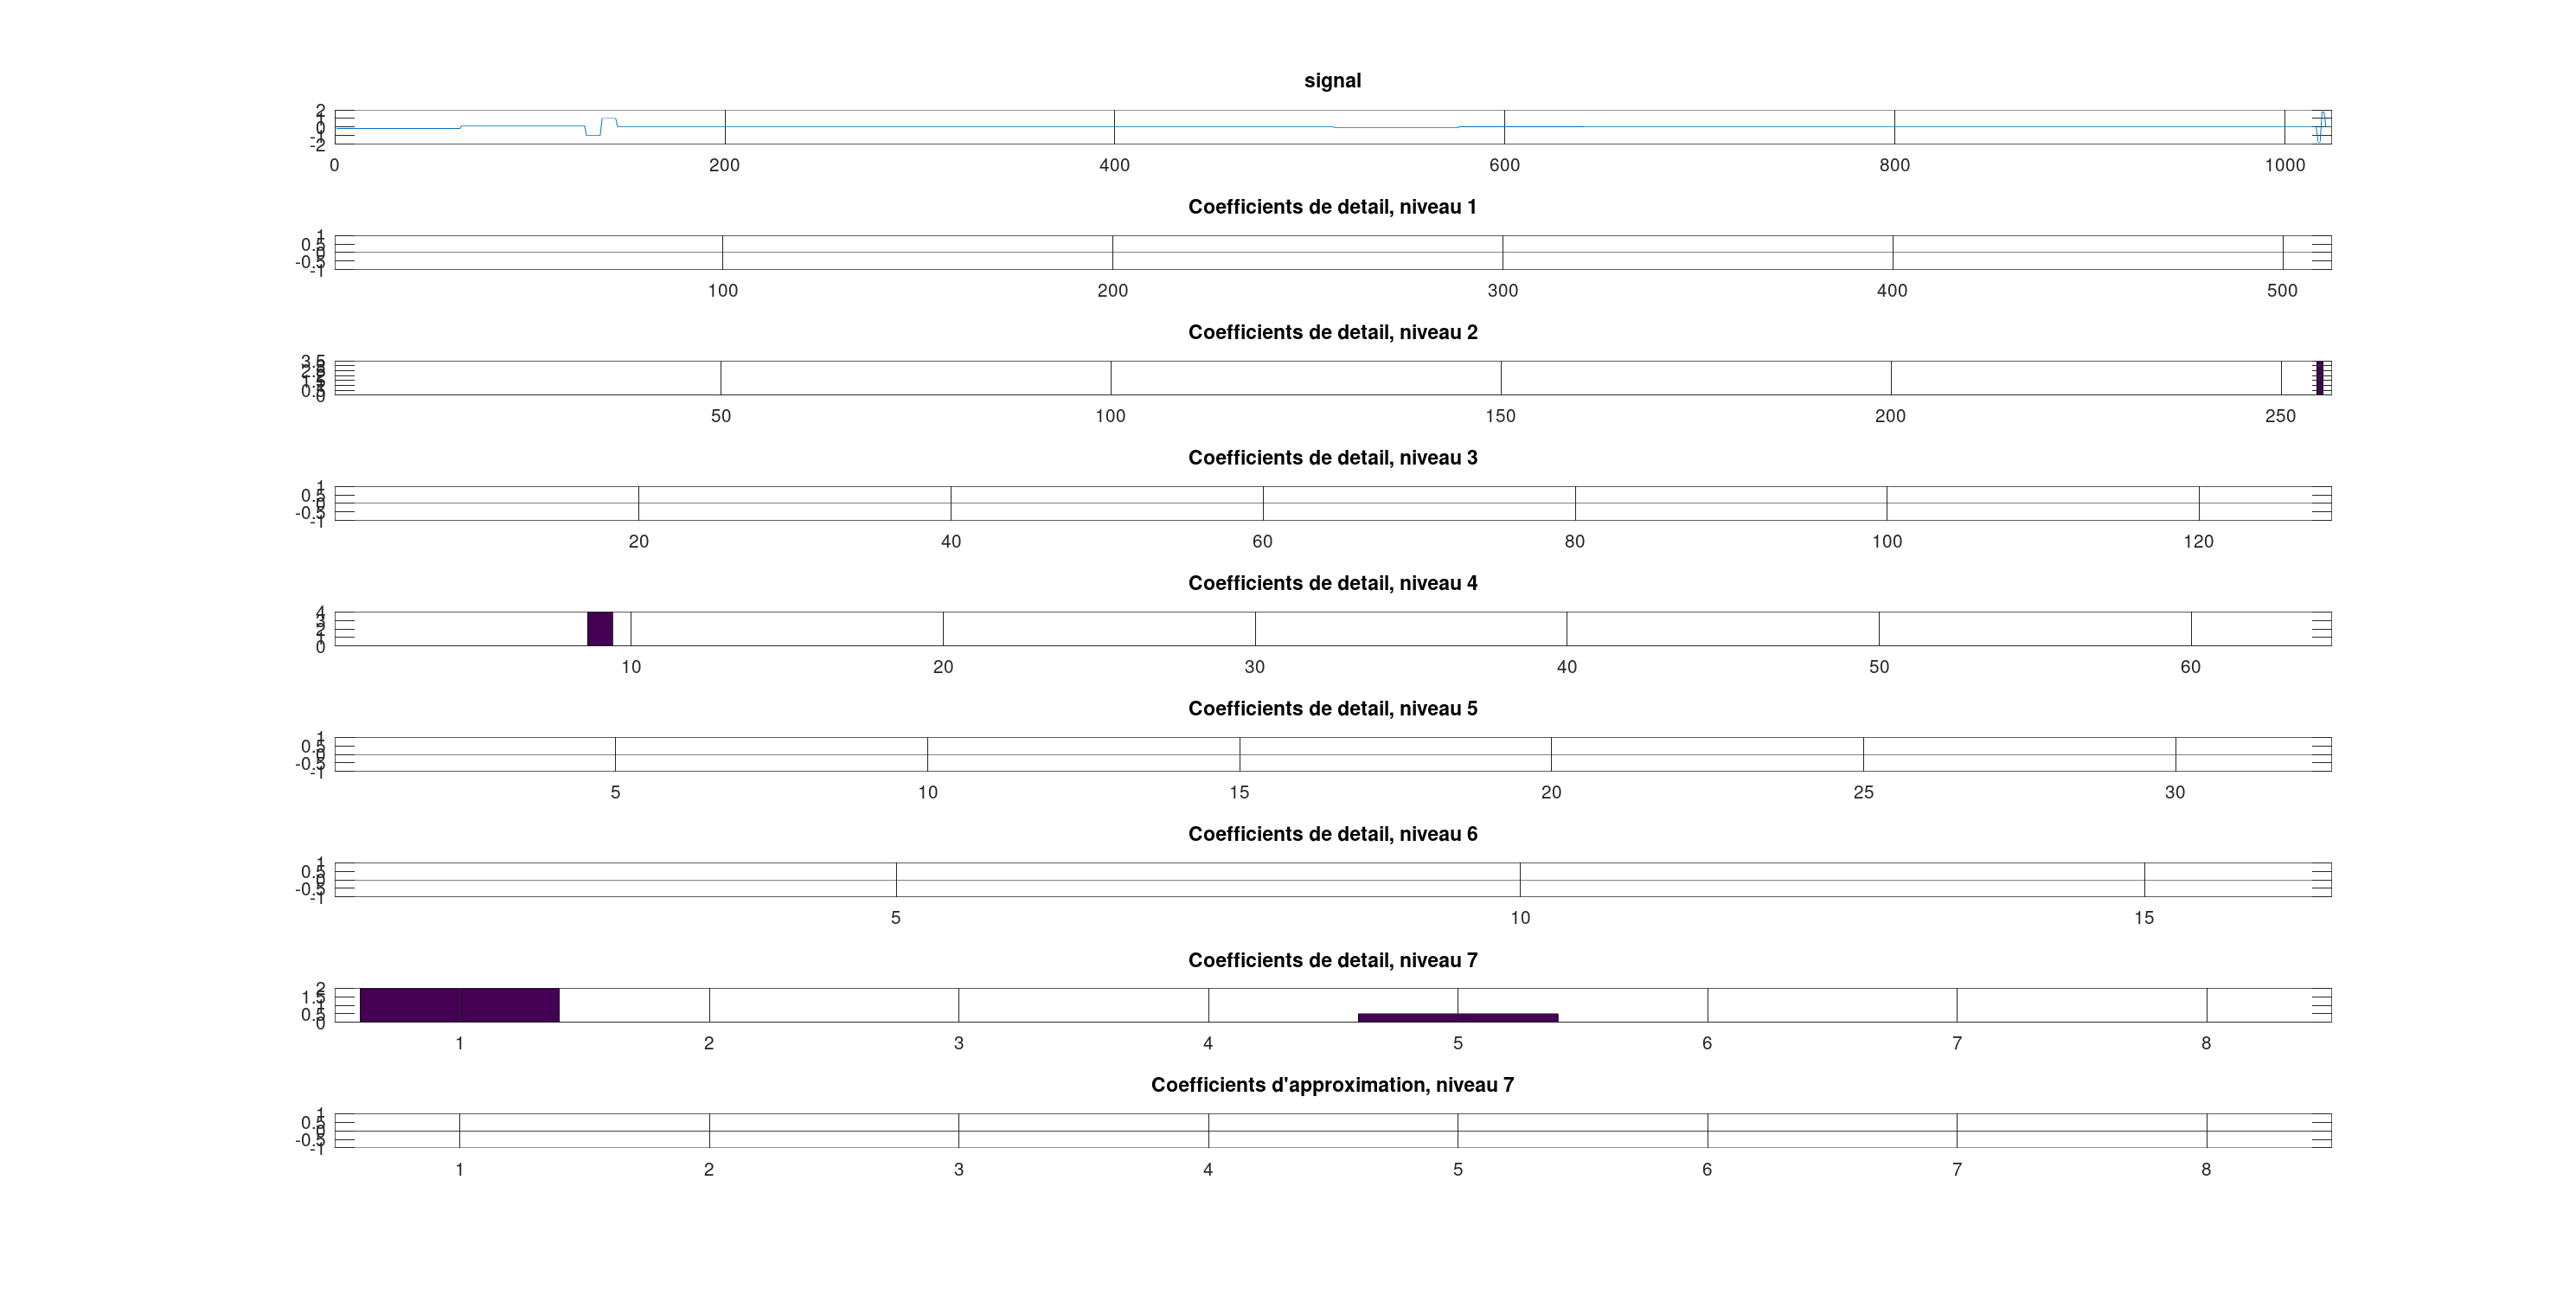
\includegraphics[width=\textwidth]{ex2_1}
                    \centering
                \end{figure}
            }

        \item{Ajoutons du bruit au signal obtenu et visualisons ce nouveau
                signal ainsi que sa DWT :

                \begin{figure}[H]
                    \caption{Signal bruité}
                    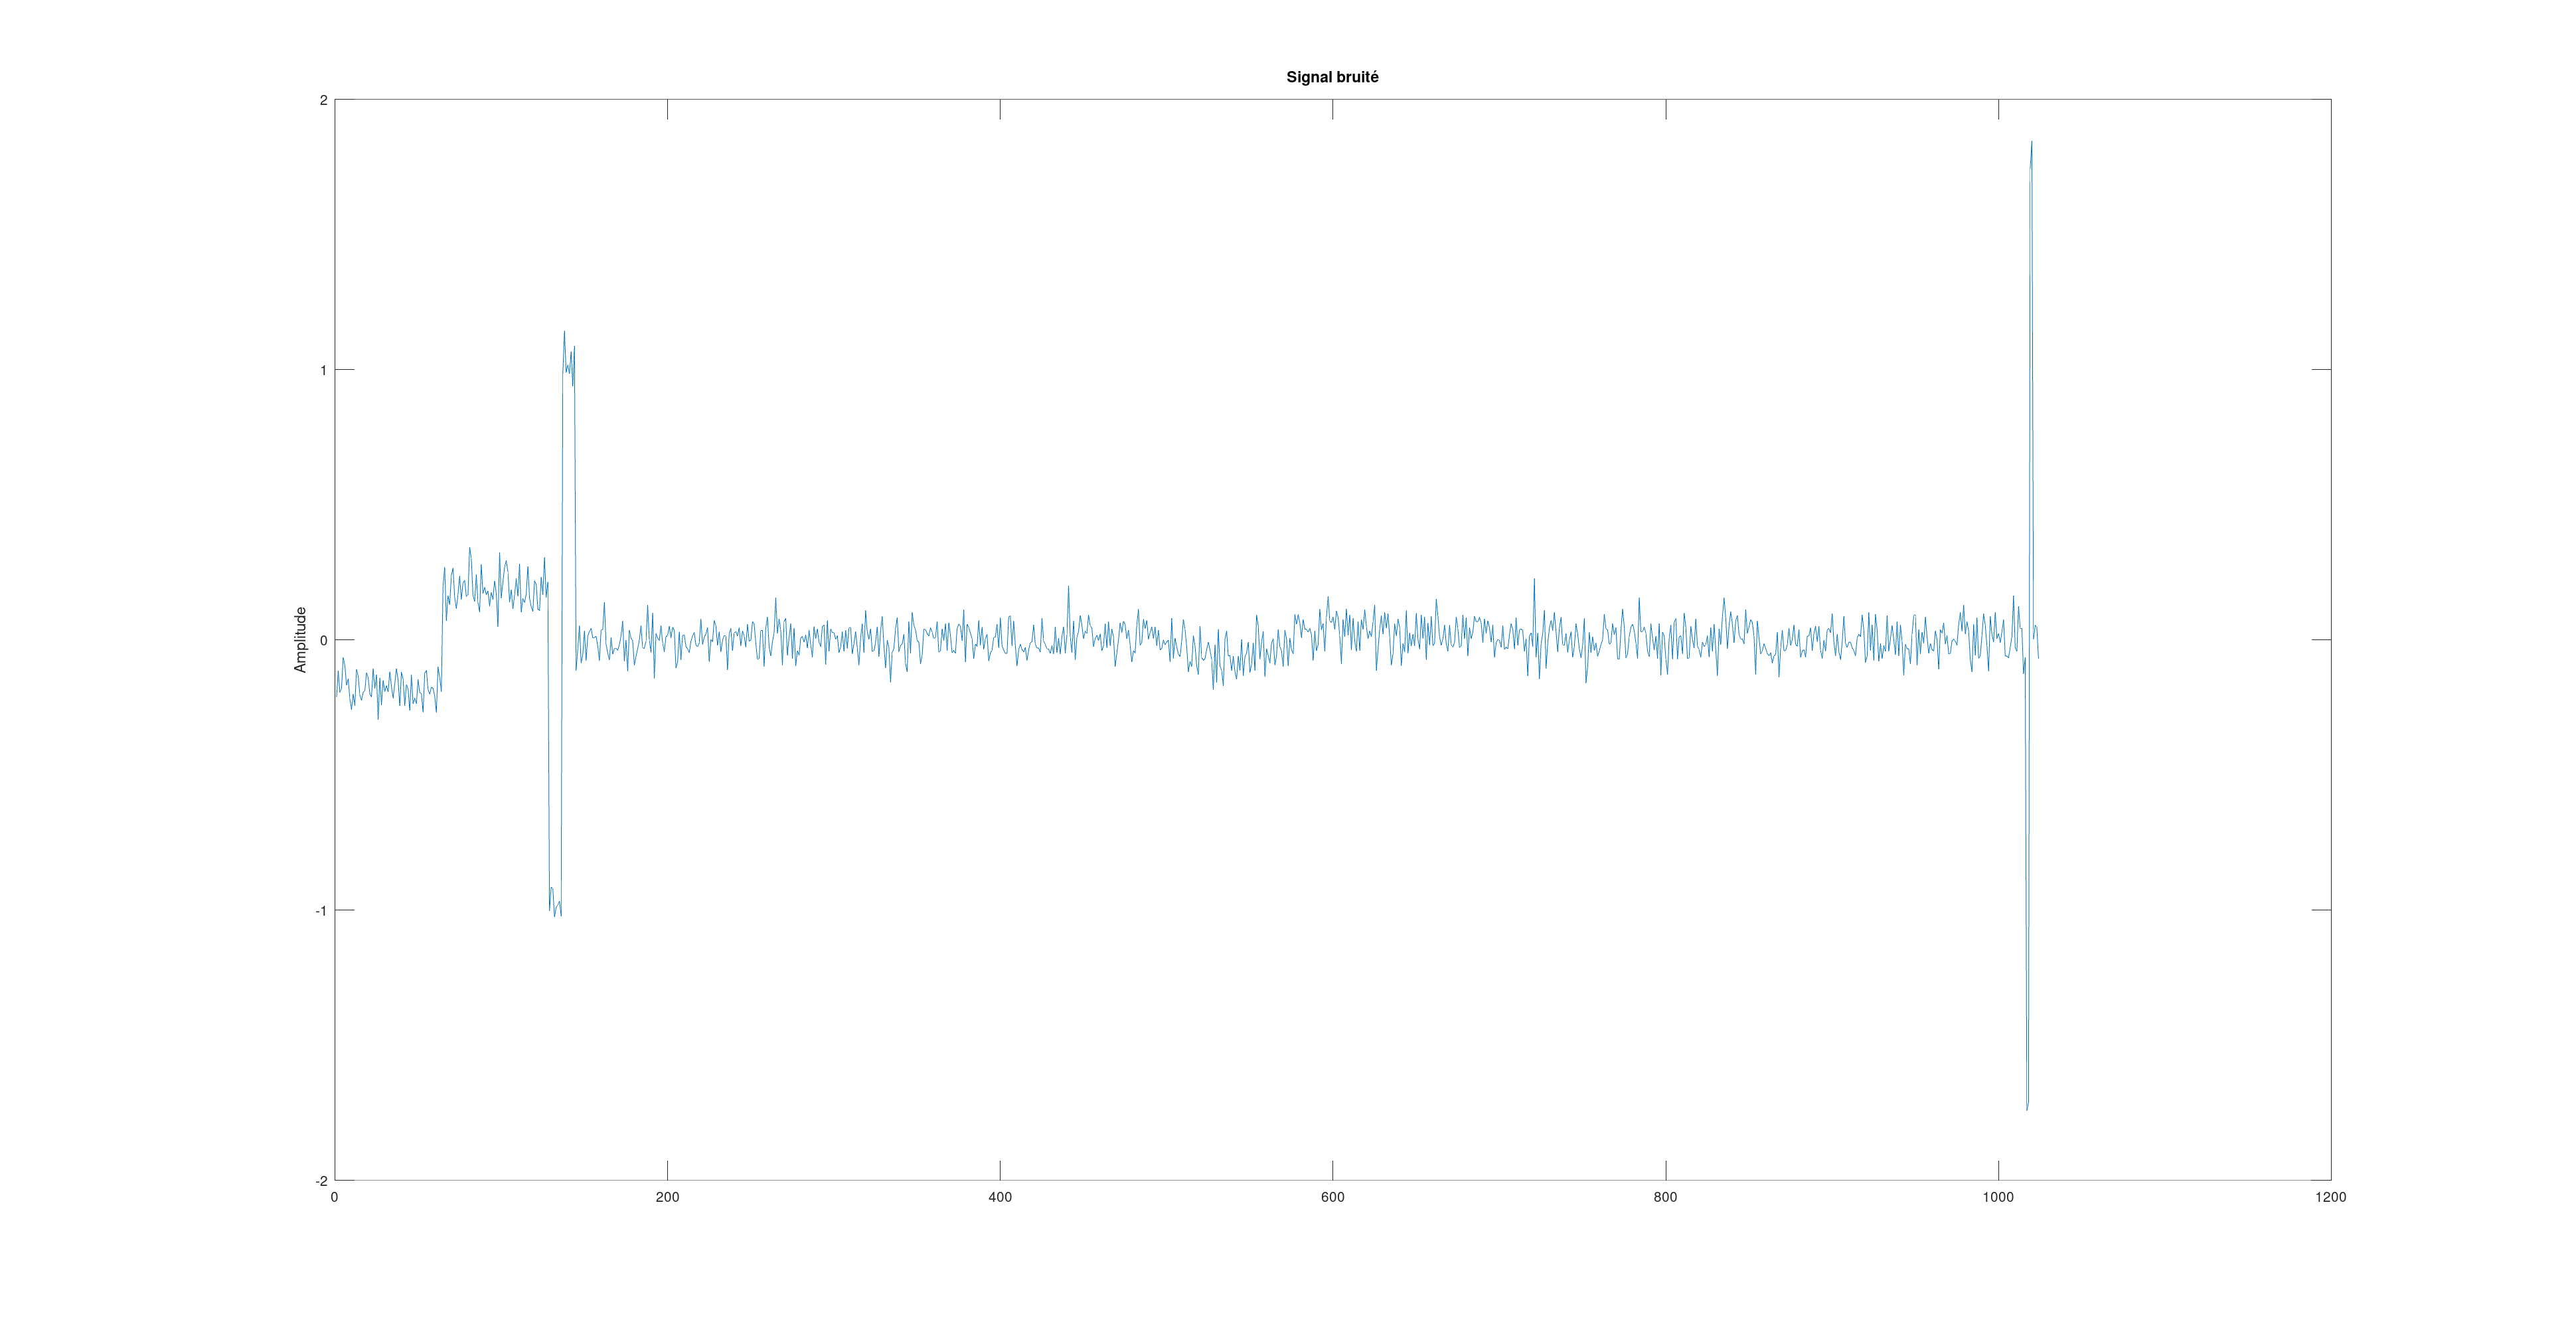
\includegraphics[width=\textwidth]{ex2_2_bis}
                    \centering
                \end{figure}

                \begin{figure}[H]
                    \caption{DWT du signal bruité}
                    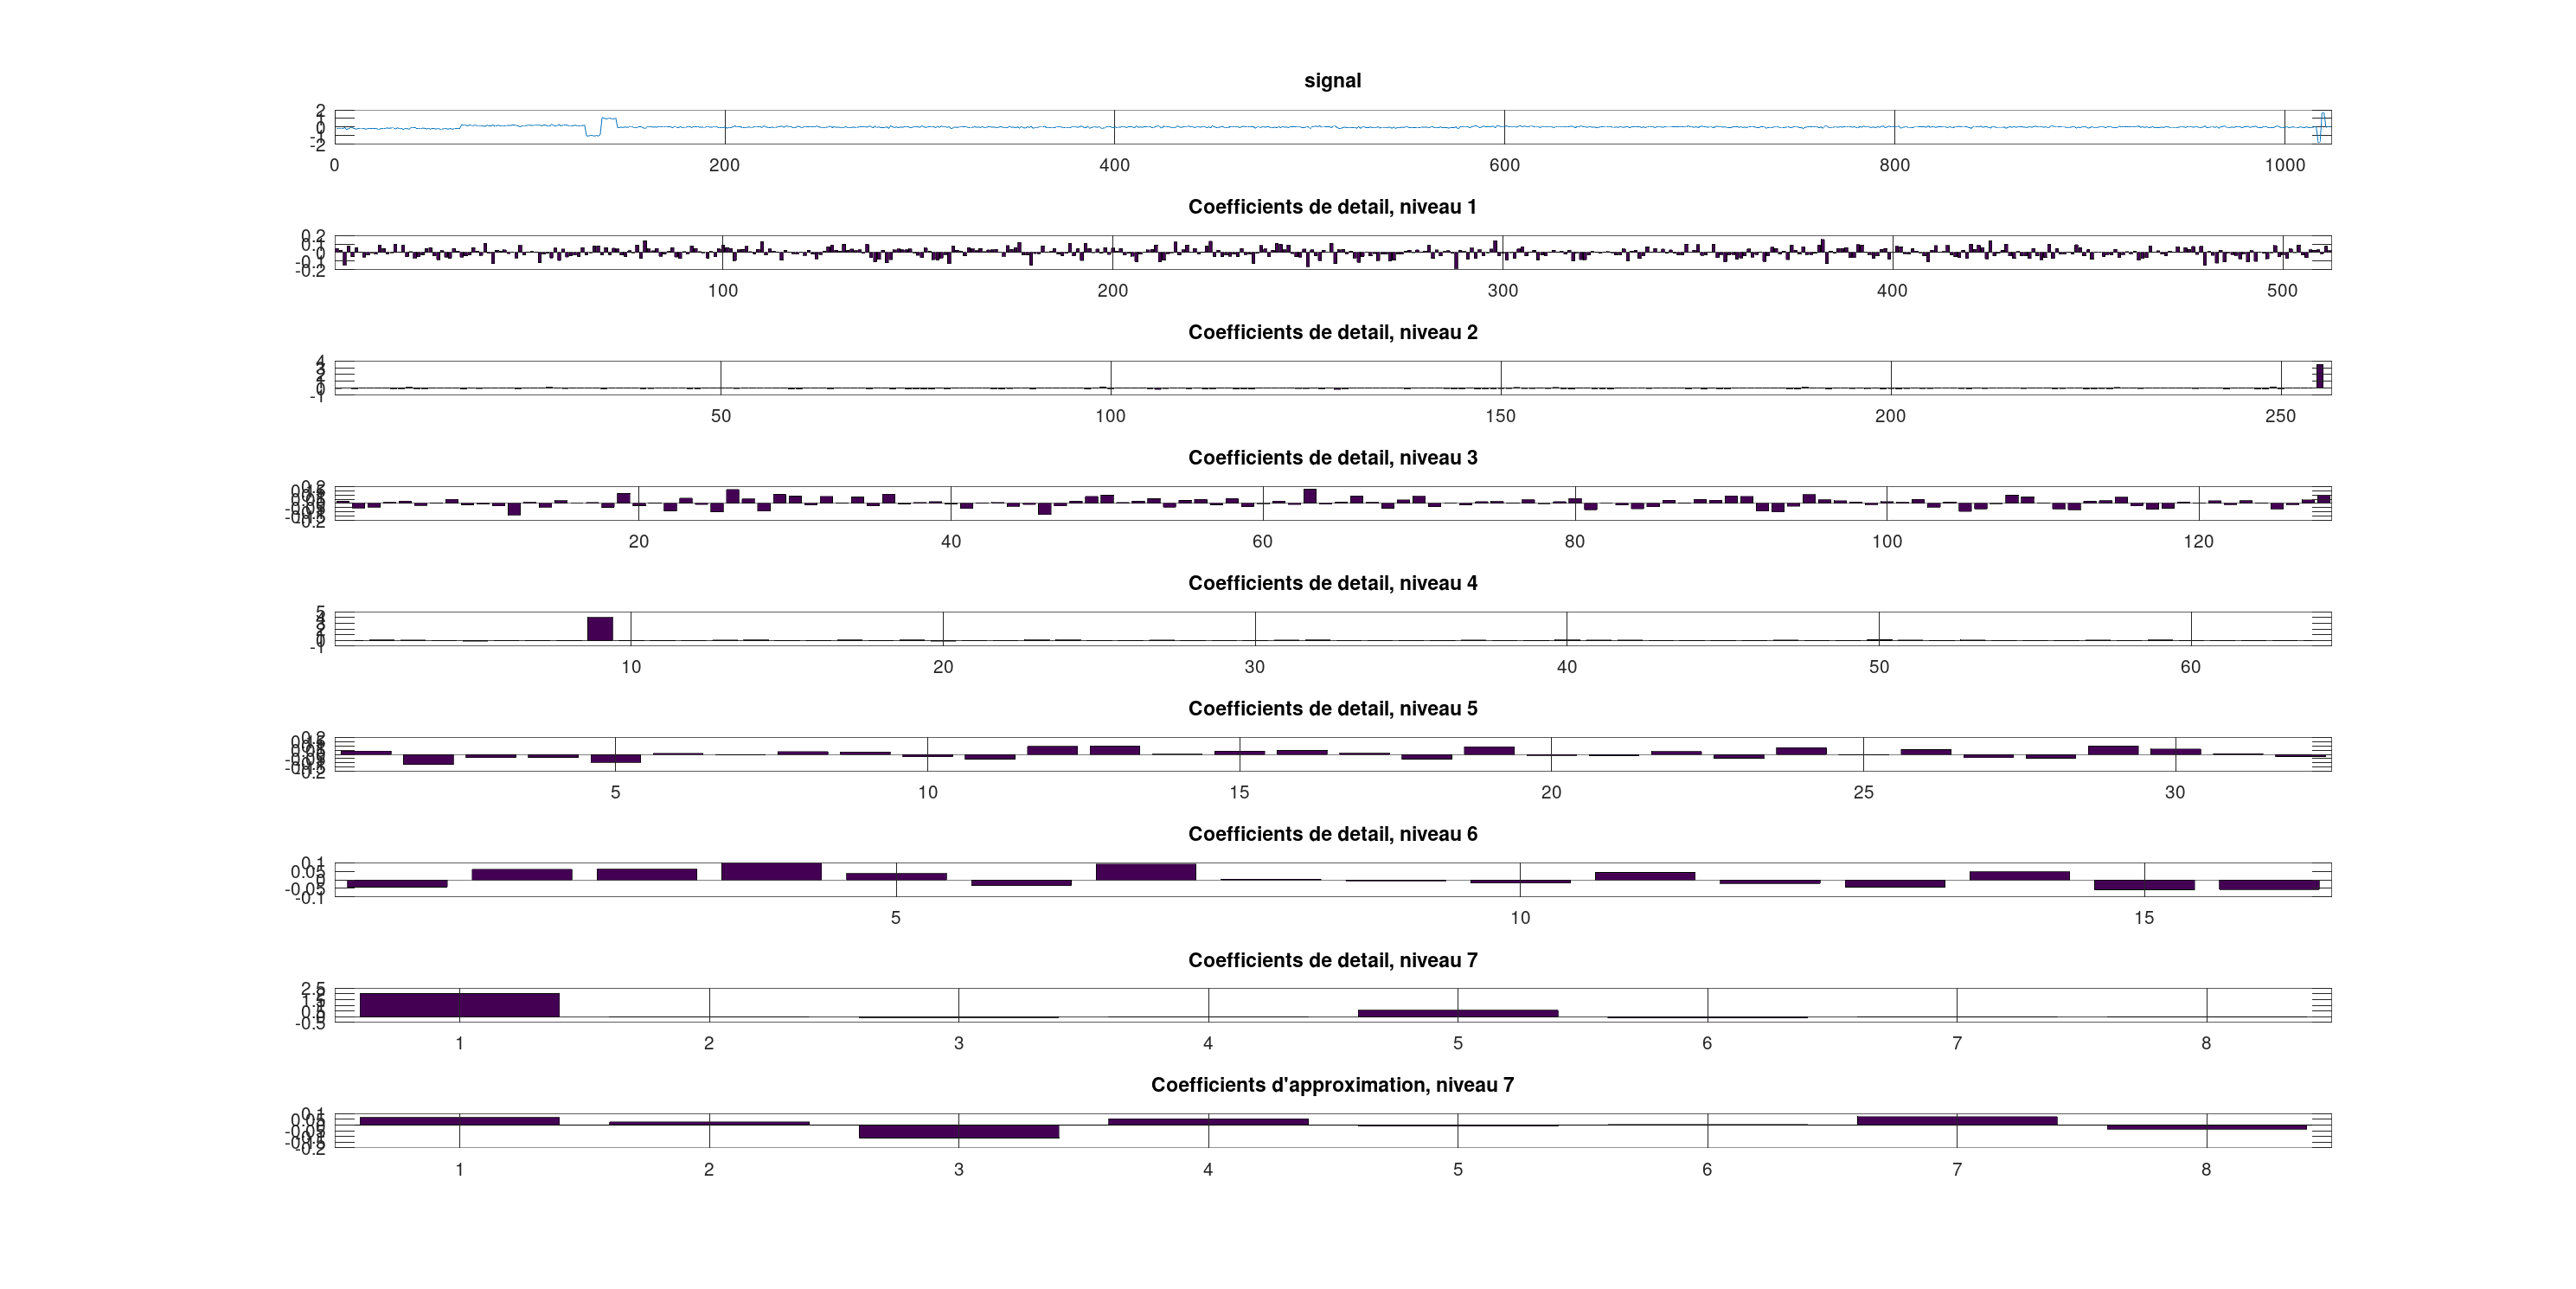
\includegraphics[width=\textwidth]{ex2_2}
                    \centering
                \end{figure}

                On observe ainsi que l'ajout de bruit au signal résulte
                également en un ajout de bruit à sa DWT. Toutefois on
                remarque que les nouveaux coefficients non nuls liés au
                bruit sont d'amplitude faible devant celle des coefficients
                de la DWT du signal sans bruit.Un filtrage des coefficients
                à l'aide d'un seuil devrait permettre un débruitage du signal.
            }

        \item{Mettons maintenant en œuvre le processus de débruitage décrit.
                Représentons alors l'erreur de construction commise en fonction
                de la valeur du seuil $\alpha$ et celle correspondant au seuil
                $\alpha^* = \sigma_b \sqrt{2 ln(N)}$ :

                \begin{figure}[H]
                    \caption{Erreur de reconstruction en fonction de alpha}
                    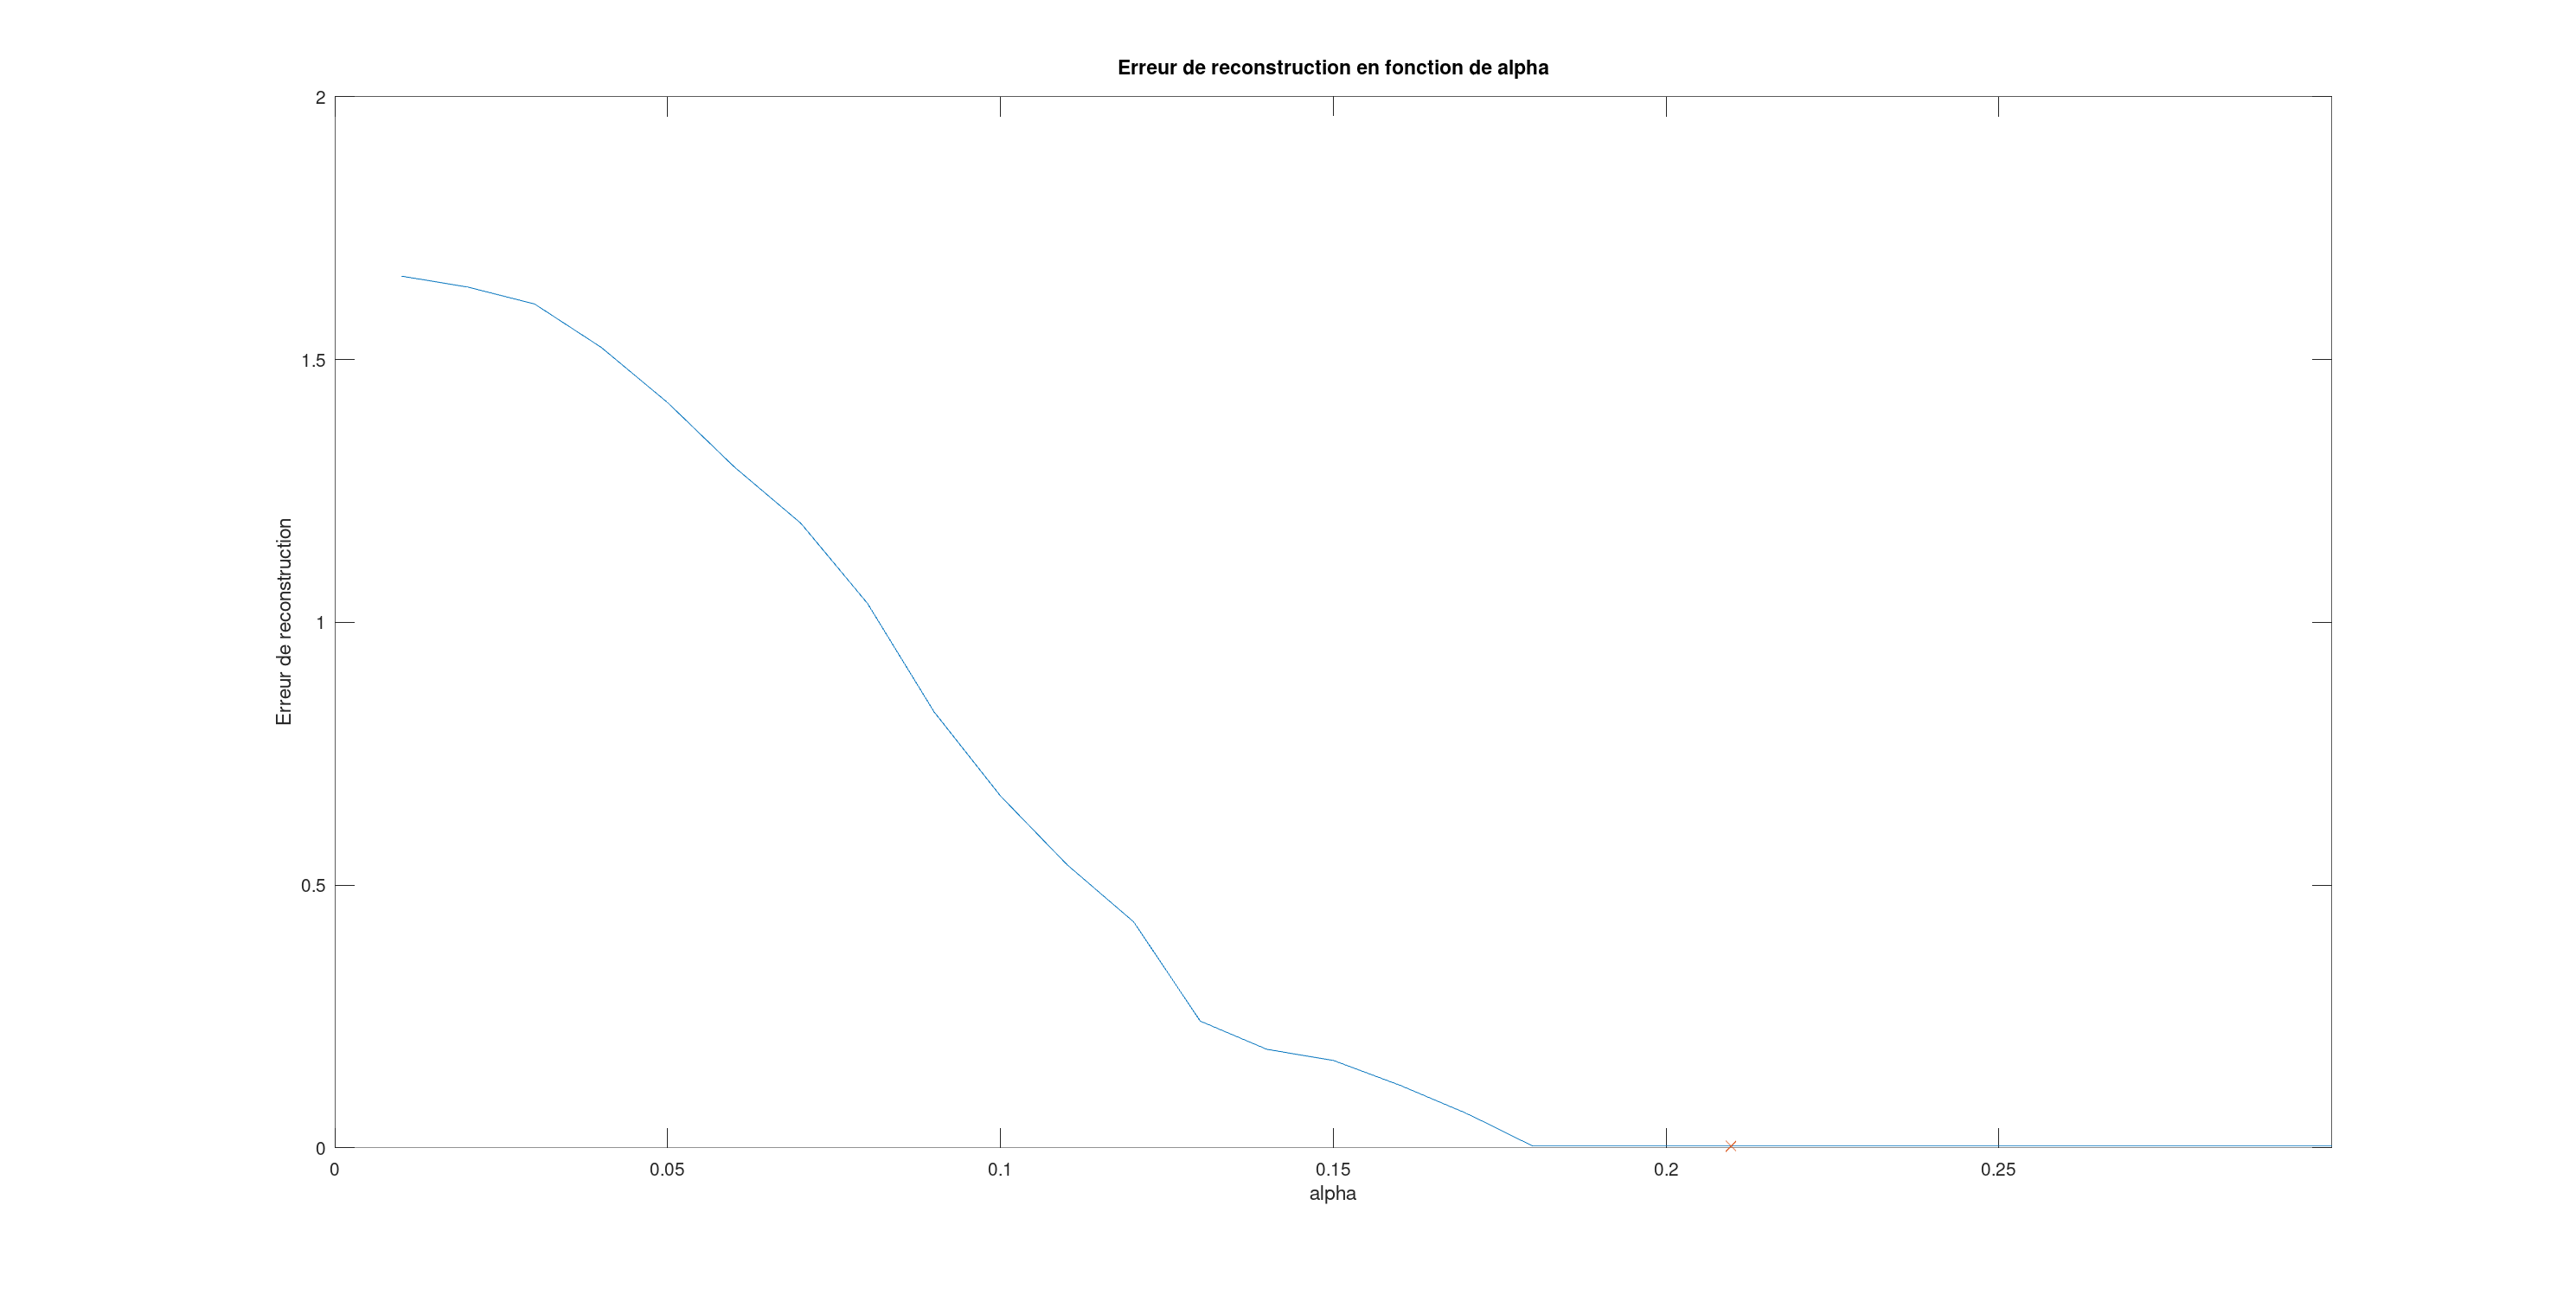
\includegraphics[width=\textwidth]{ex2_3}
                    \centering
                \end{figure}

                On obtient alors un seuil optimal correspondant à la valeur proposée.
            }

        \item{On génère les signaux "Blocks" et "Doppler" à l'aide de la
            fonction \texttt{makesig}.}

        \item{Représentons ces deux signaux ainsi que leur DWT :

                \begin{figure}[H]
                    \caption{Singal "Blocks"}
                    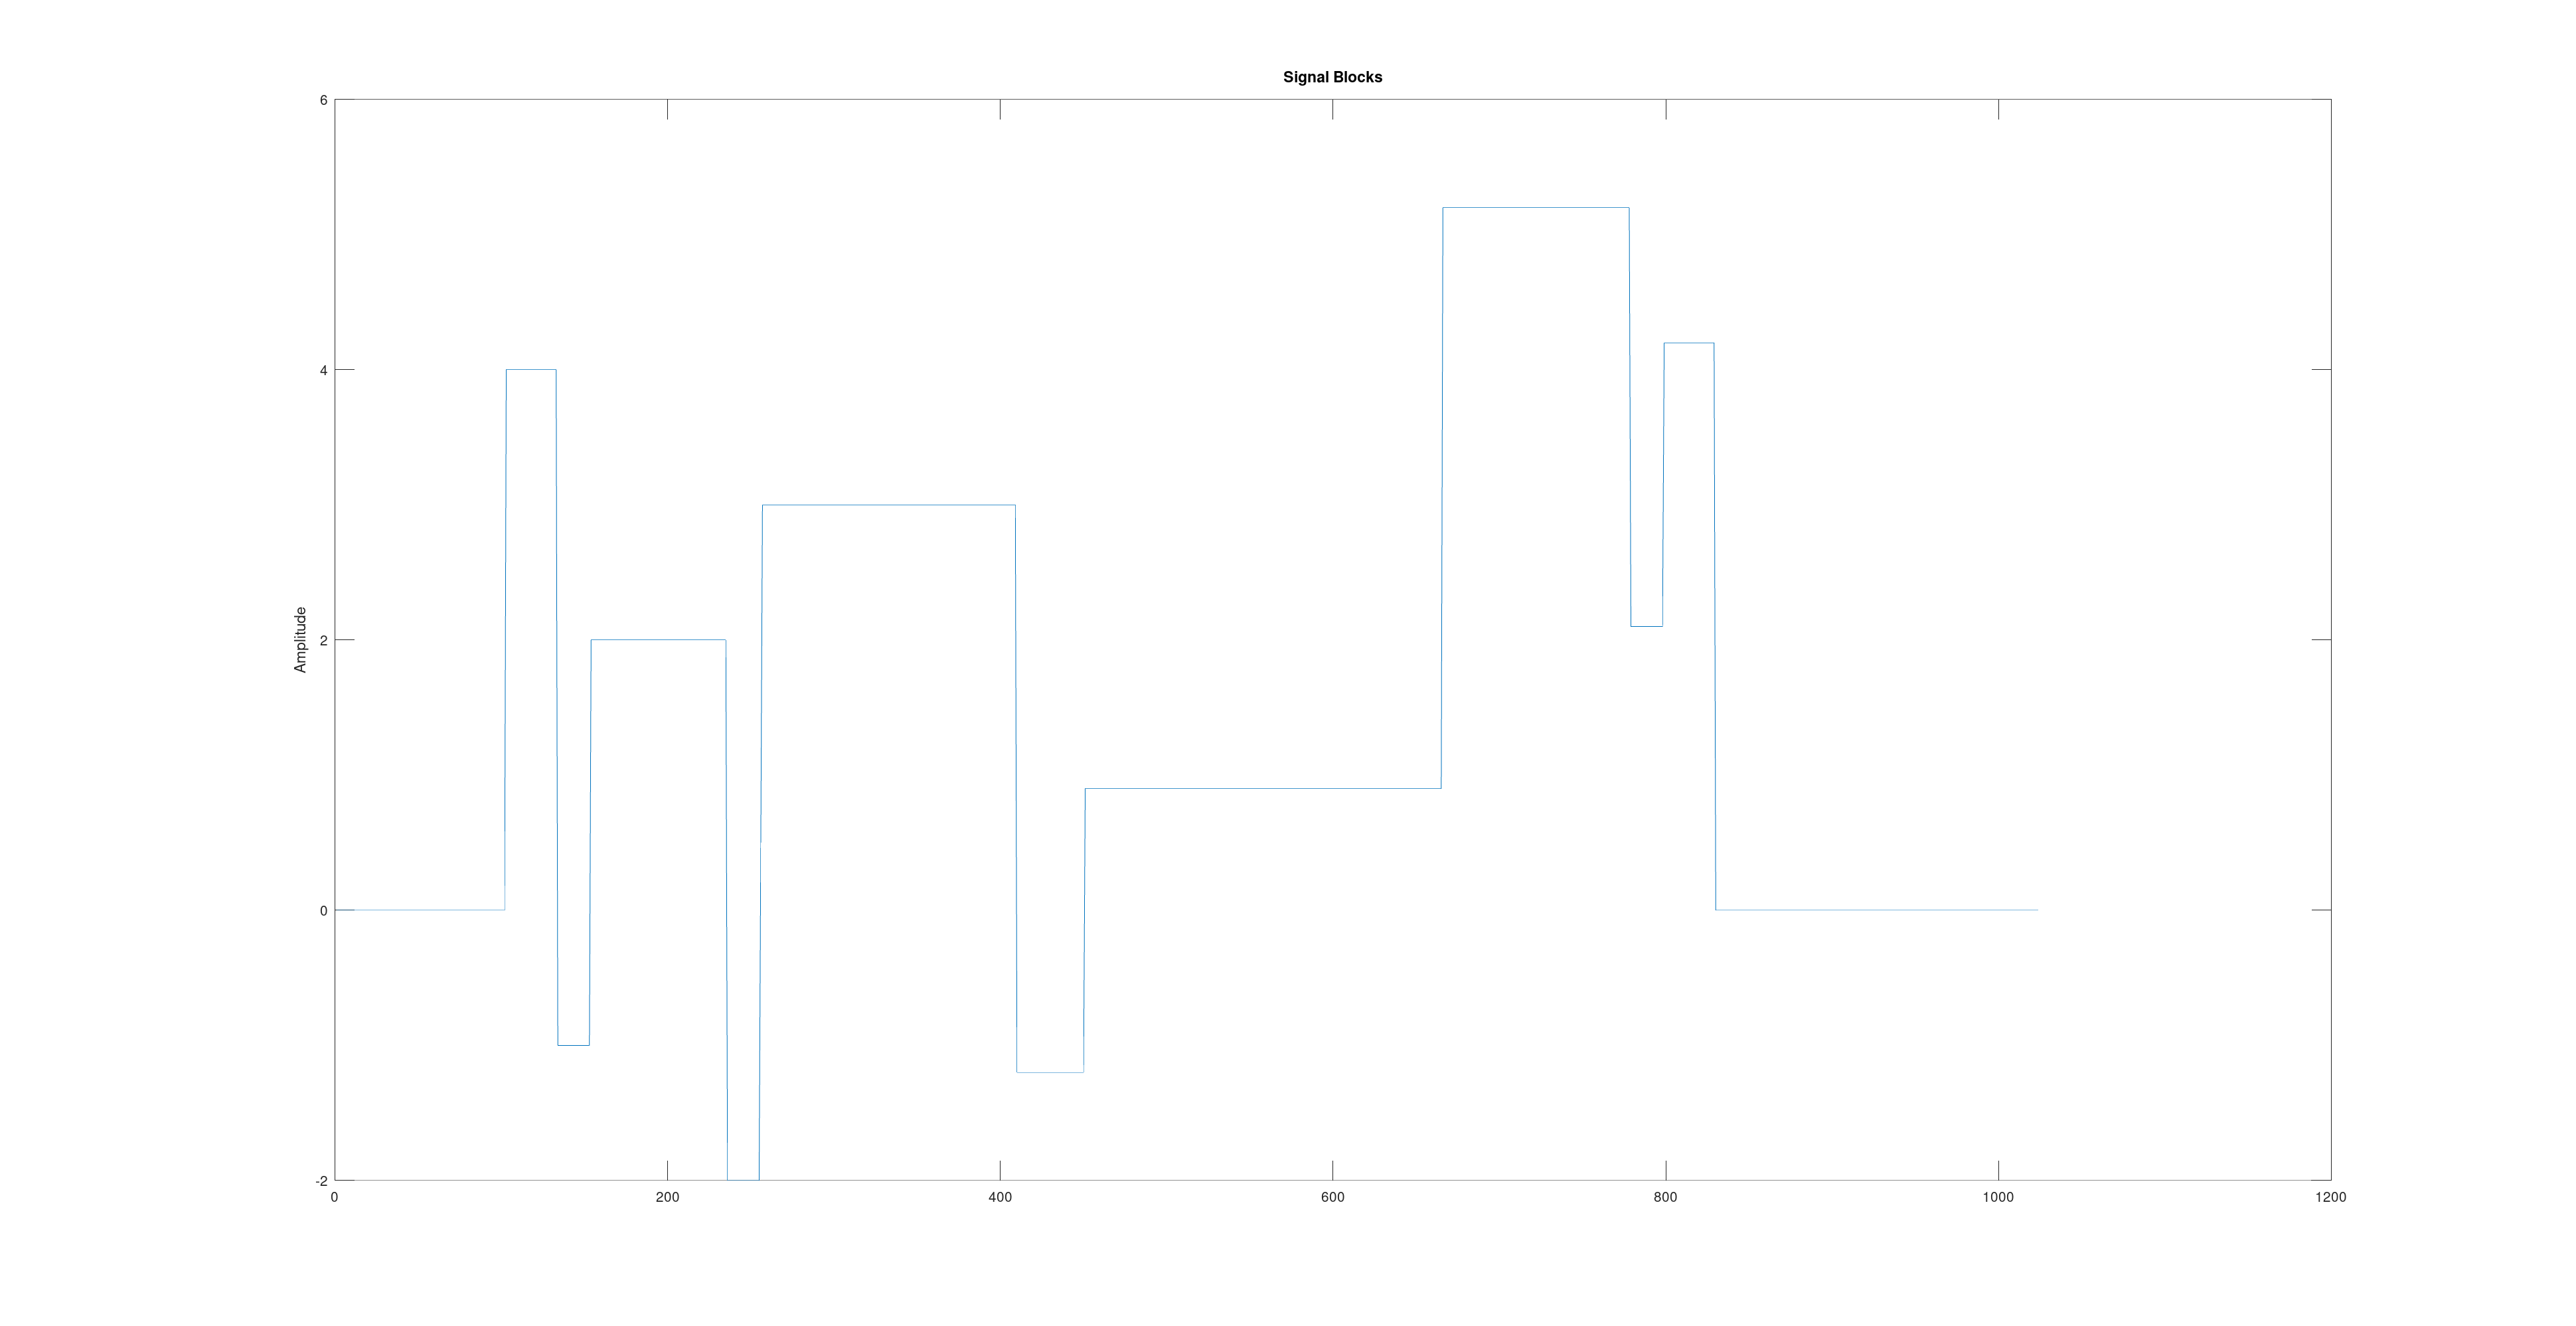
\includegraphics[width=\textwidth]{ex2_4_bis}
                    \centering
                \end{figure}

                \begin{figure}[H]
                    \caption{Singal "Blocks"}
                    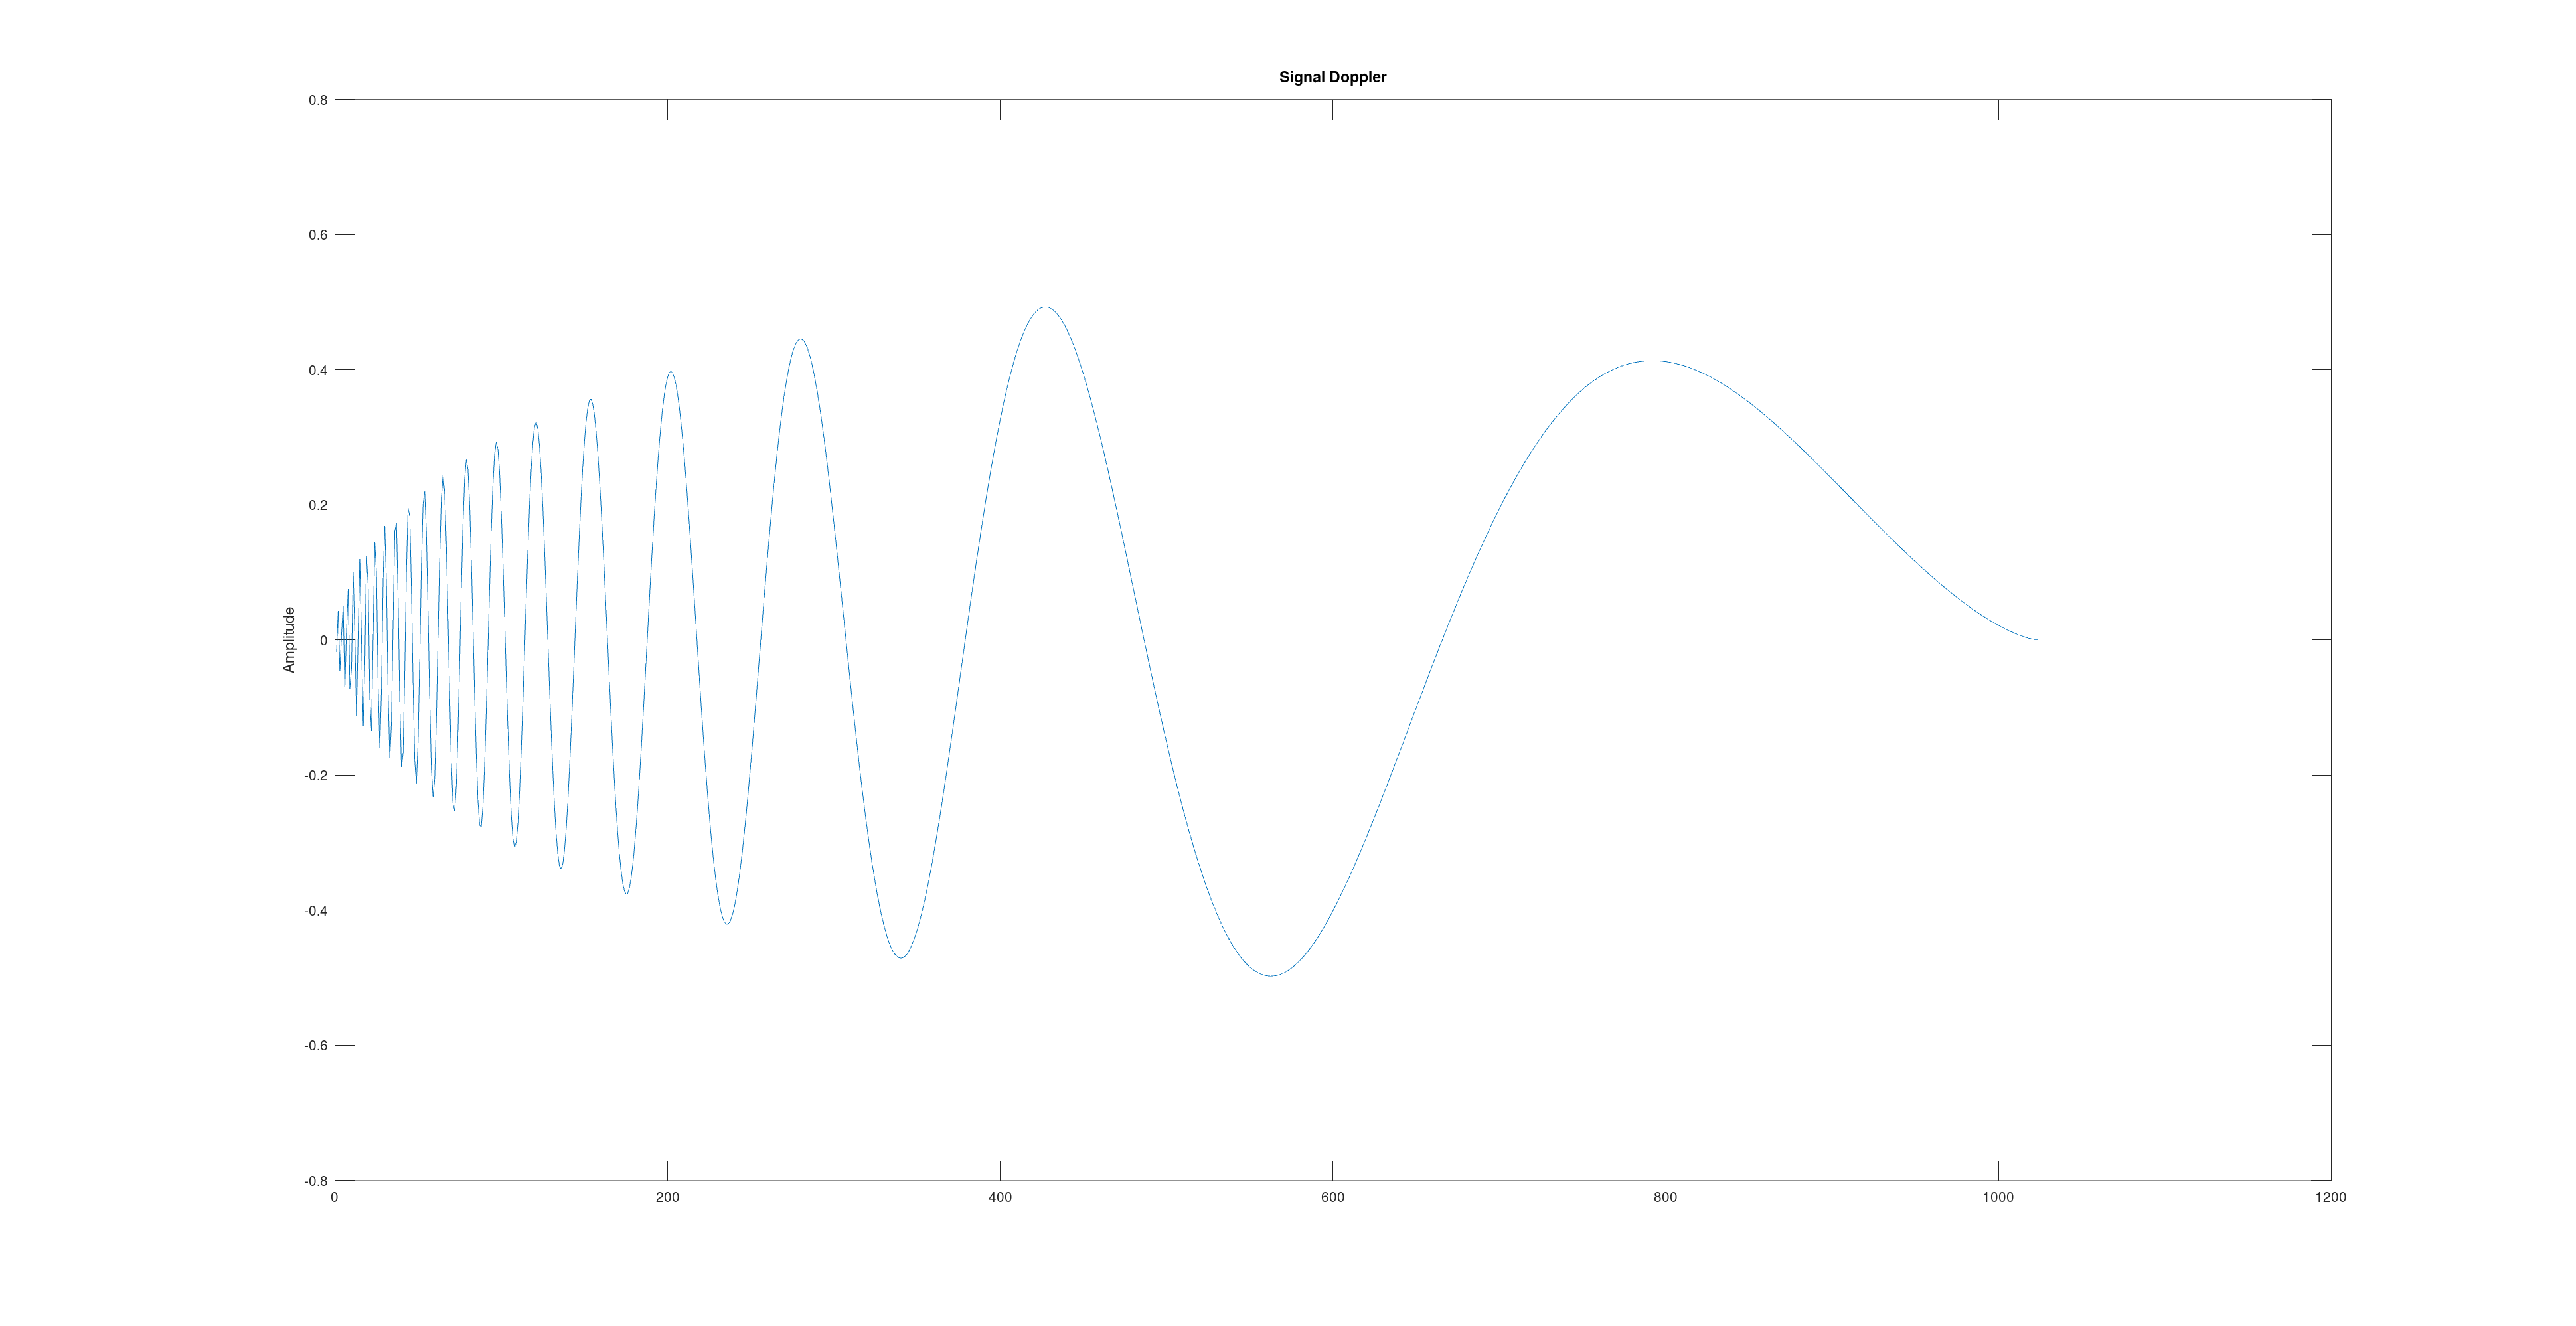
\includegraphics[width=\textwidth]{ex2_5_bis}
                    \centering
                \end{figure}

                \begin{figure}[H]
                    \caption{DWT signal "Blocks"}
                    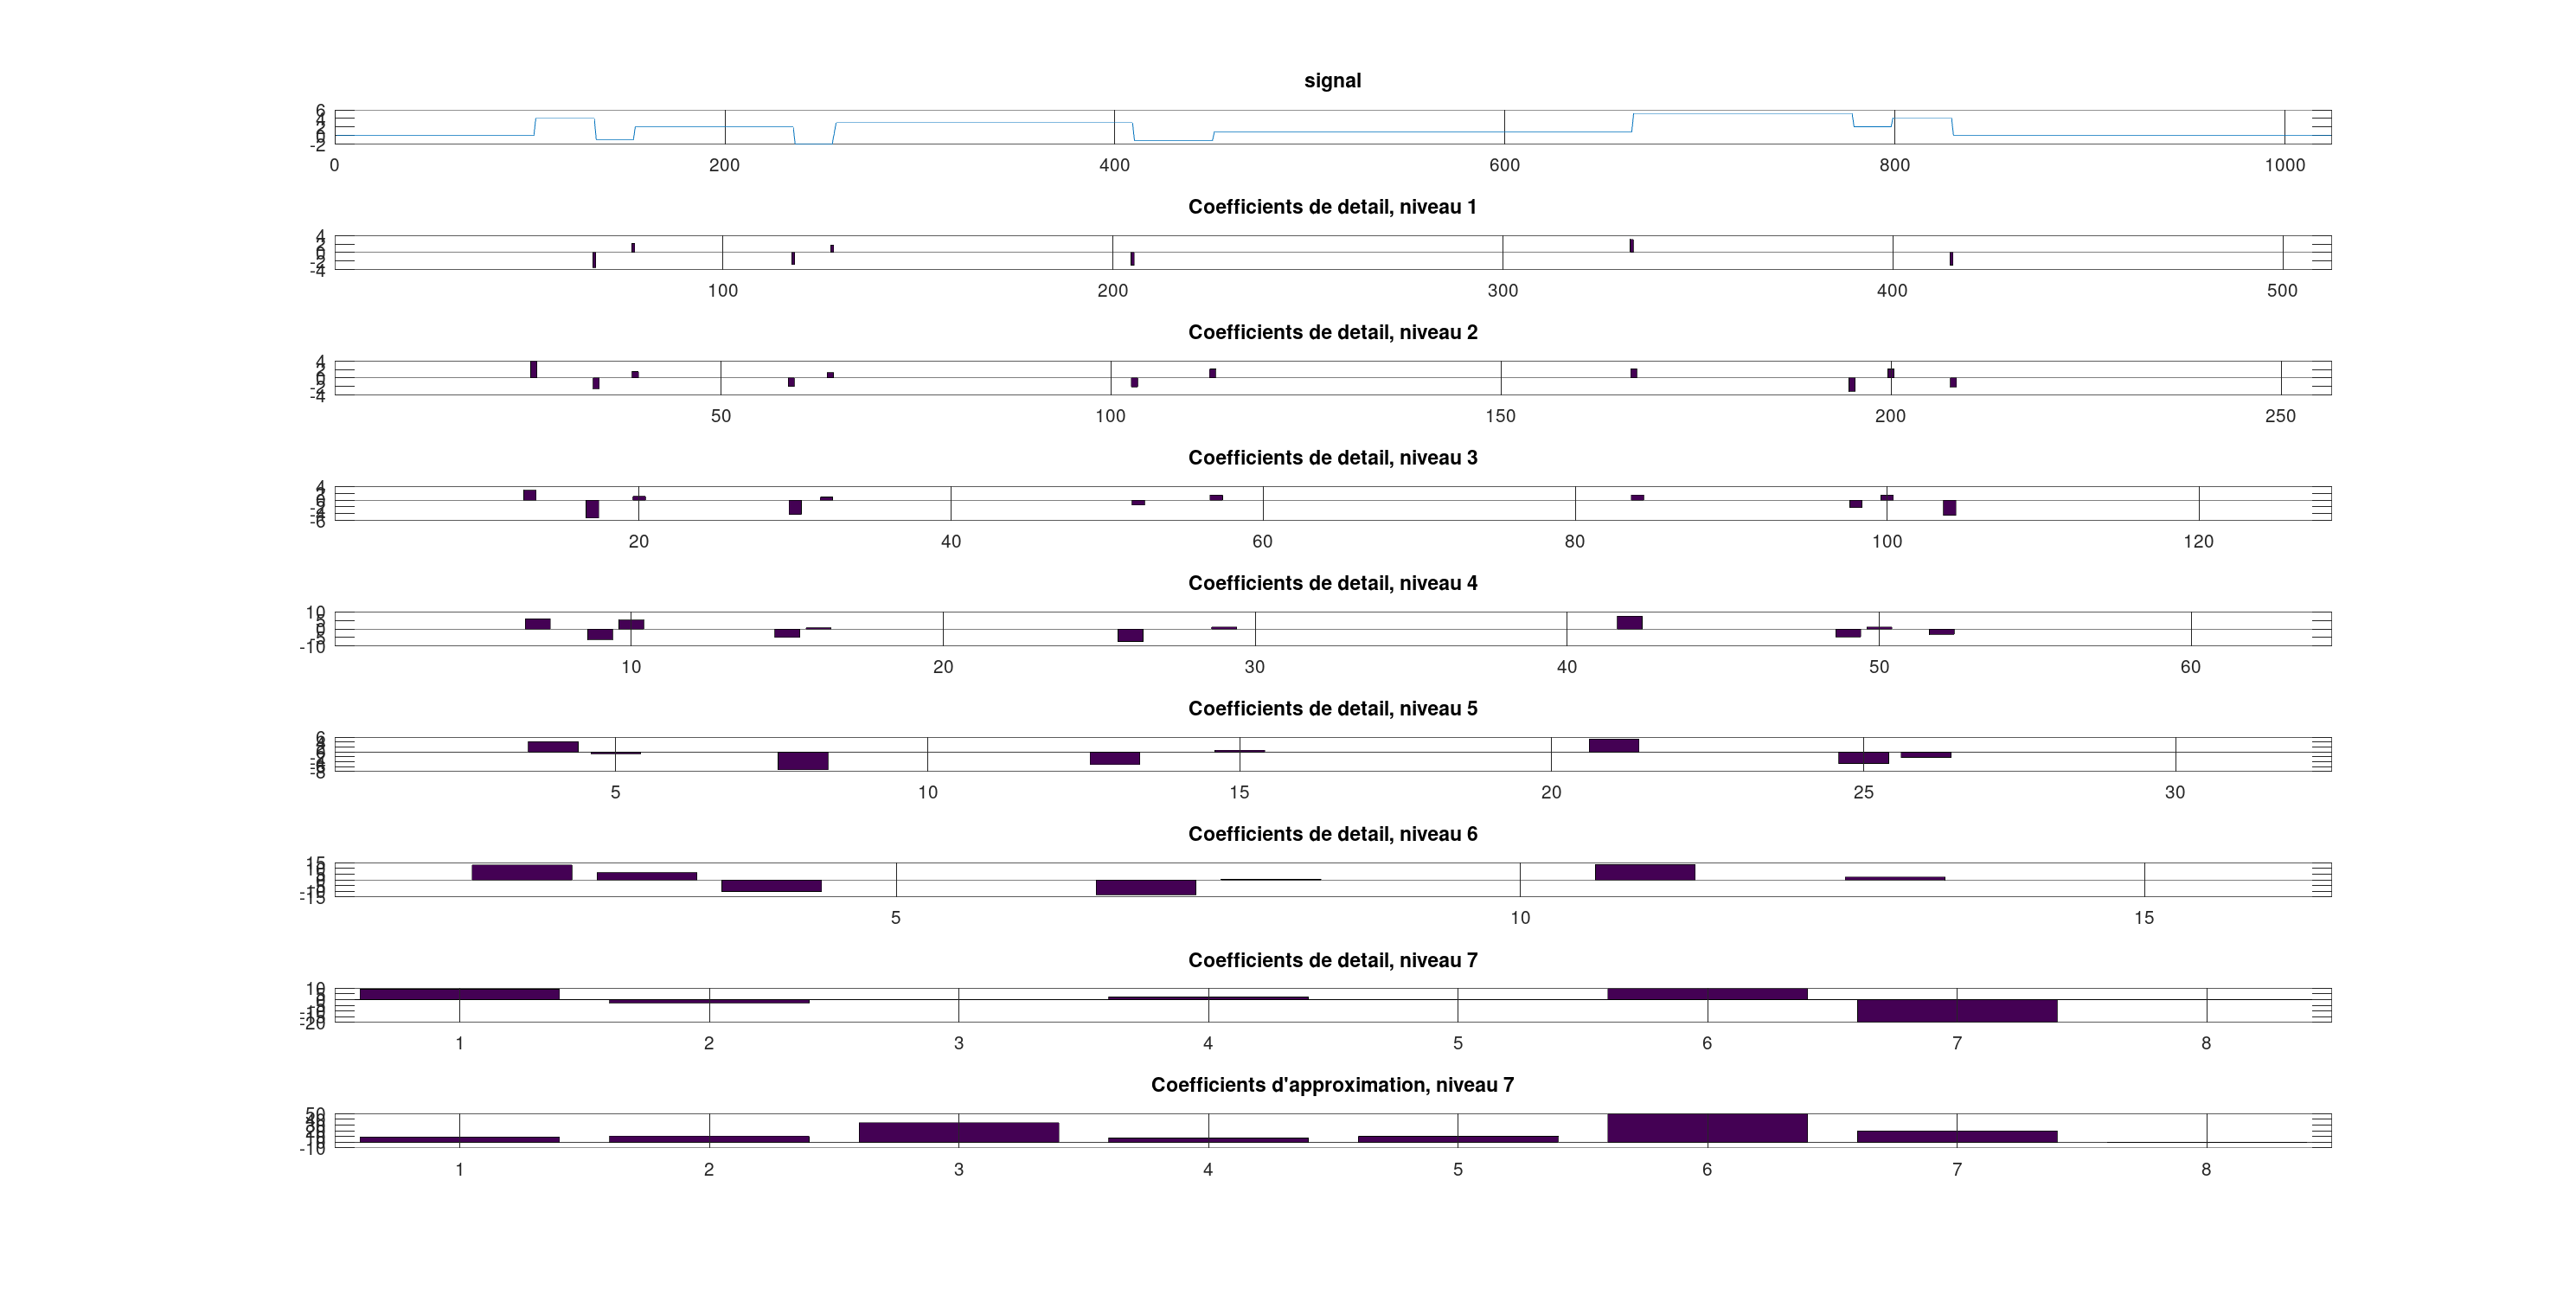
\includegraphics[width=\textwidth]{ex2_4}
                    \centering
                \end{figure}

                \begin{figure}[H]
                    \caption{DWT signal "Doppler"}
                    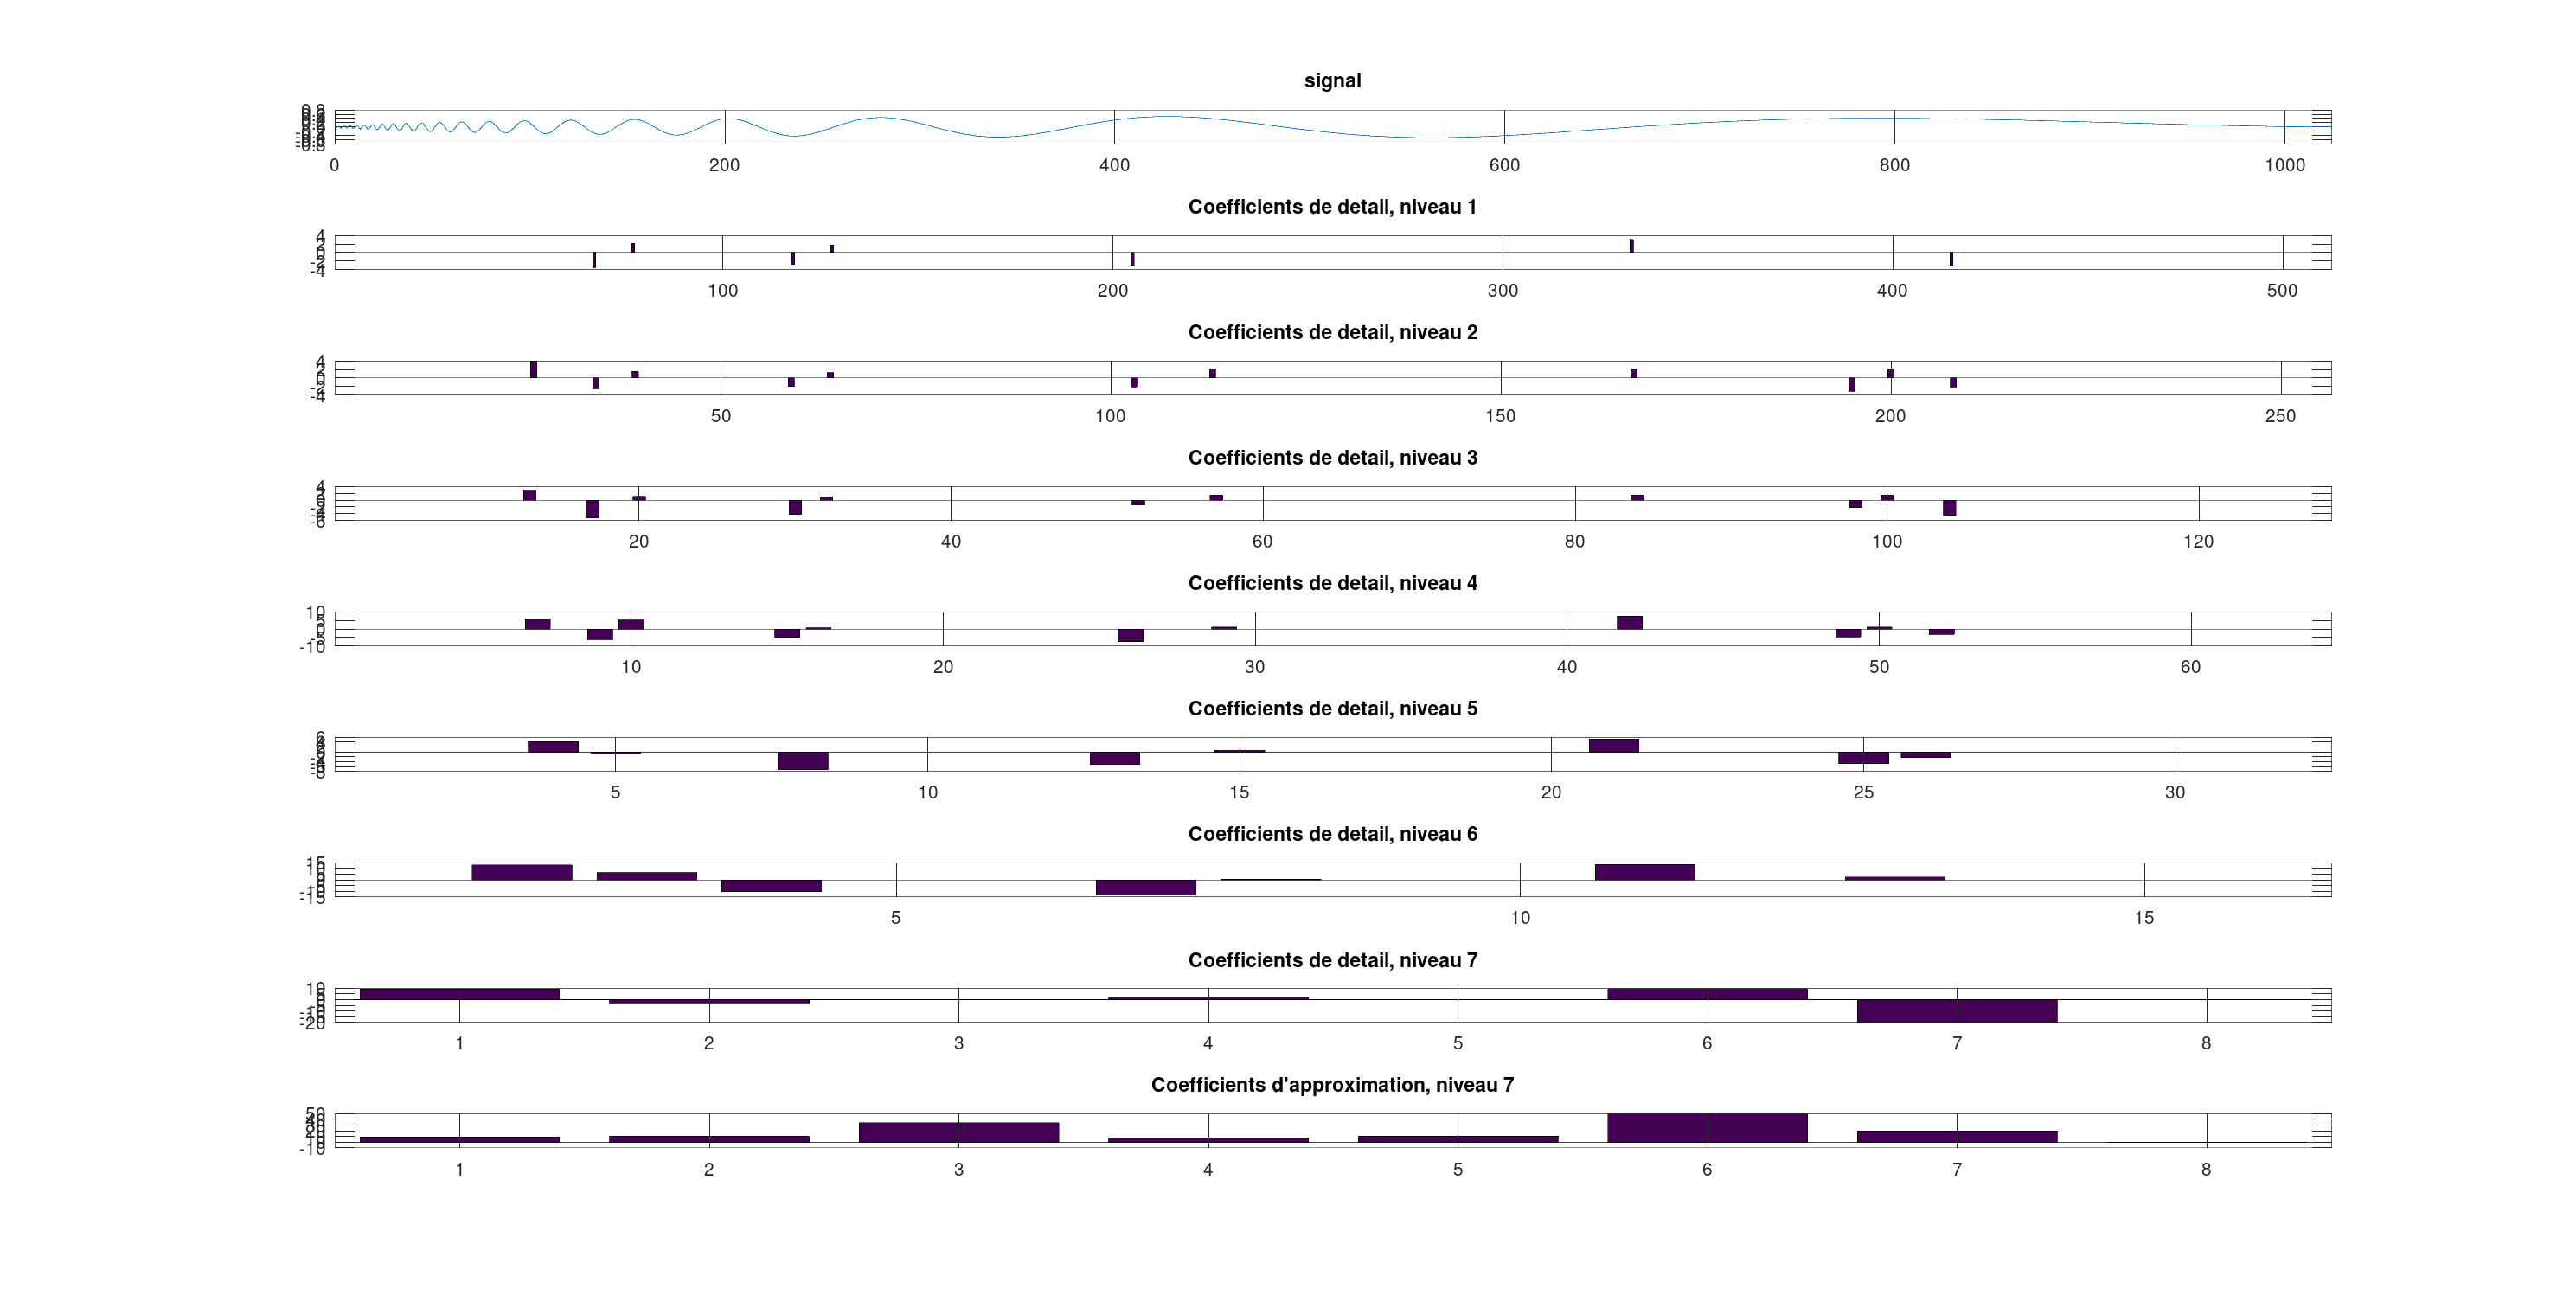
\includegraphics[width=\textwidth]{ex2_5}
                    \centering
                \end{figure}

                Ces signaux ont bien des allures cohérentes avec leurs noms. Les DWT disposent
                de plus de coefficients non nuls que pour le signal génèré précédemment

                Ajoutons du bruit avec un RSD de 20 dB et appliquons la
                procédure précédente. On obtient les tracés d'erreur de
                reconstruction en fonction du seuil suivants :

                \begin{figure}[H]
                    \caption{Erreur de reconstruction en fonction du seuil (Blocks)}
                    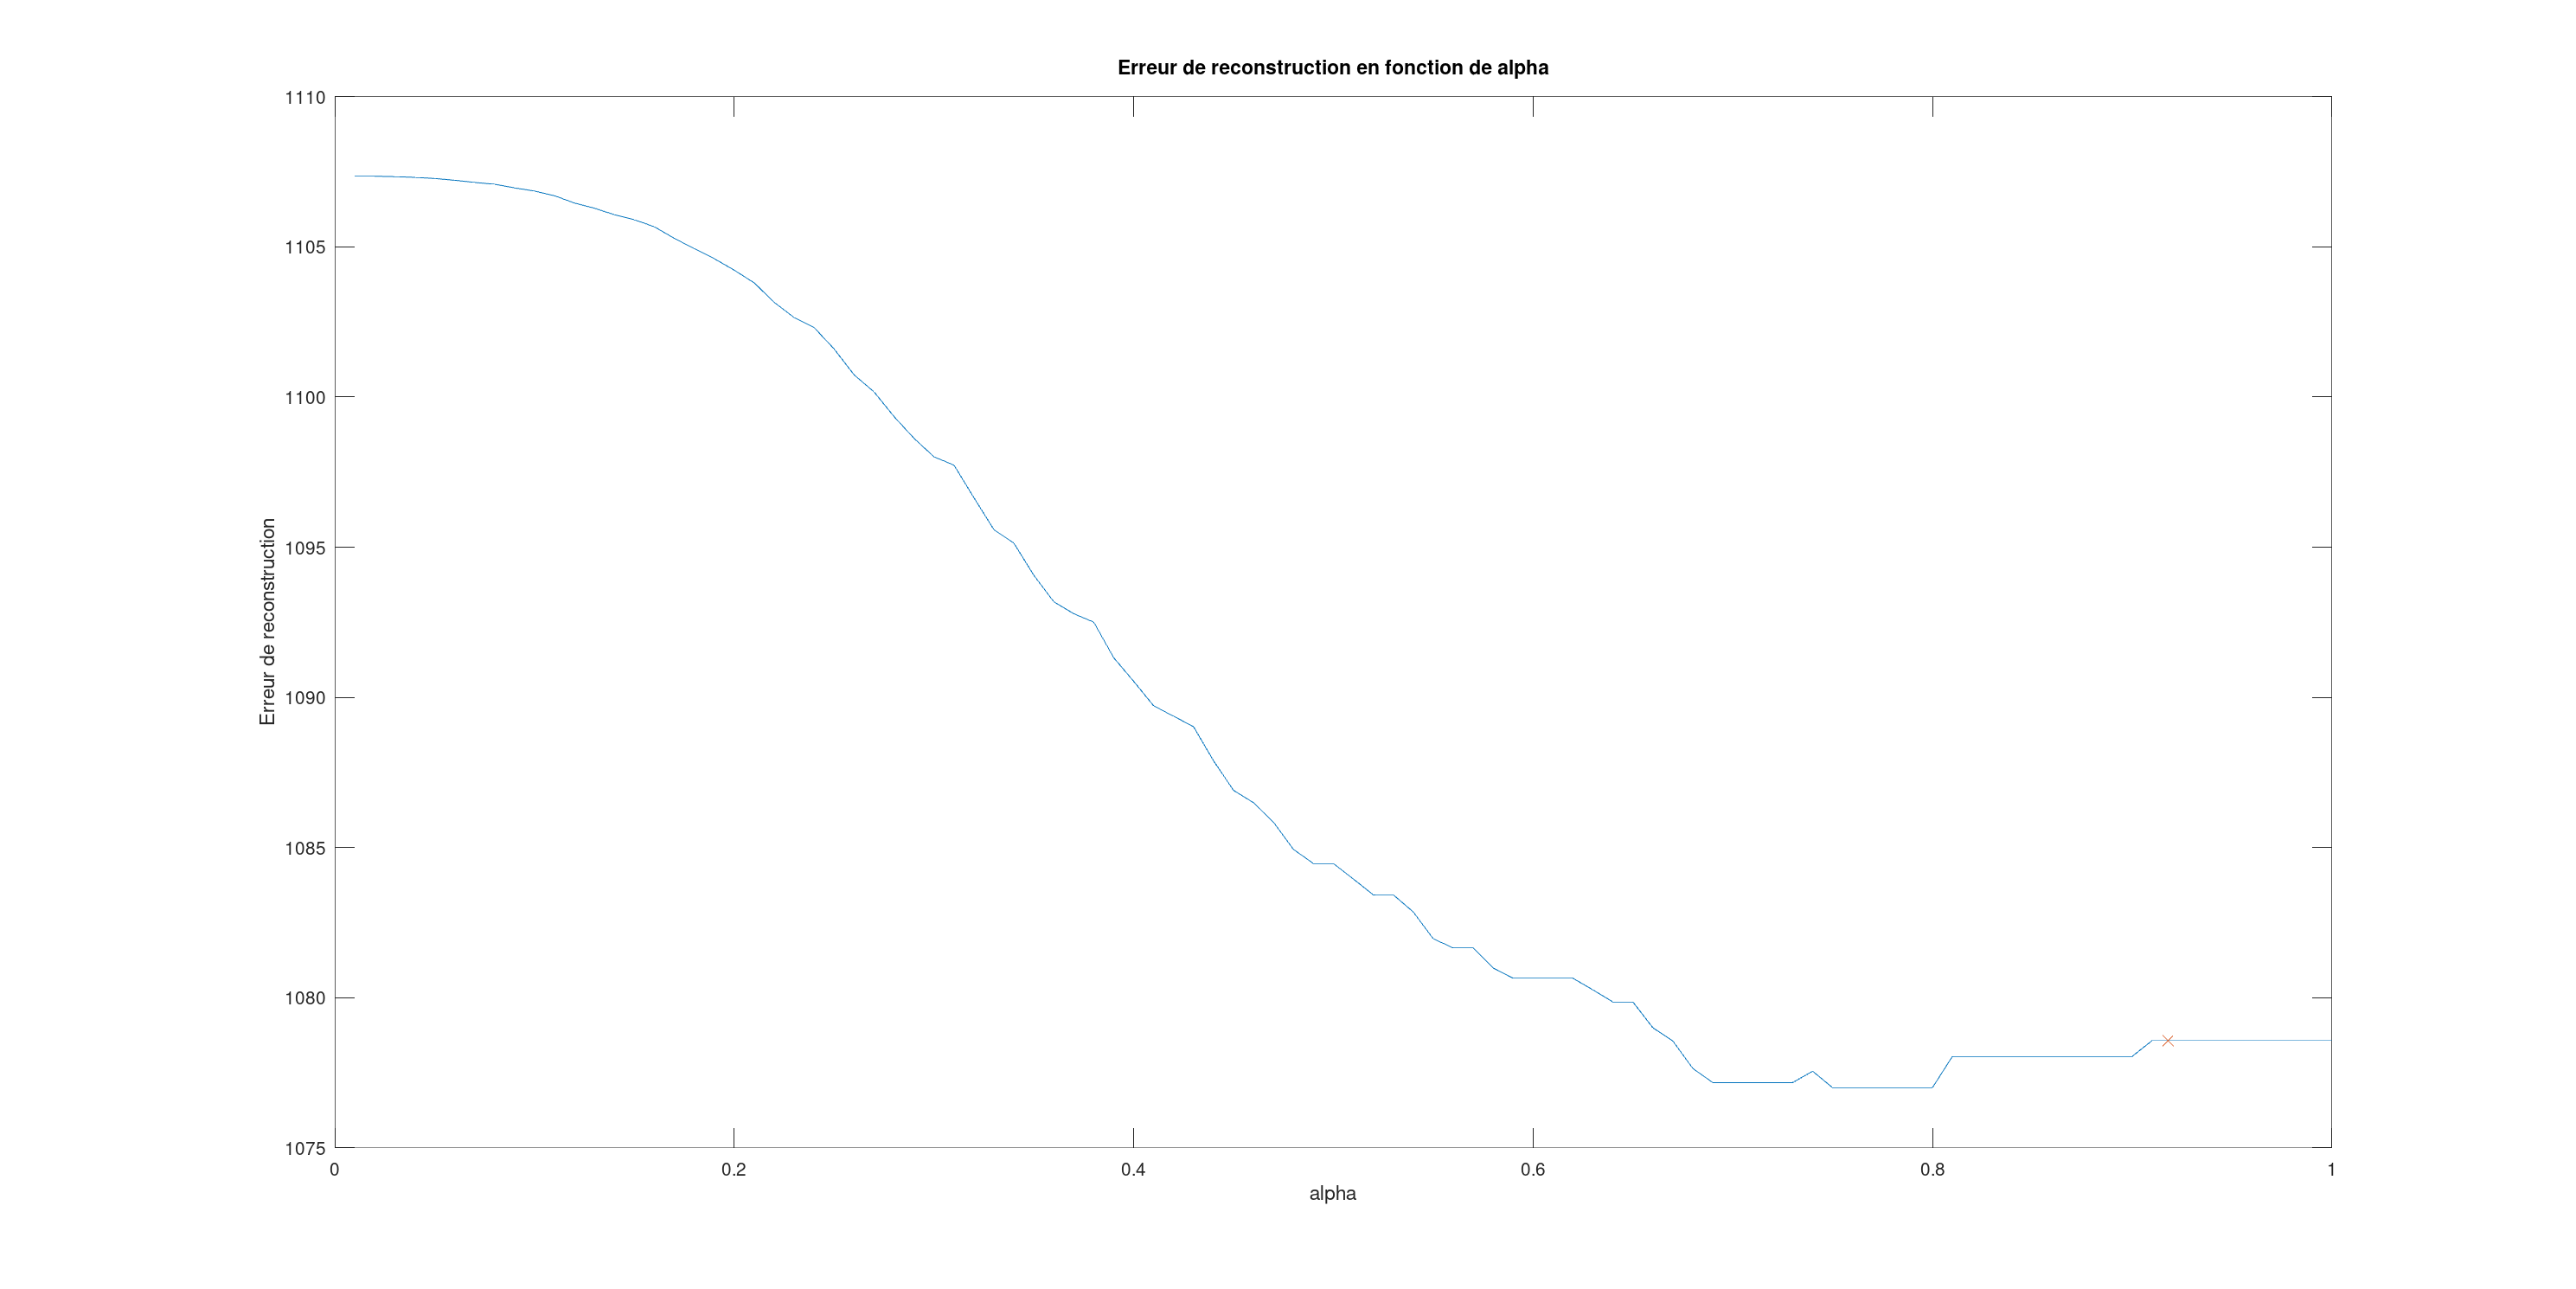
\includegraphics[width=\textwidth]{ex2_6}
                    \centering
                \end{figure}

                \begin{figure}[H]
                    \caption{Erreur de reconstruction en fonction du seuil (Dopler)}
                    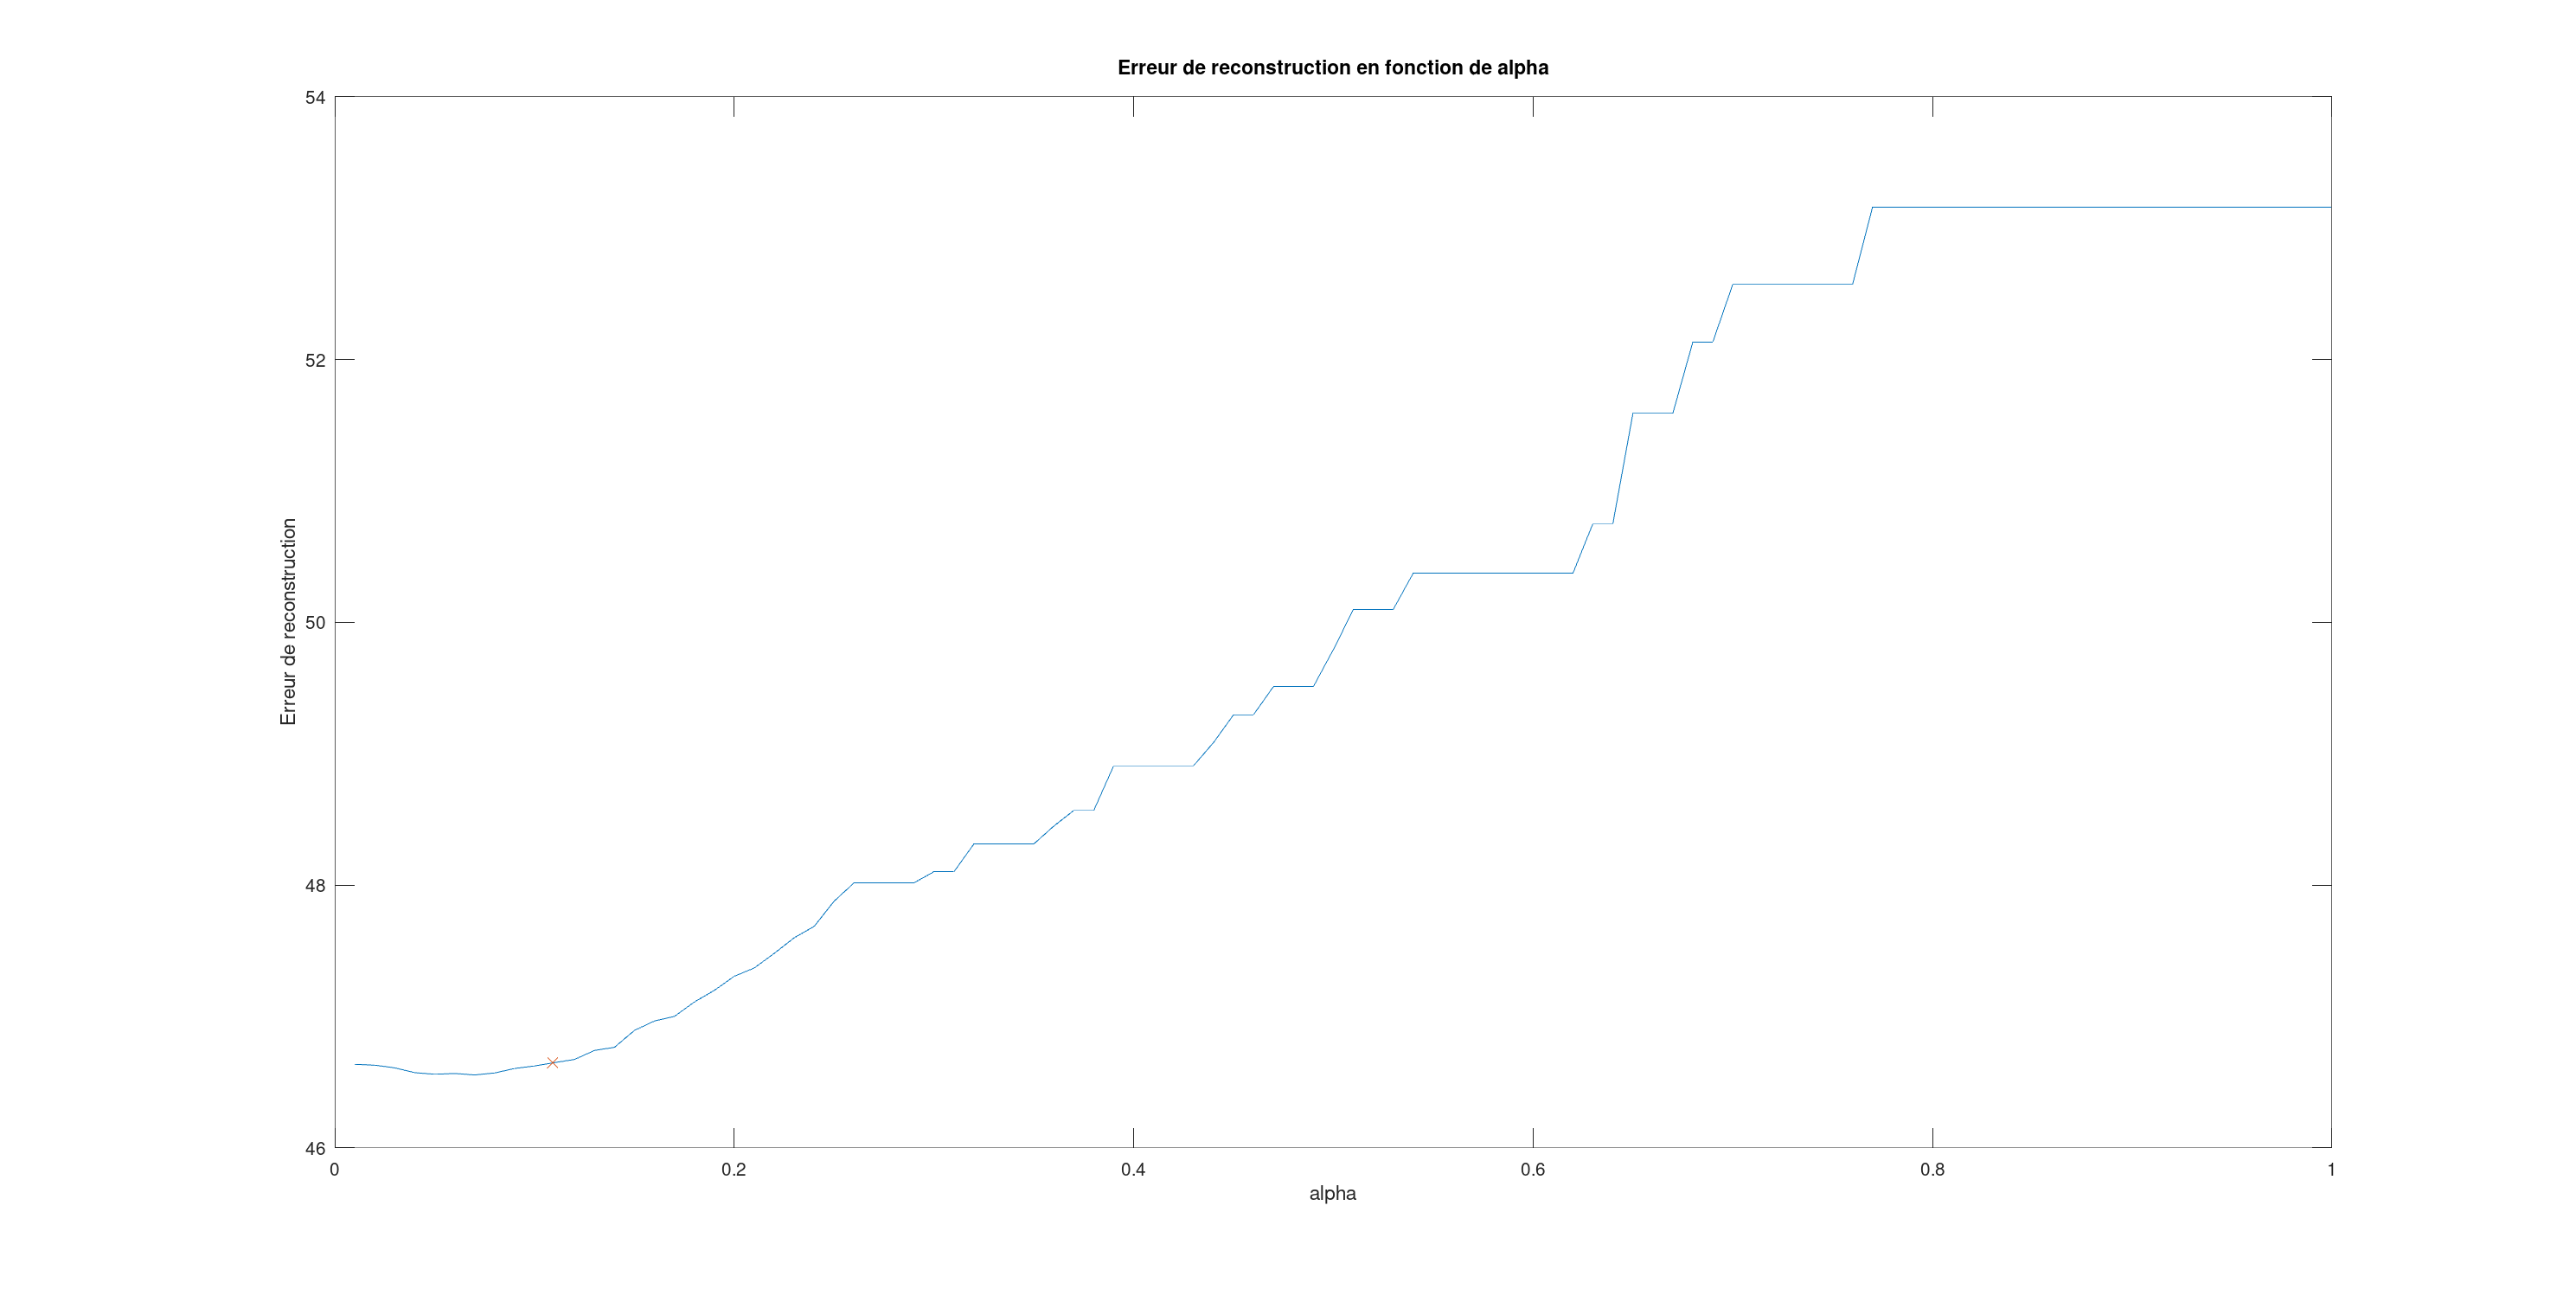
\includegraphics[width=\textwidth]{ex2_7}
                    \centering
                \end{figure}

                On obtient cette fois pour le signal "Blocks" une valeur de seuil optimale différente
                de celle proposée mais une valeur comparable dans le cas du signal "Doppler".
            }

        \item{En utilisant maintenant une ondelette de Daubechies d'ordre 4,
                on obtient les tracés suivants :

                \begin{figure}[H]
                    \caption{Erreur de reconstruction en fonction du seuil (Blocks)}
                    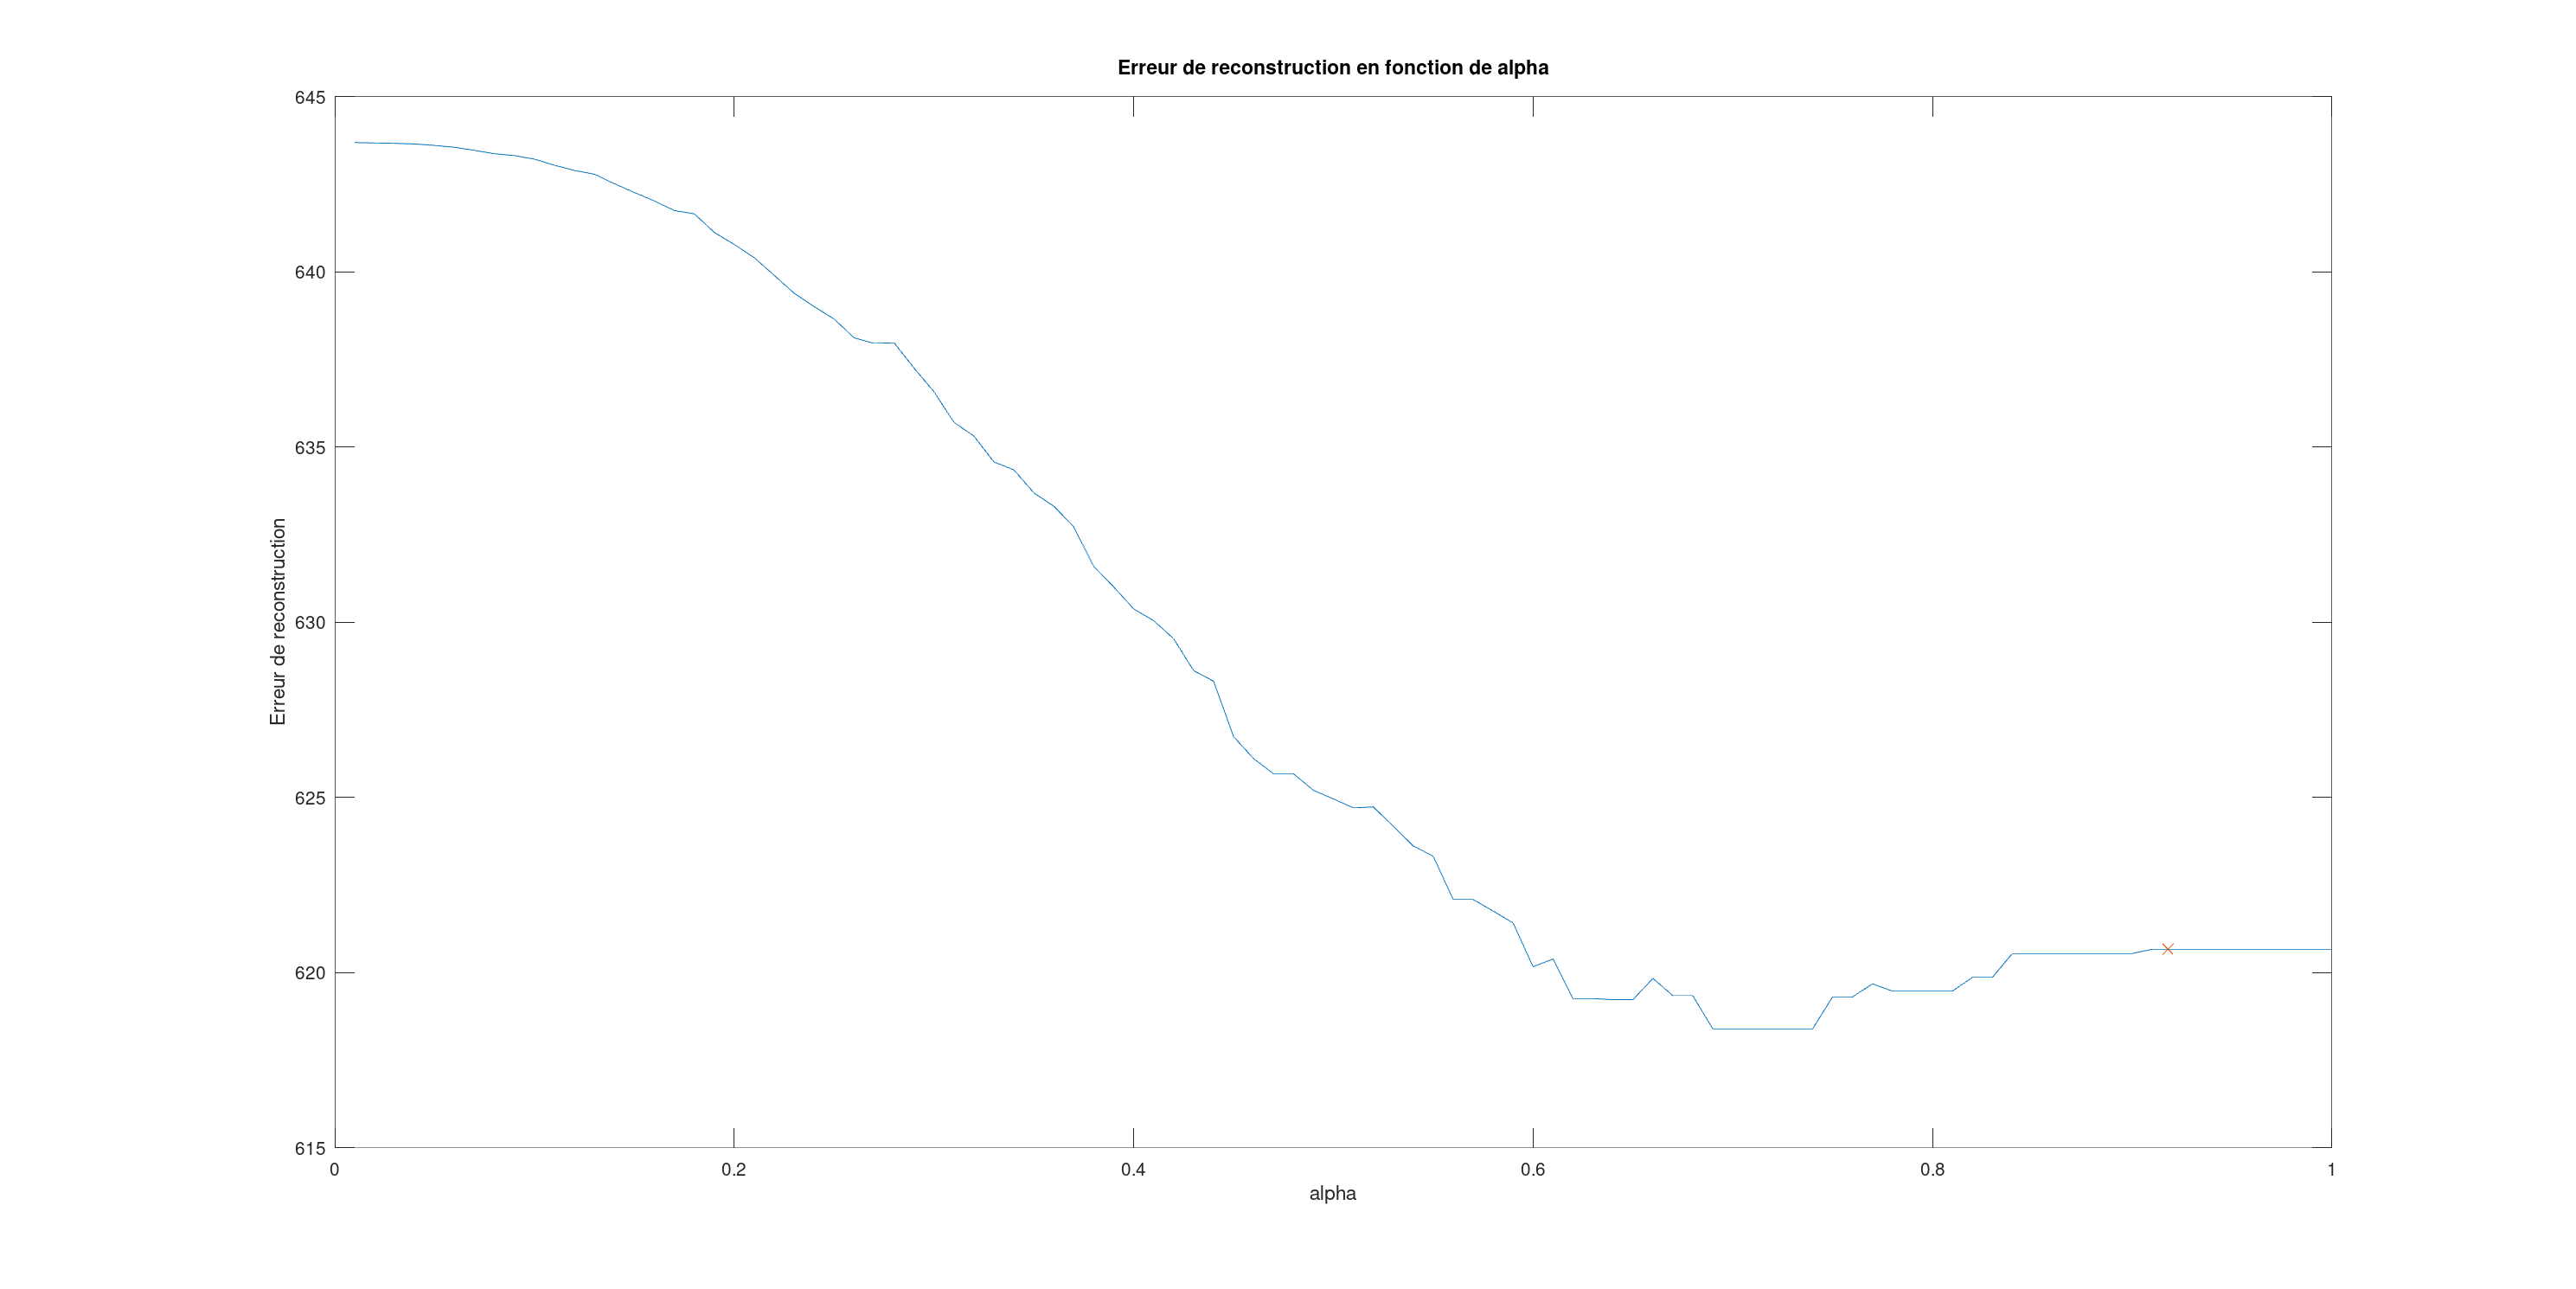
\includegraphics[width=\textwidth]{ex2_6bis}
                    \centering
                \end{figure}

                \begin{figure}[H]
                    \caption{Erreur de reconstruction en fonction du seuil (Dopler)}
                    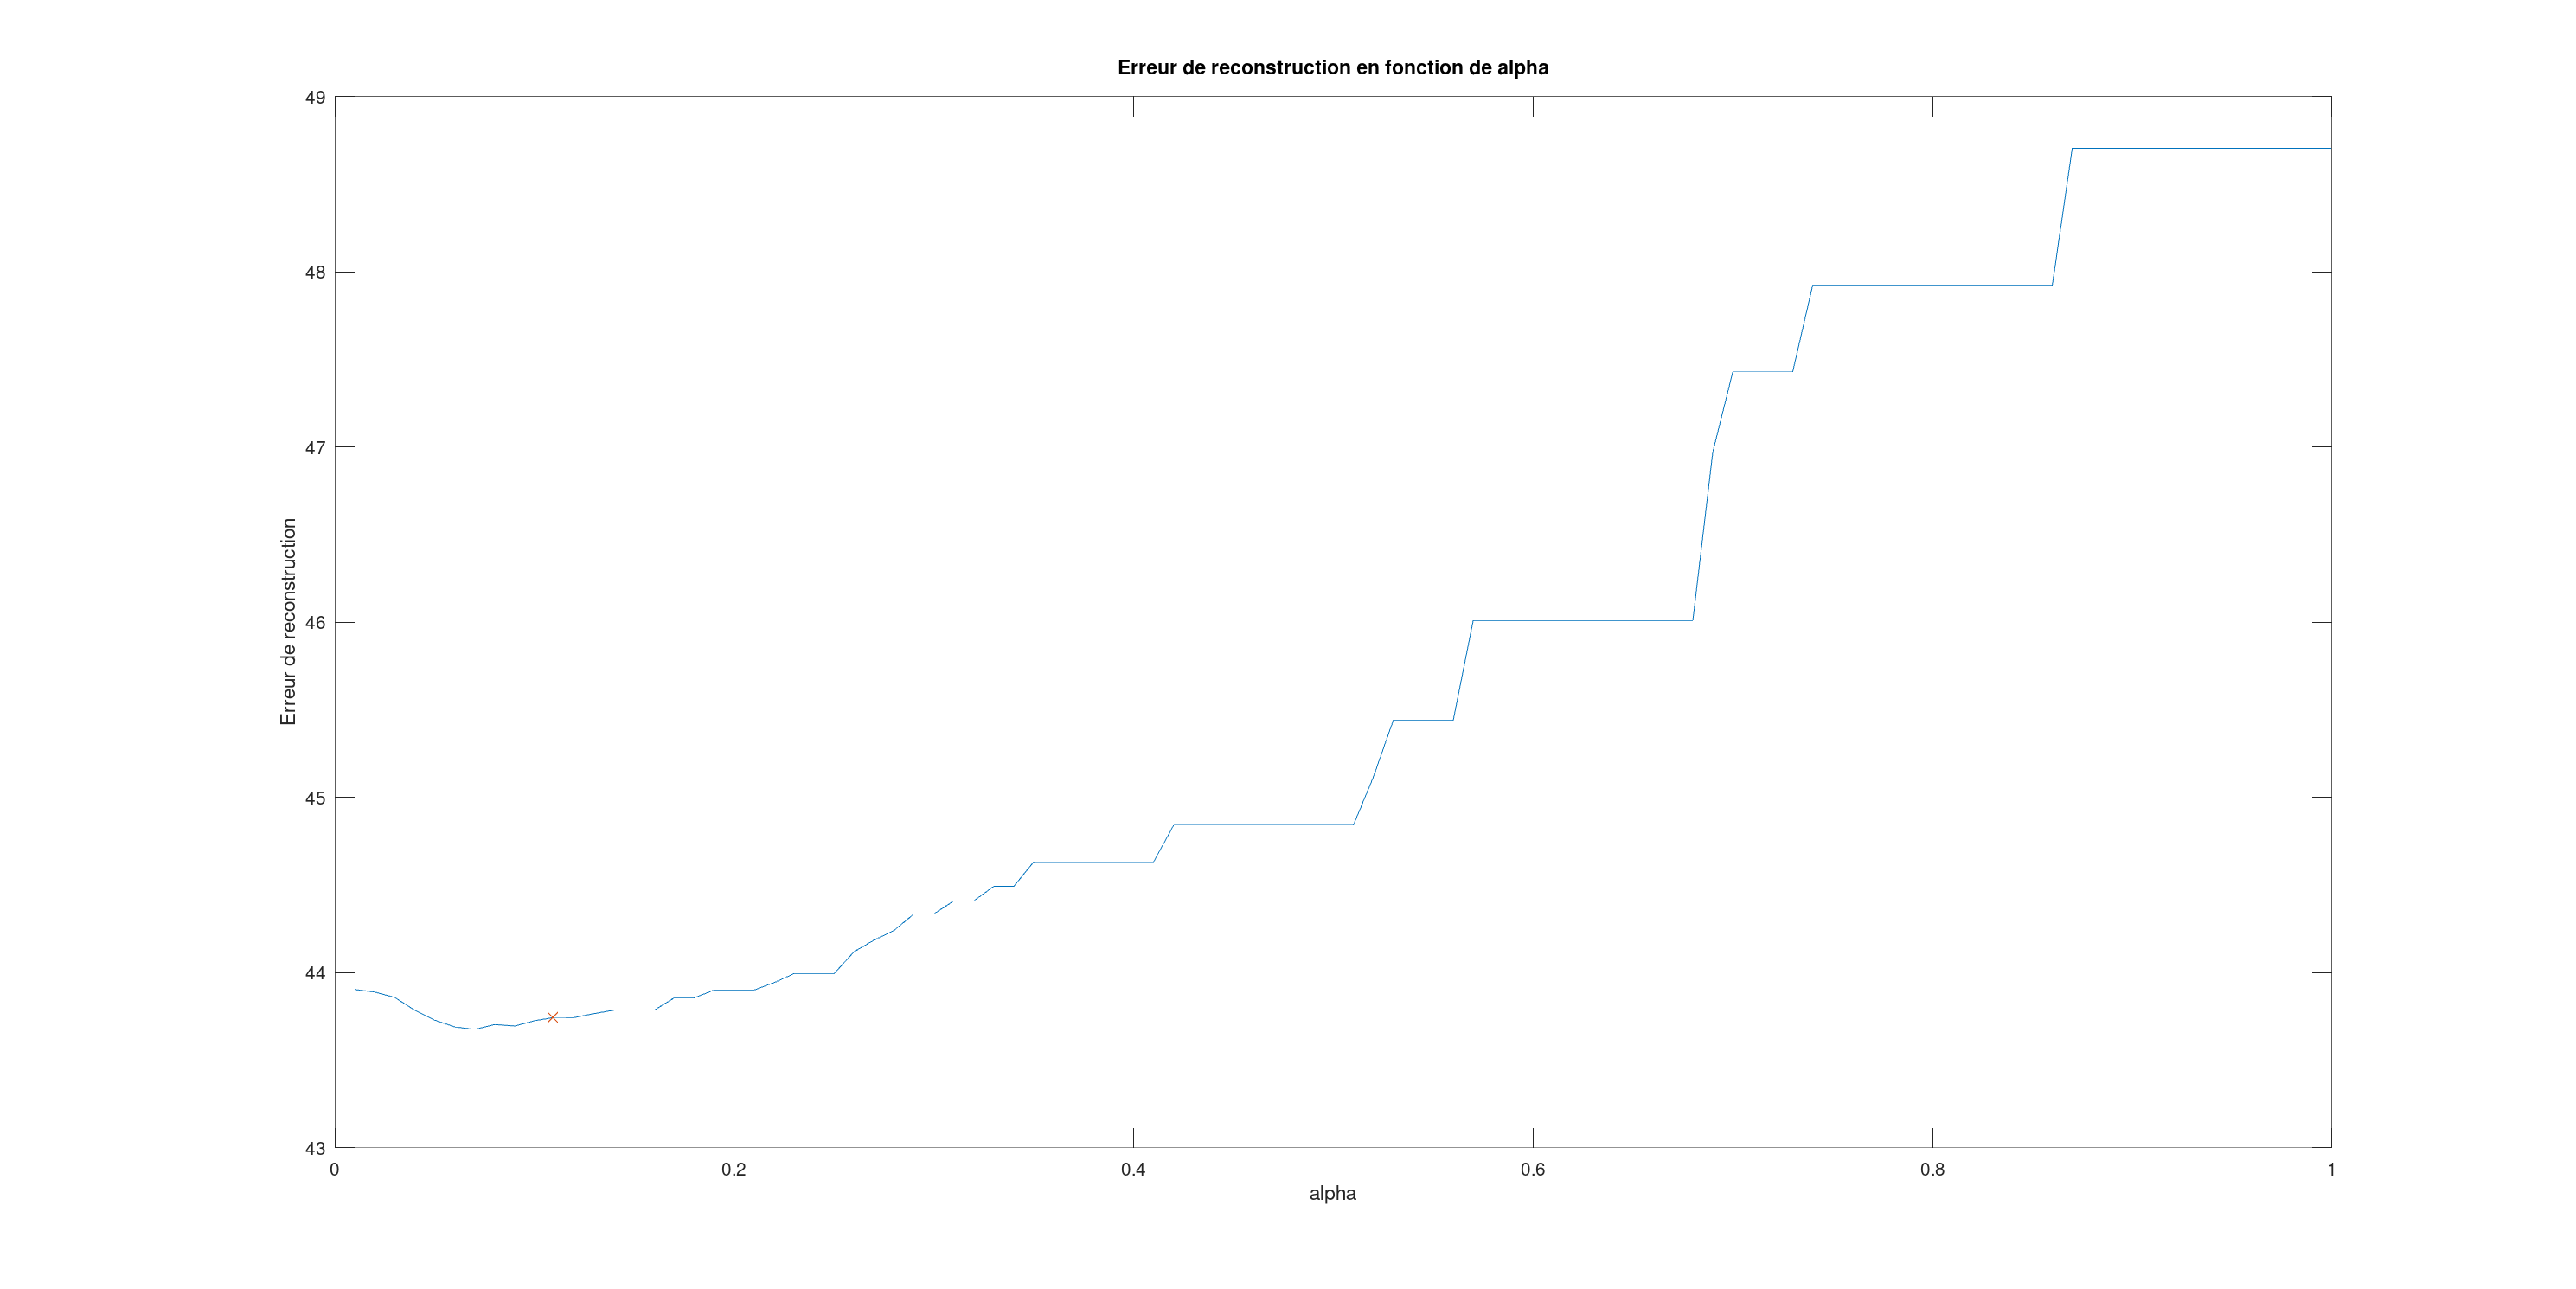
\includegraphics[width=\textwidth]{ex2_7bis}
                    \centering
                \end{figure}

                On remarque ainsi que pour ces deux signaux on obtient de meilleurs résultats
                en terme d'erreur de reconstruction. Cependant, il convient également de comparer
                la forme des signaux obtenus afin de vérifier que le signal reconstruit permet
                aussi de rendre compte des transitions brusques dans le cas du signal "Blocks"
                par exemple.

            }

    \end{enumerate}

    \section{Compression d'images}

    \begin{enumerate}

        \item{On ouvre l'image \texttt{peppers.tiff} à l'aide de la fonction
                \texttt{imread} de Matlab.
            }

        \item{
                Visualisions cette image :

                \begin{figure}[H]
                    \caption{Image \texttt{peppers.tiff}}
                    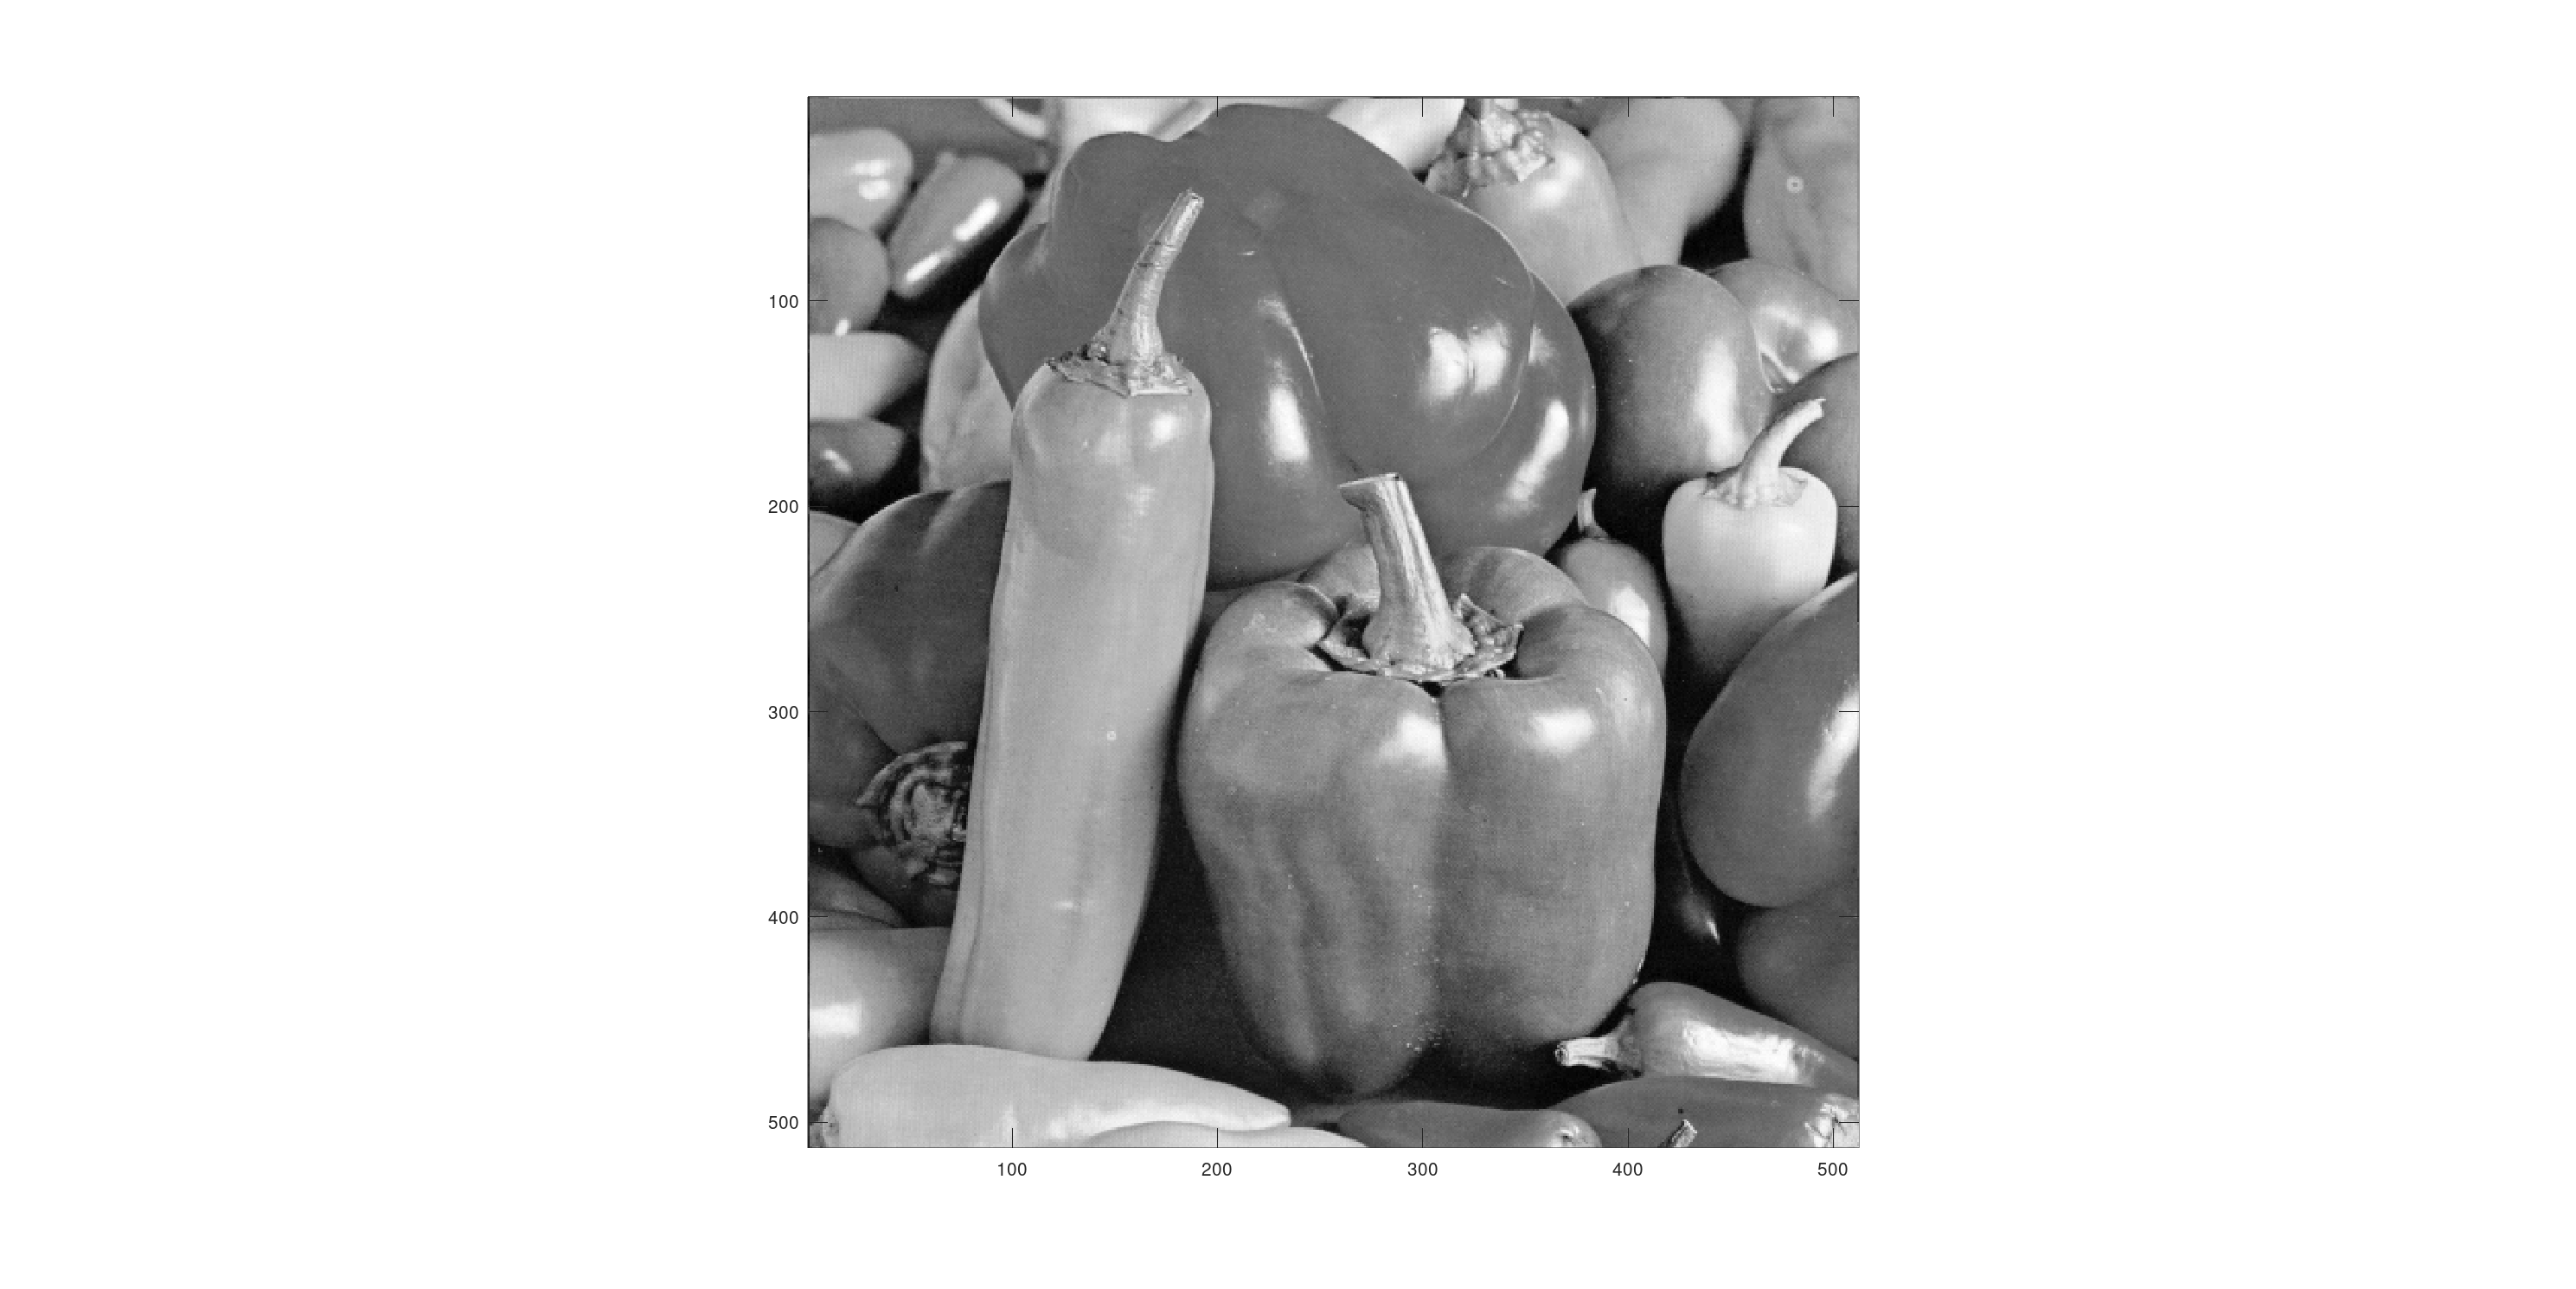
\includegraphics[width=\textwidth]{ex3_1}
                    \centering
                \end{figure}
            }

        \item{On calcule sa transformée en ondelettes 2D à l'échelle J = 4}

        \item{Visualisions alors cette DWT-2D :

                \begin{figure}[H]
                    \caption{DWT-2D}
                    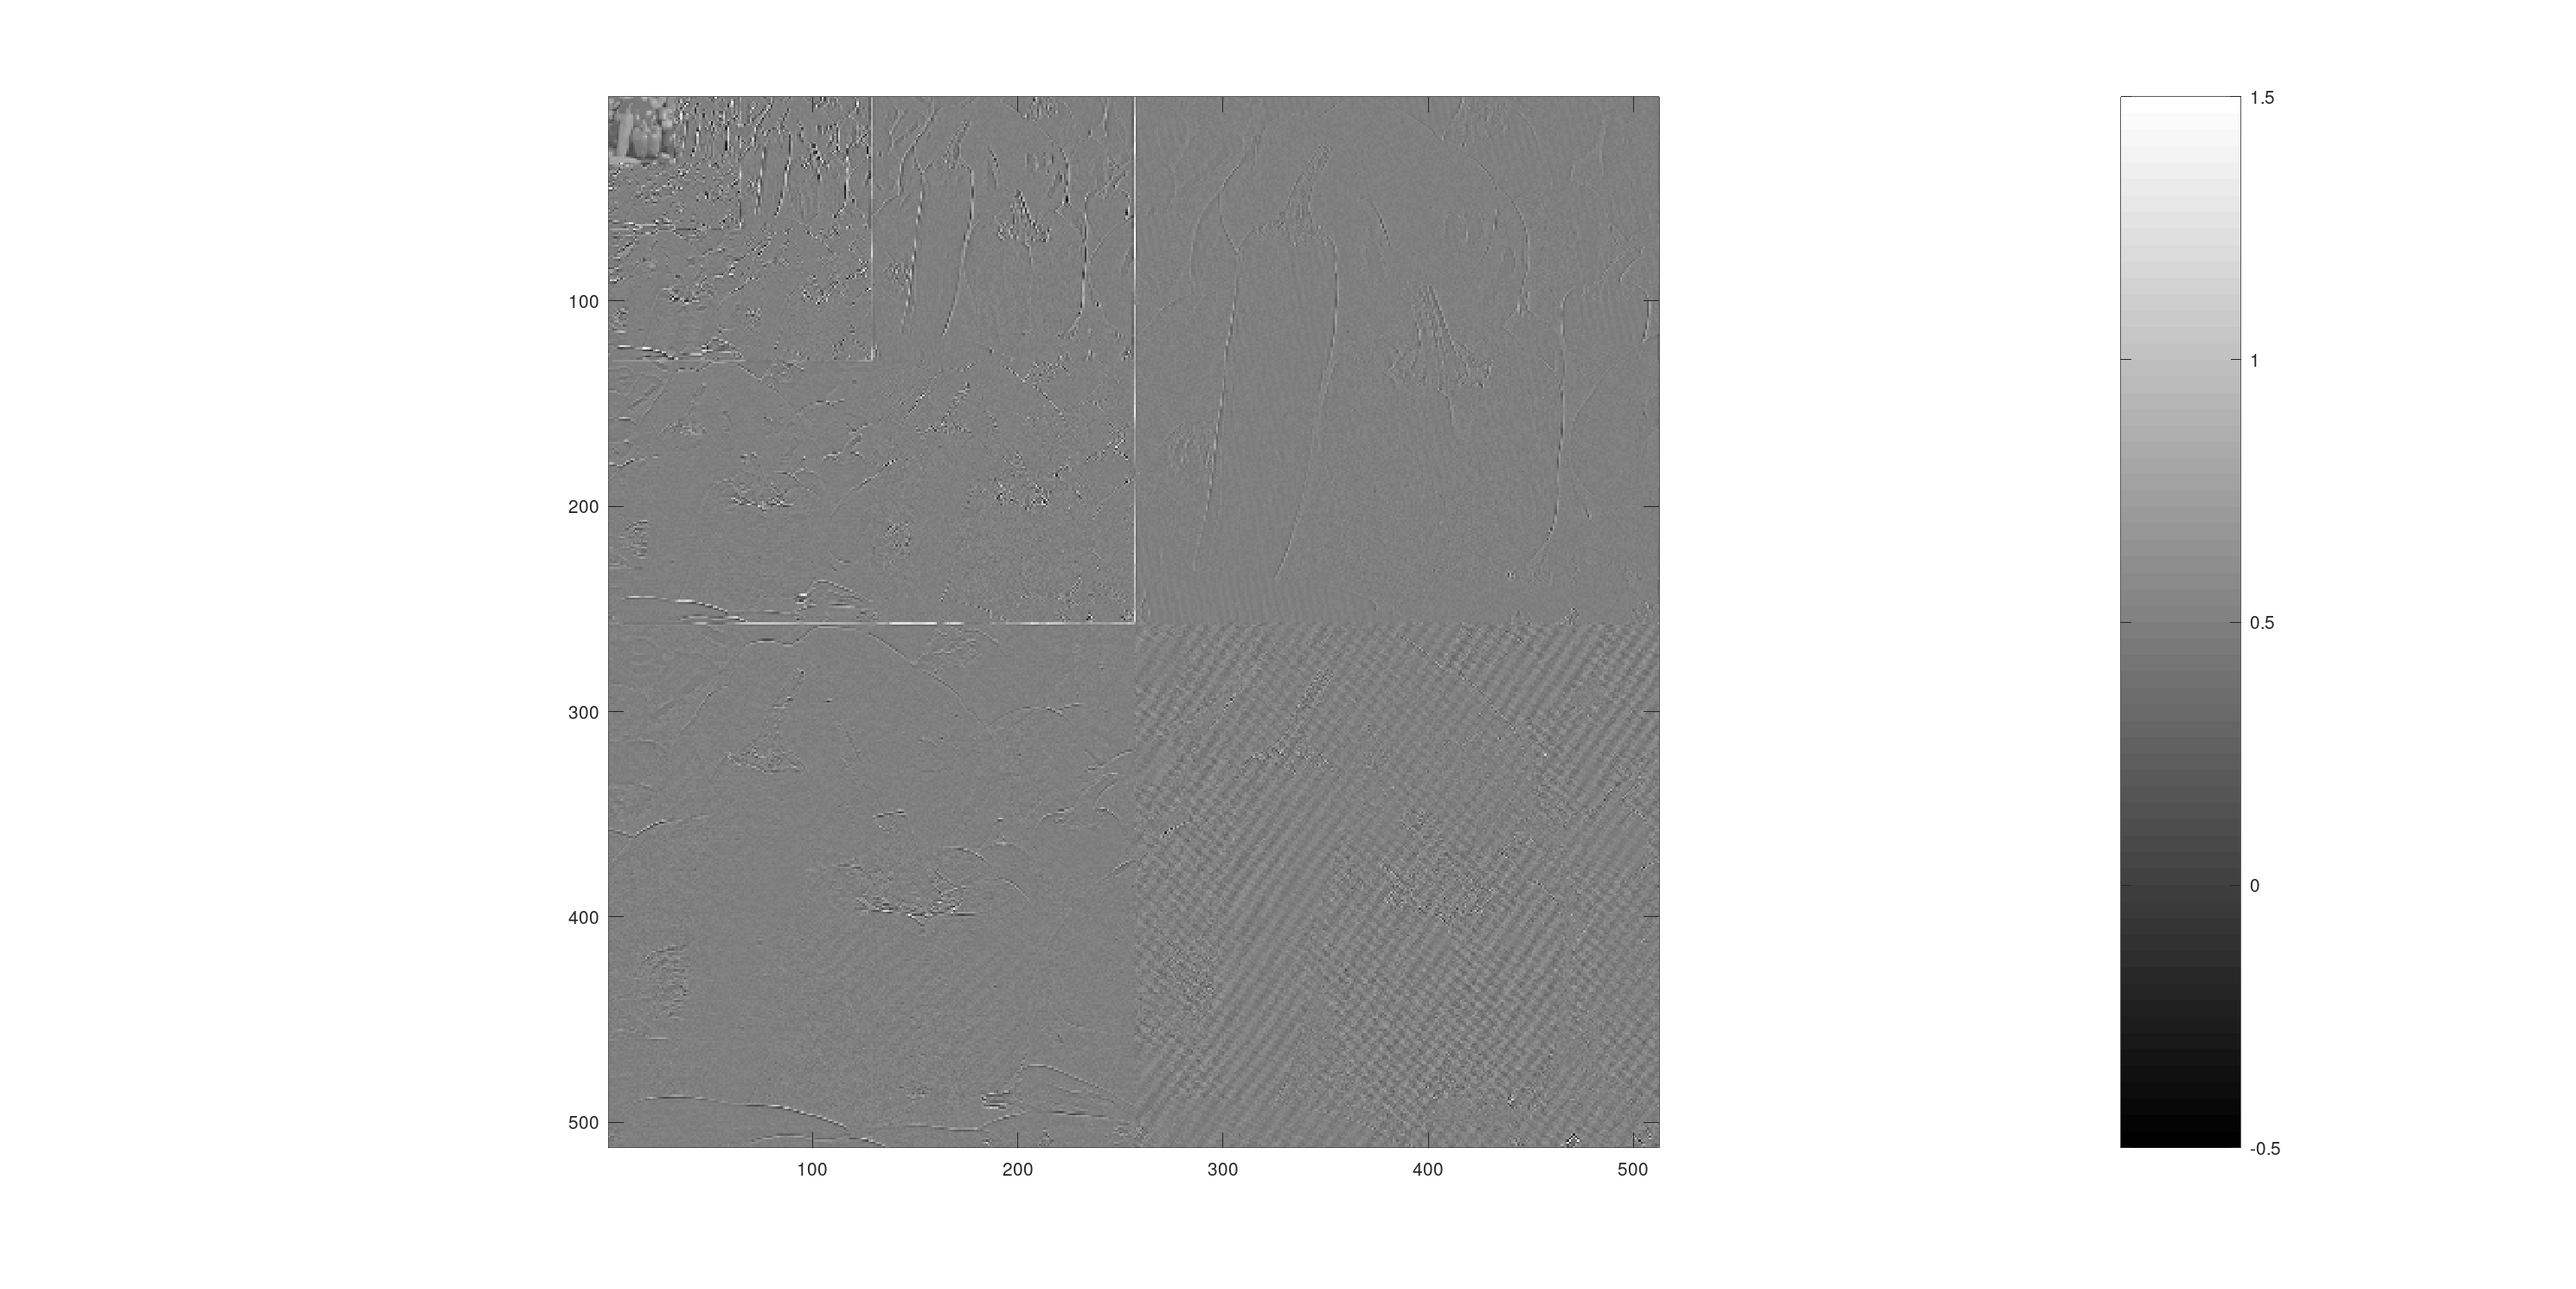
\includegraphics[width=\textwidth]{ex3_2}
                    \centering
                \end{figure}
            }

        \item{Représentons l'histogramme des coefficients et traçons les par
                ordre décroissant en valeur absolue :

                \begin{figure}[H]
                    \caption{Histogramme}
                    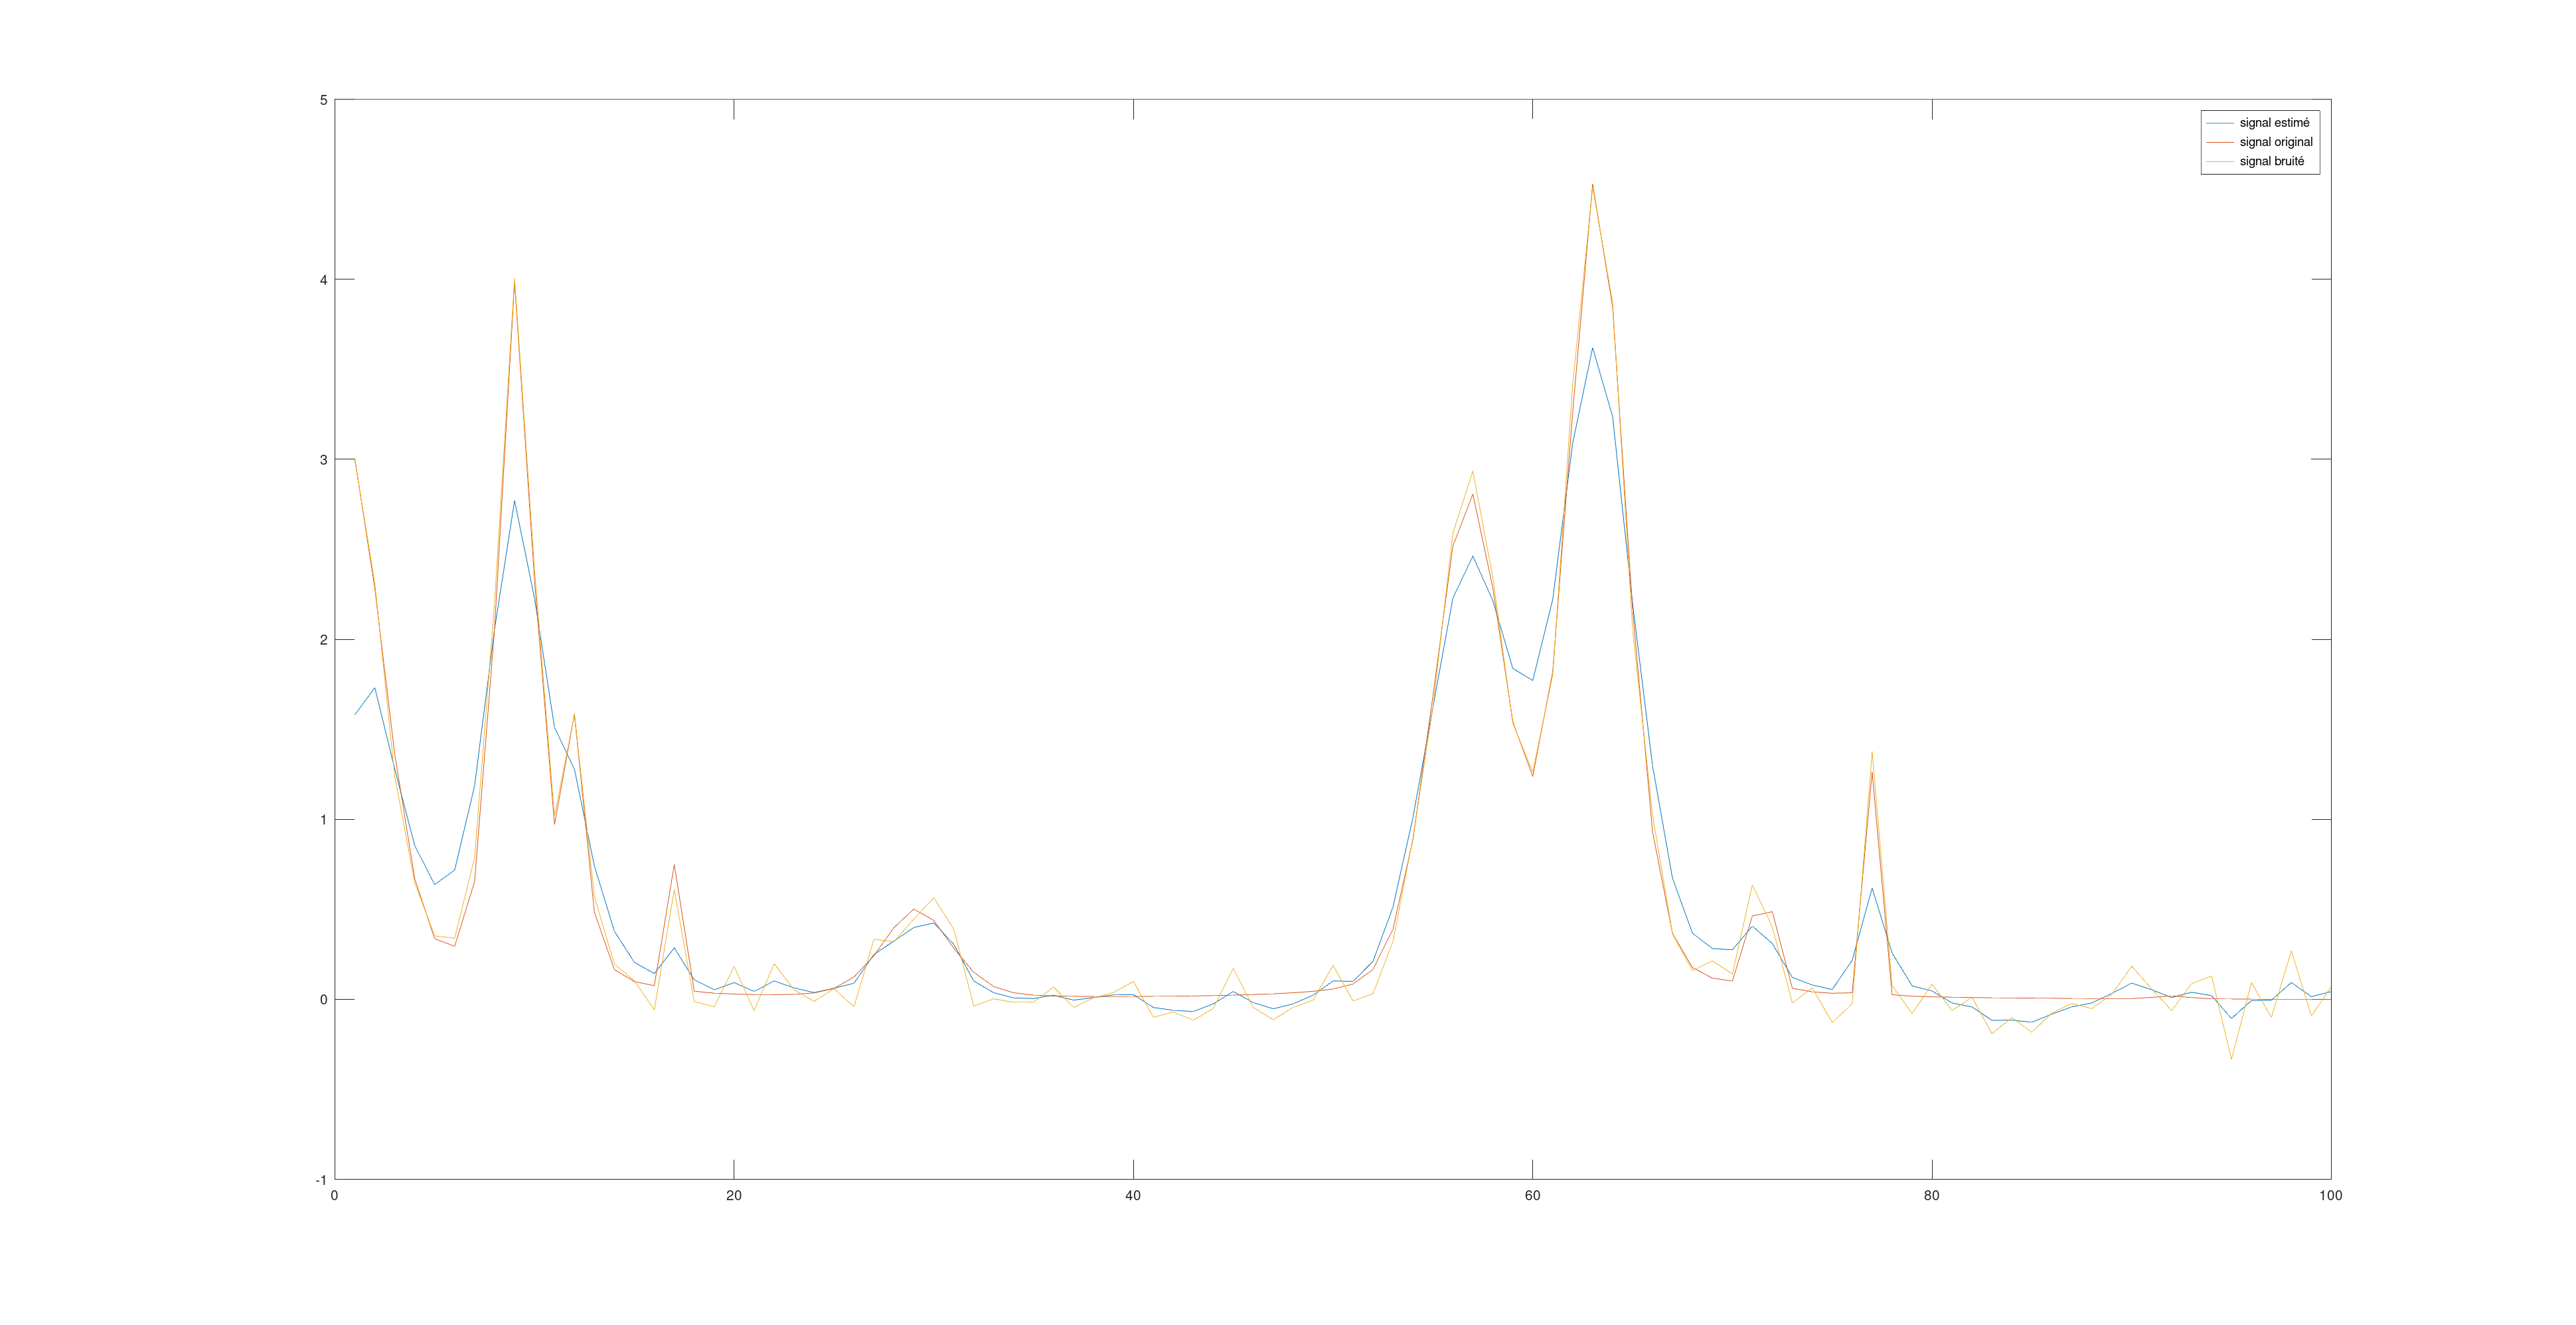
\includegraphics[width=\textwidth]{ex3_3}
                    \centering
                \end{figure}

                \begin{figure}[H]
                    \caption{coefficients (ordre décroissant)}
                    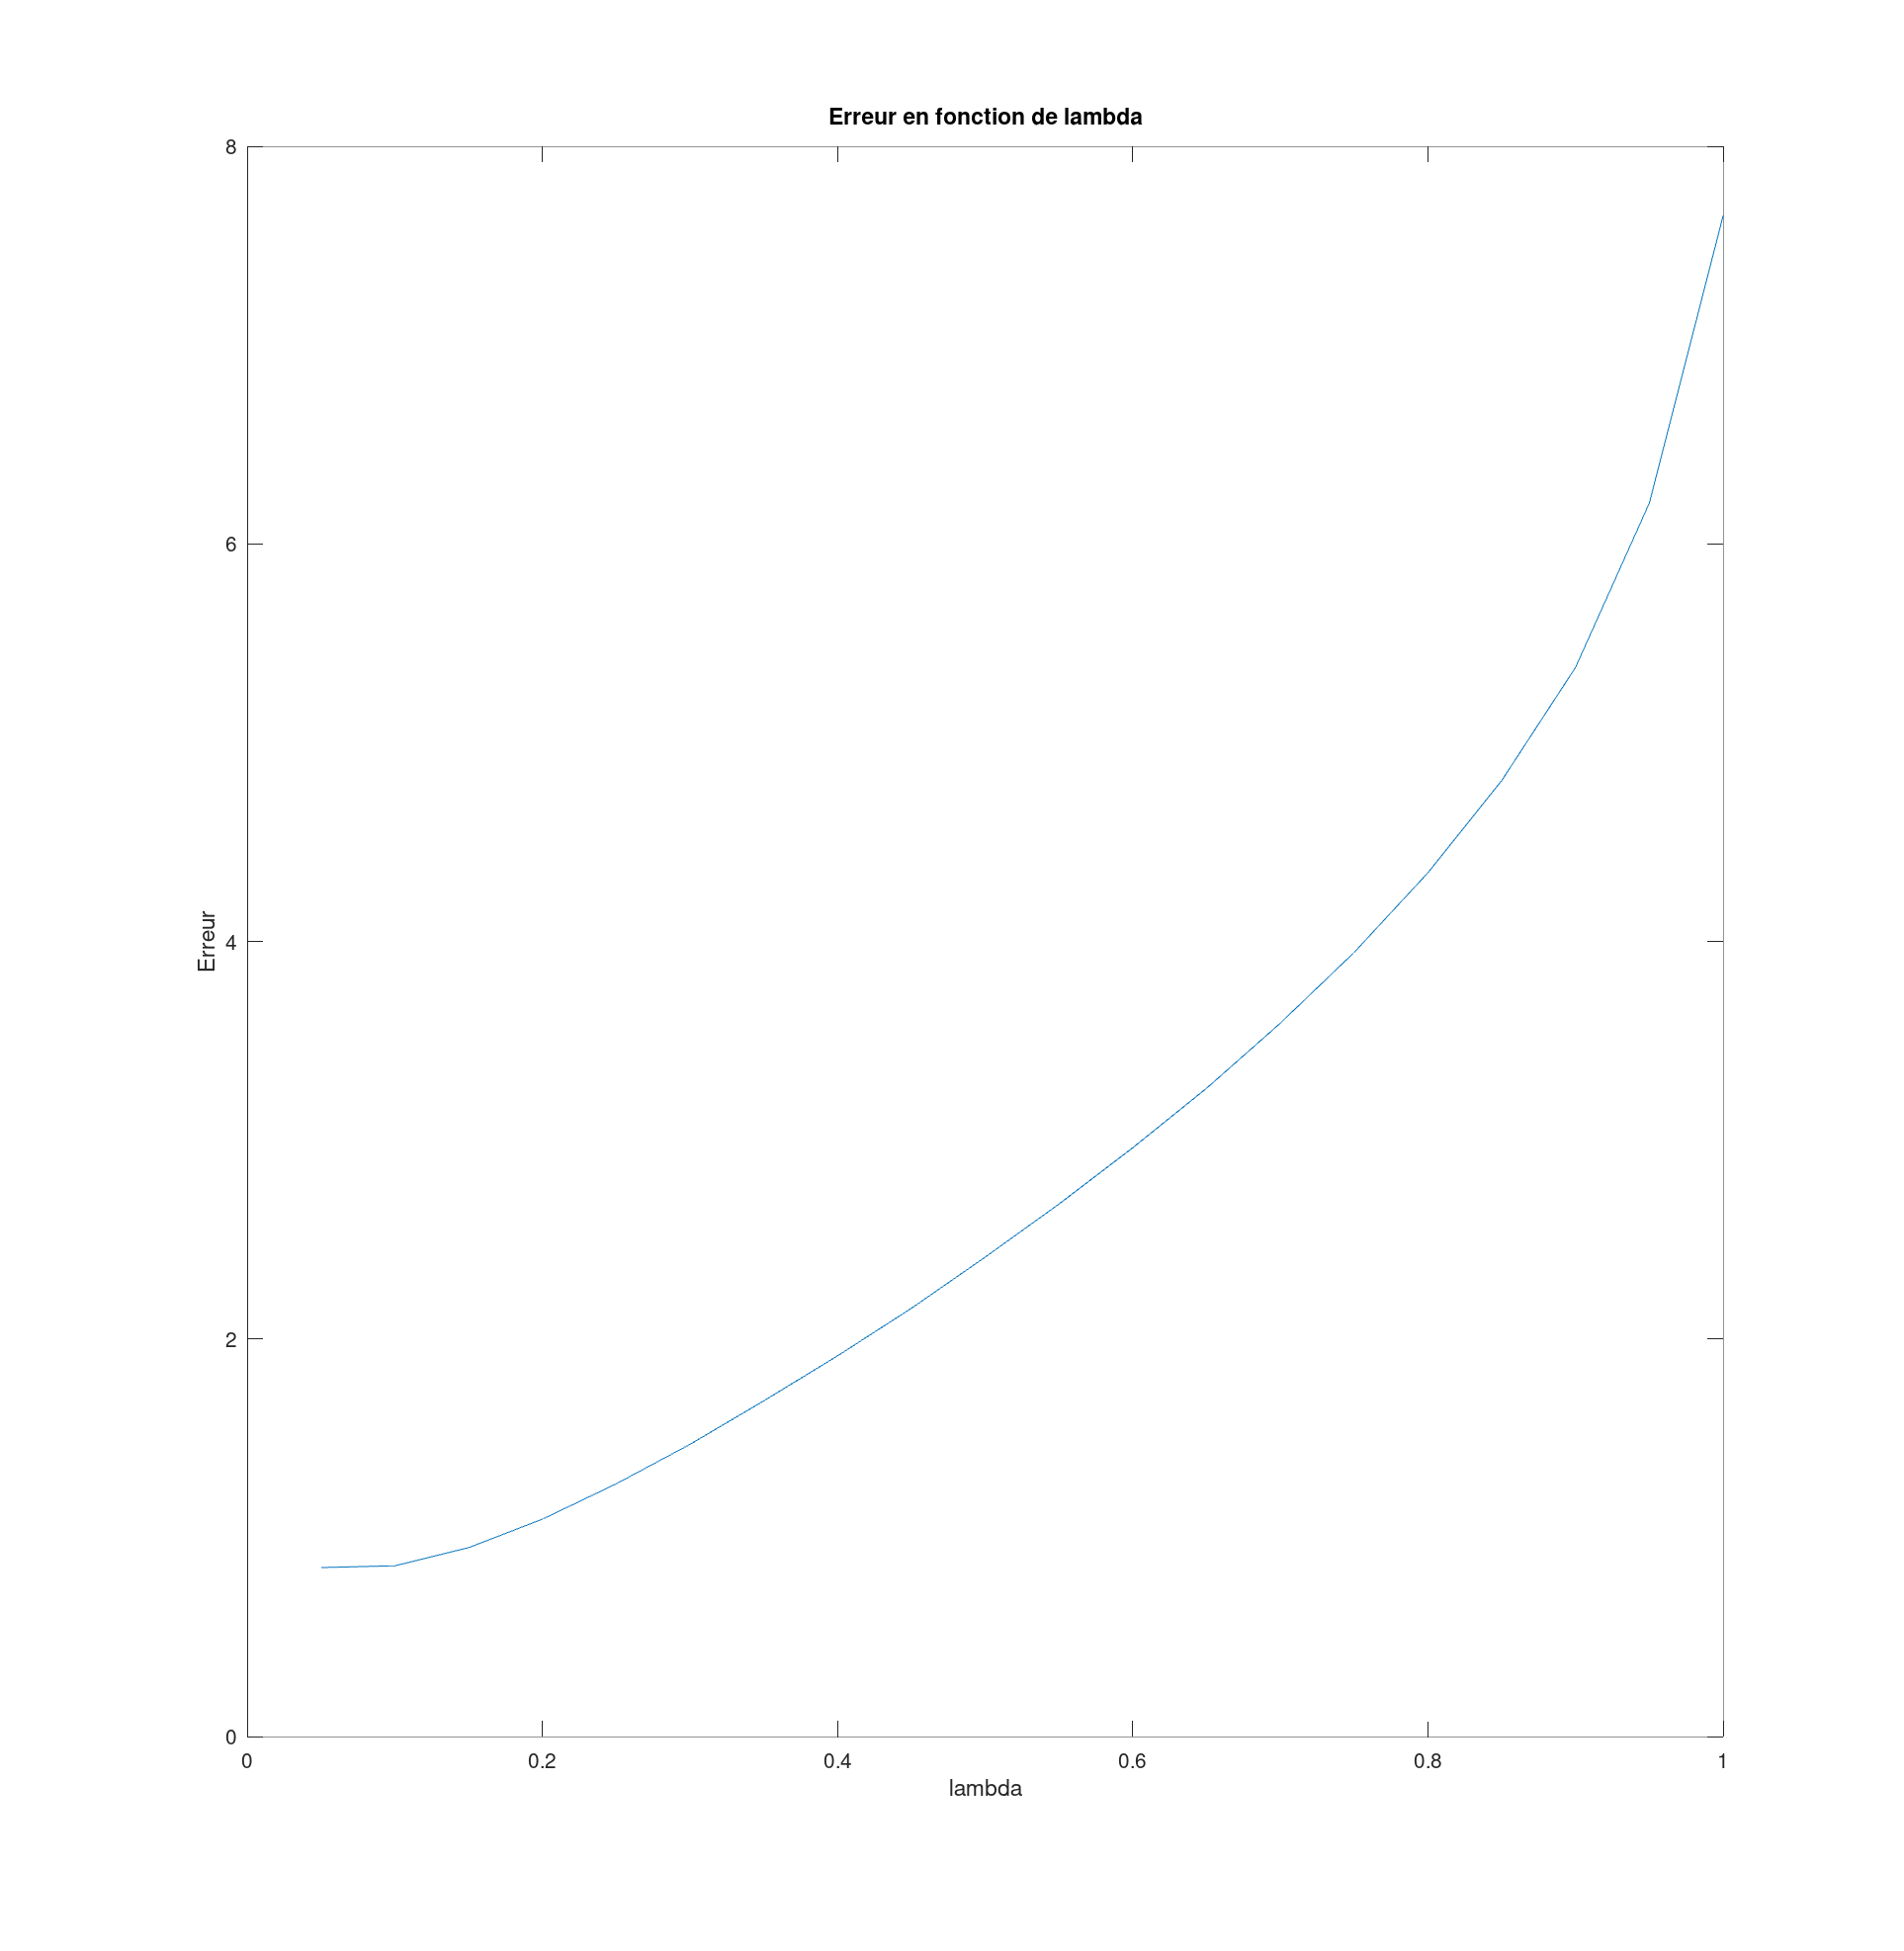
\includegraphics[width=\textwidth]{ex3_4}
                    \centering
                \end{figure}

                On remarque que cet histogramme contient beaucoup plus de valeurs faibles que
                de valeurs élevées et s'apparente à une gaussienne de variance faible.

            }

        \item{{La procédure de compression consiste en la reconstruction de l'image à partir de sa DWT
                seuillée. On se donne un $\tau$ et on ne conserve que les $\tau \%$ coefficients
                les plus grands.
            }

        \item{Visualisions l'image reconstruite pour $\tau \in \{1,5,20\}$.

                \begin{figure}[H]
                    \caption{Résultats pour $\tau = 1\%$}
                    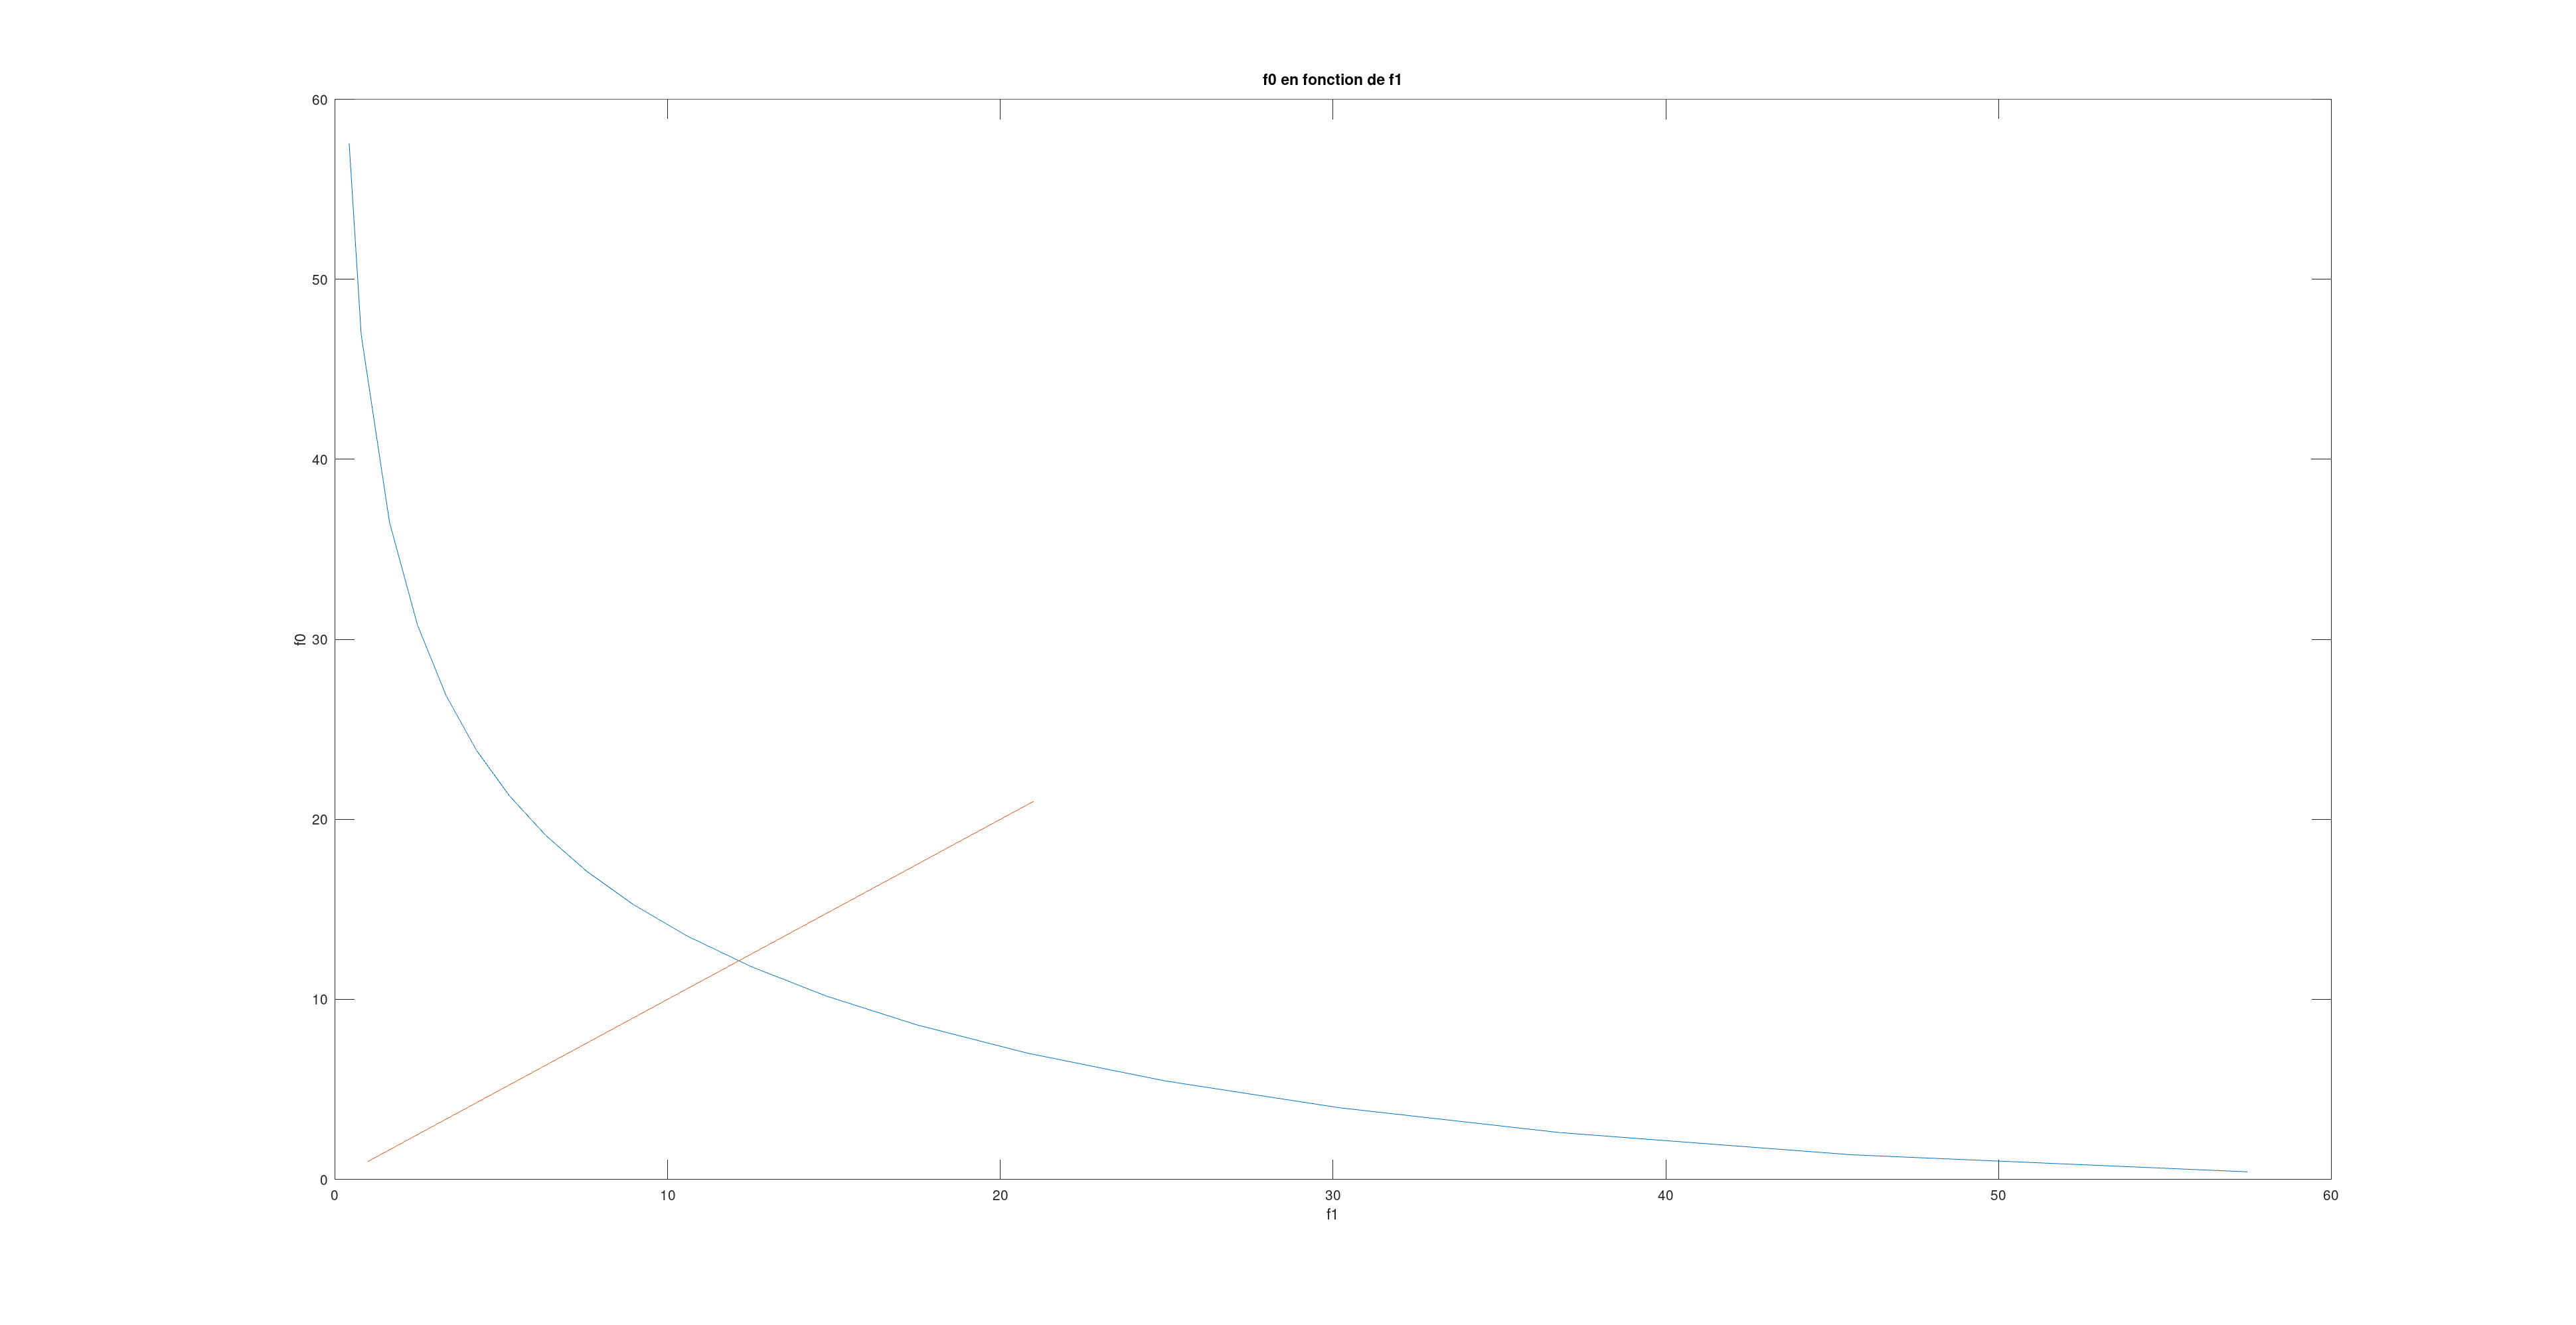
\includegraphics[width=\textwidth]{ex3_5}
                    \centering
                \end{figure}

                \begin{figure}[H]
                    \caption{Résultats pour $\tau = 5\%$}
                    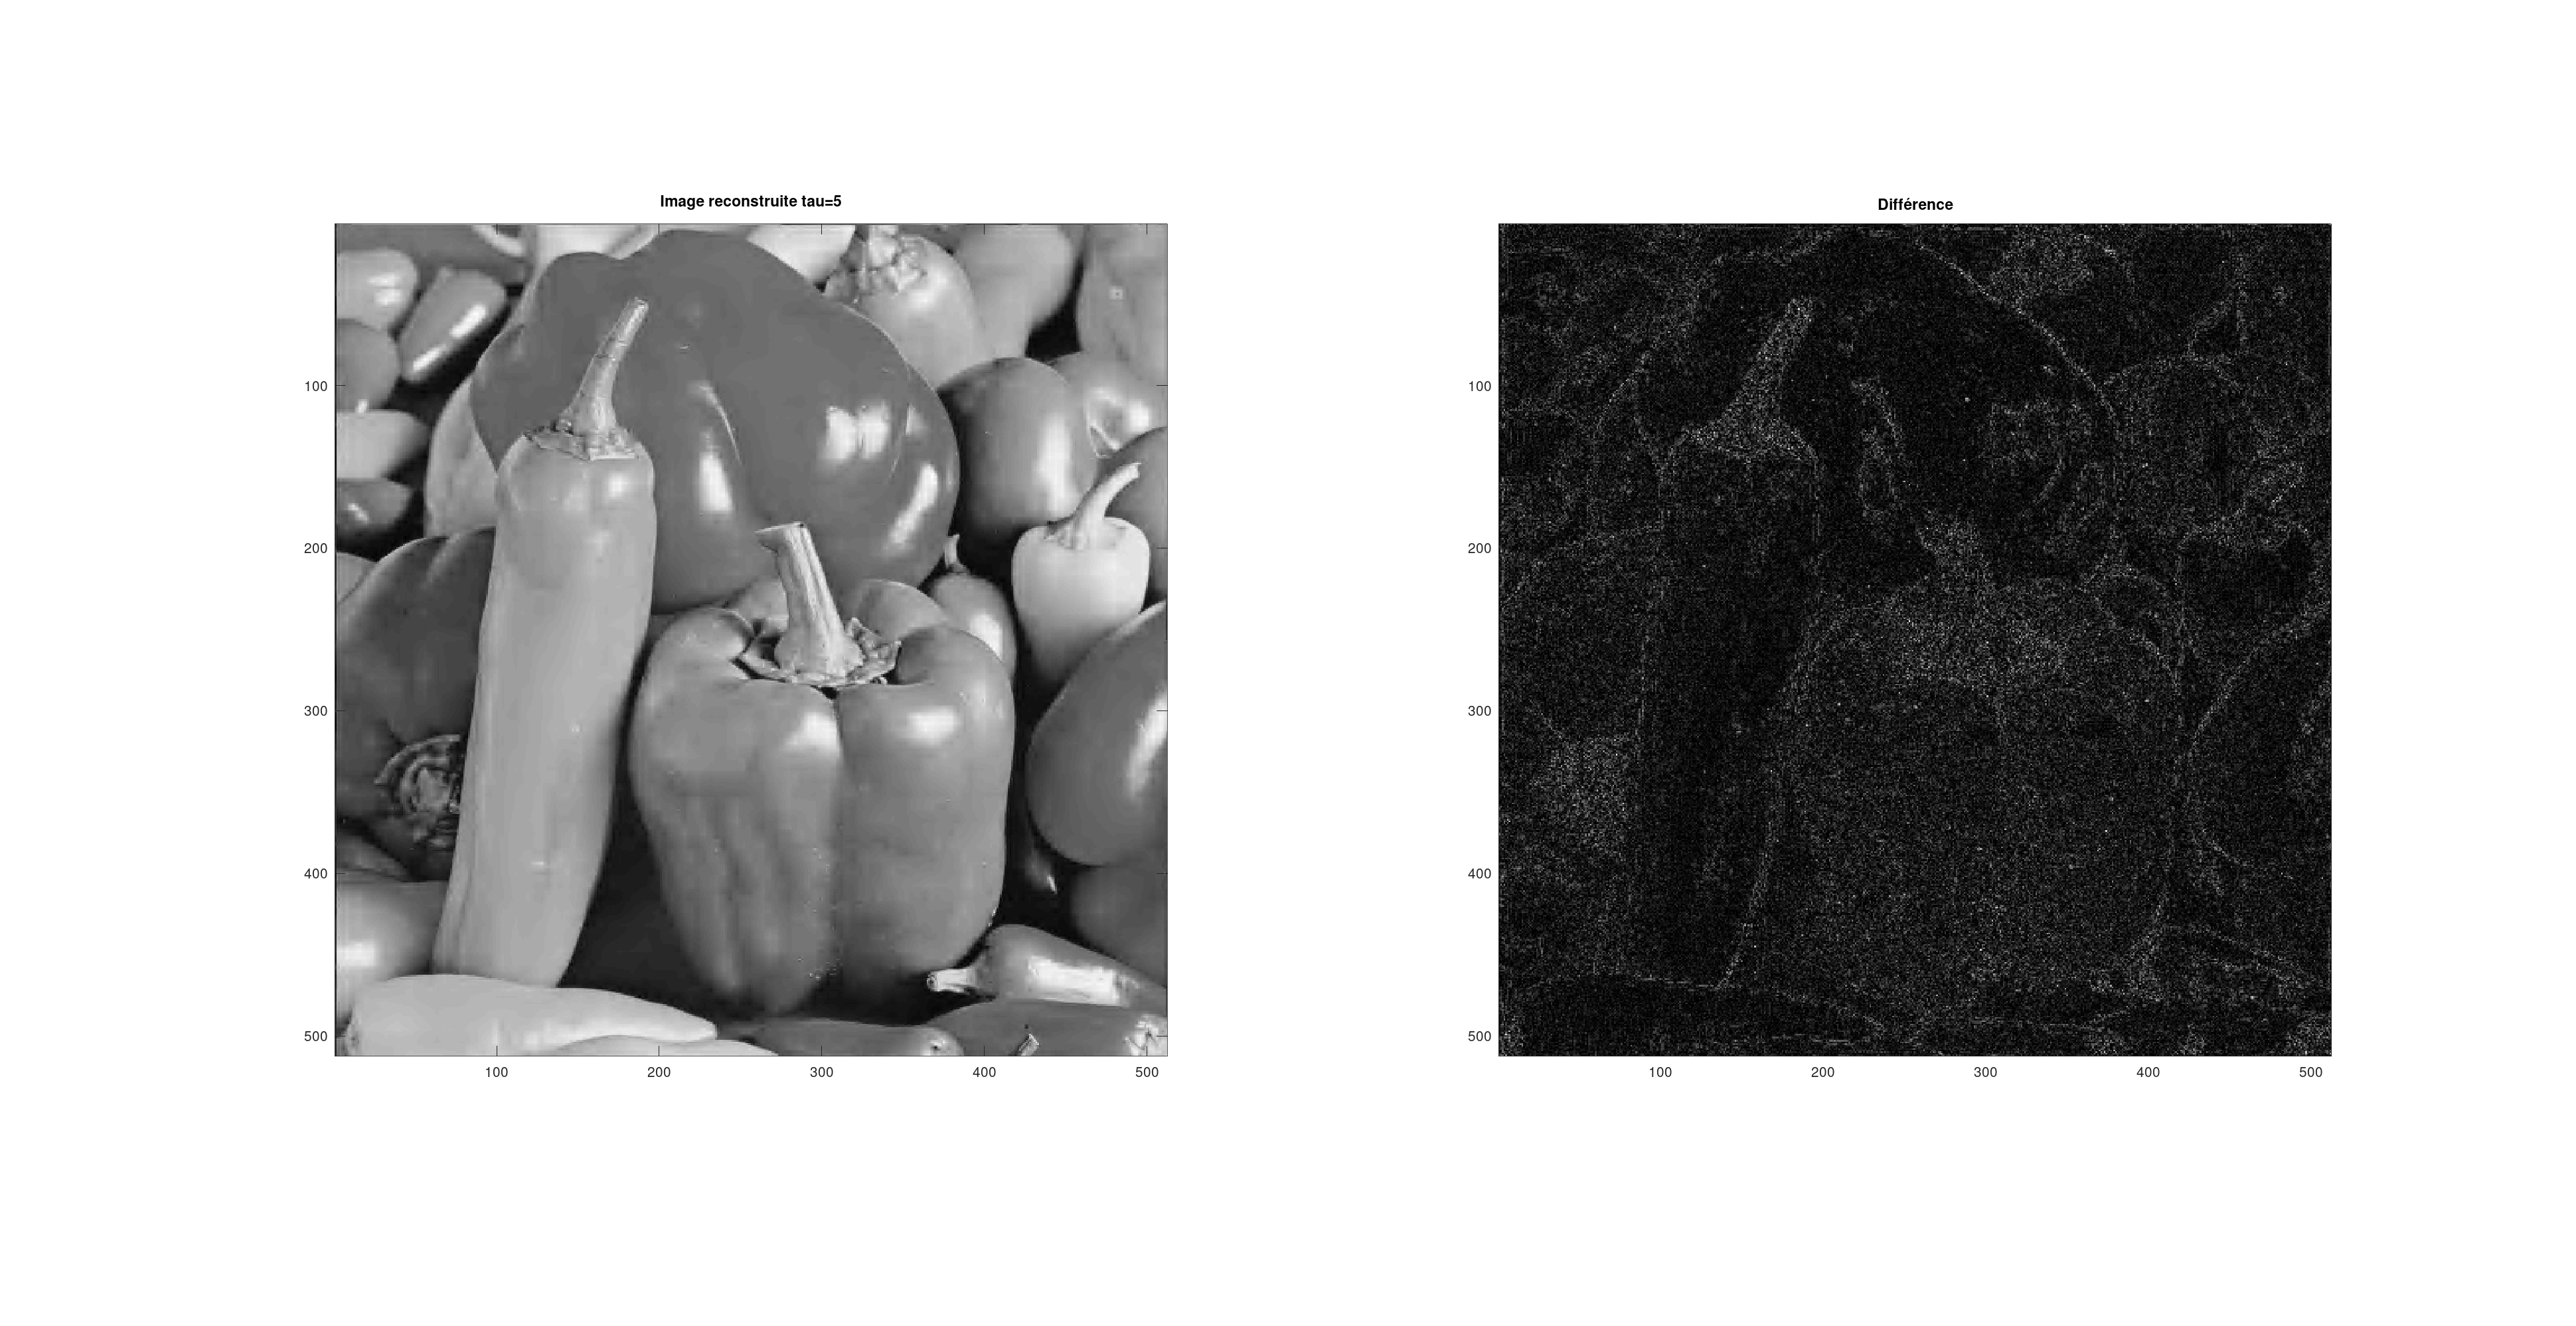
\includegraphics[width=\textwidth]{ex3_6}
                    \centering
                \end{figure}

                \begin{figure}[H]
                    \caption{Résultats pour $\tau = 20\%$}
                    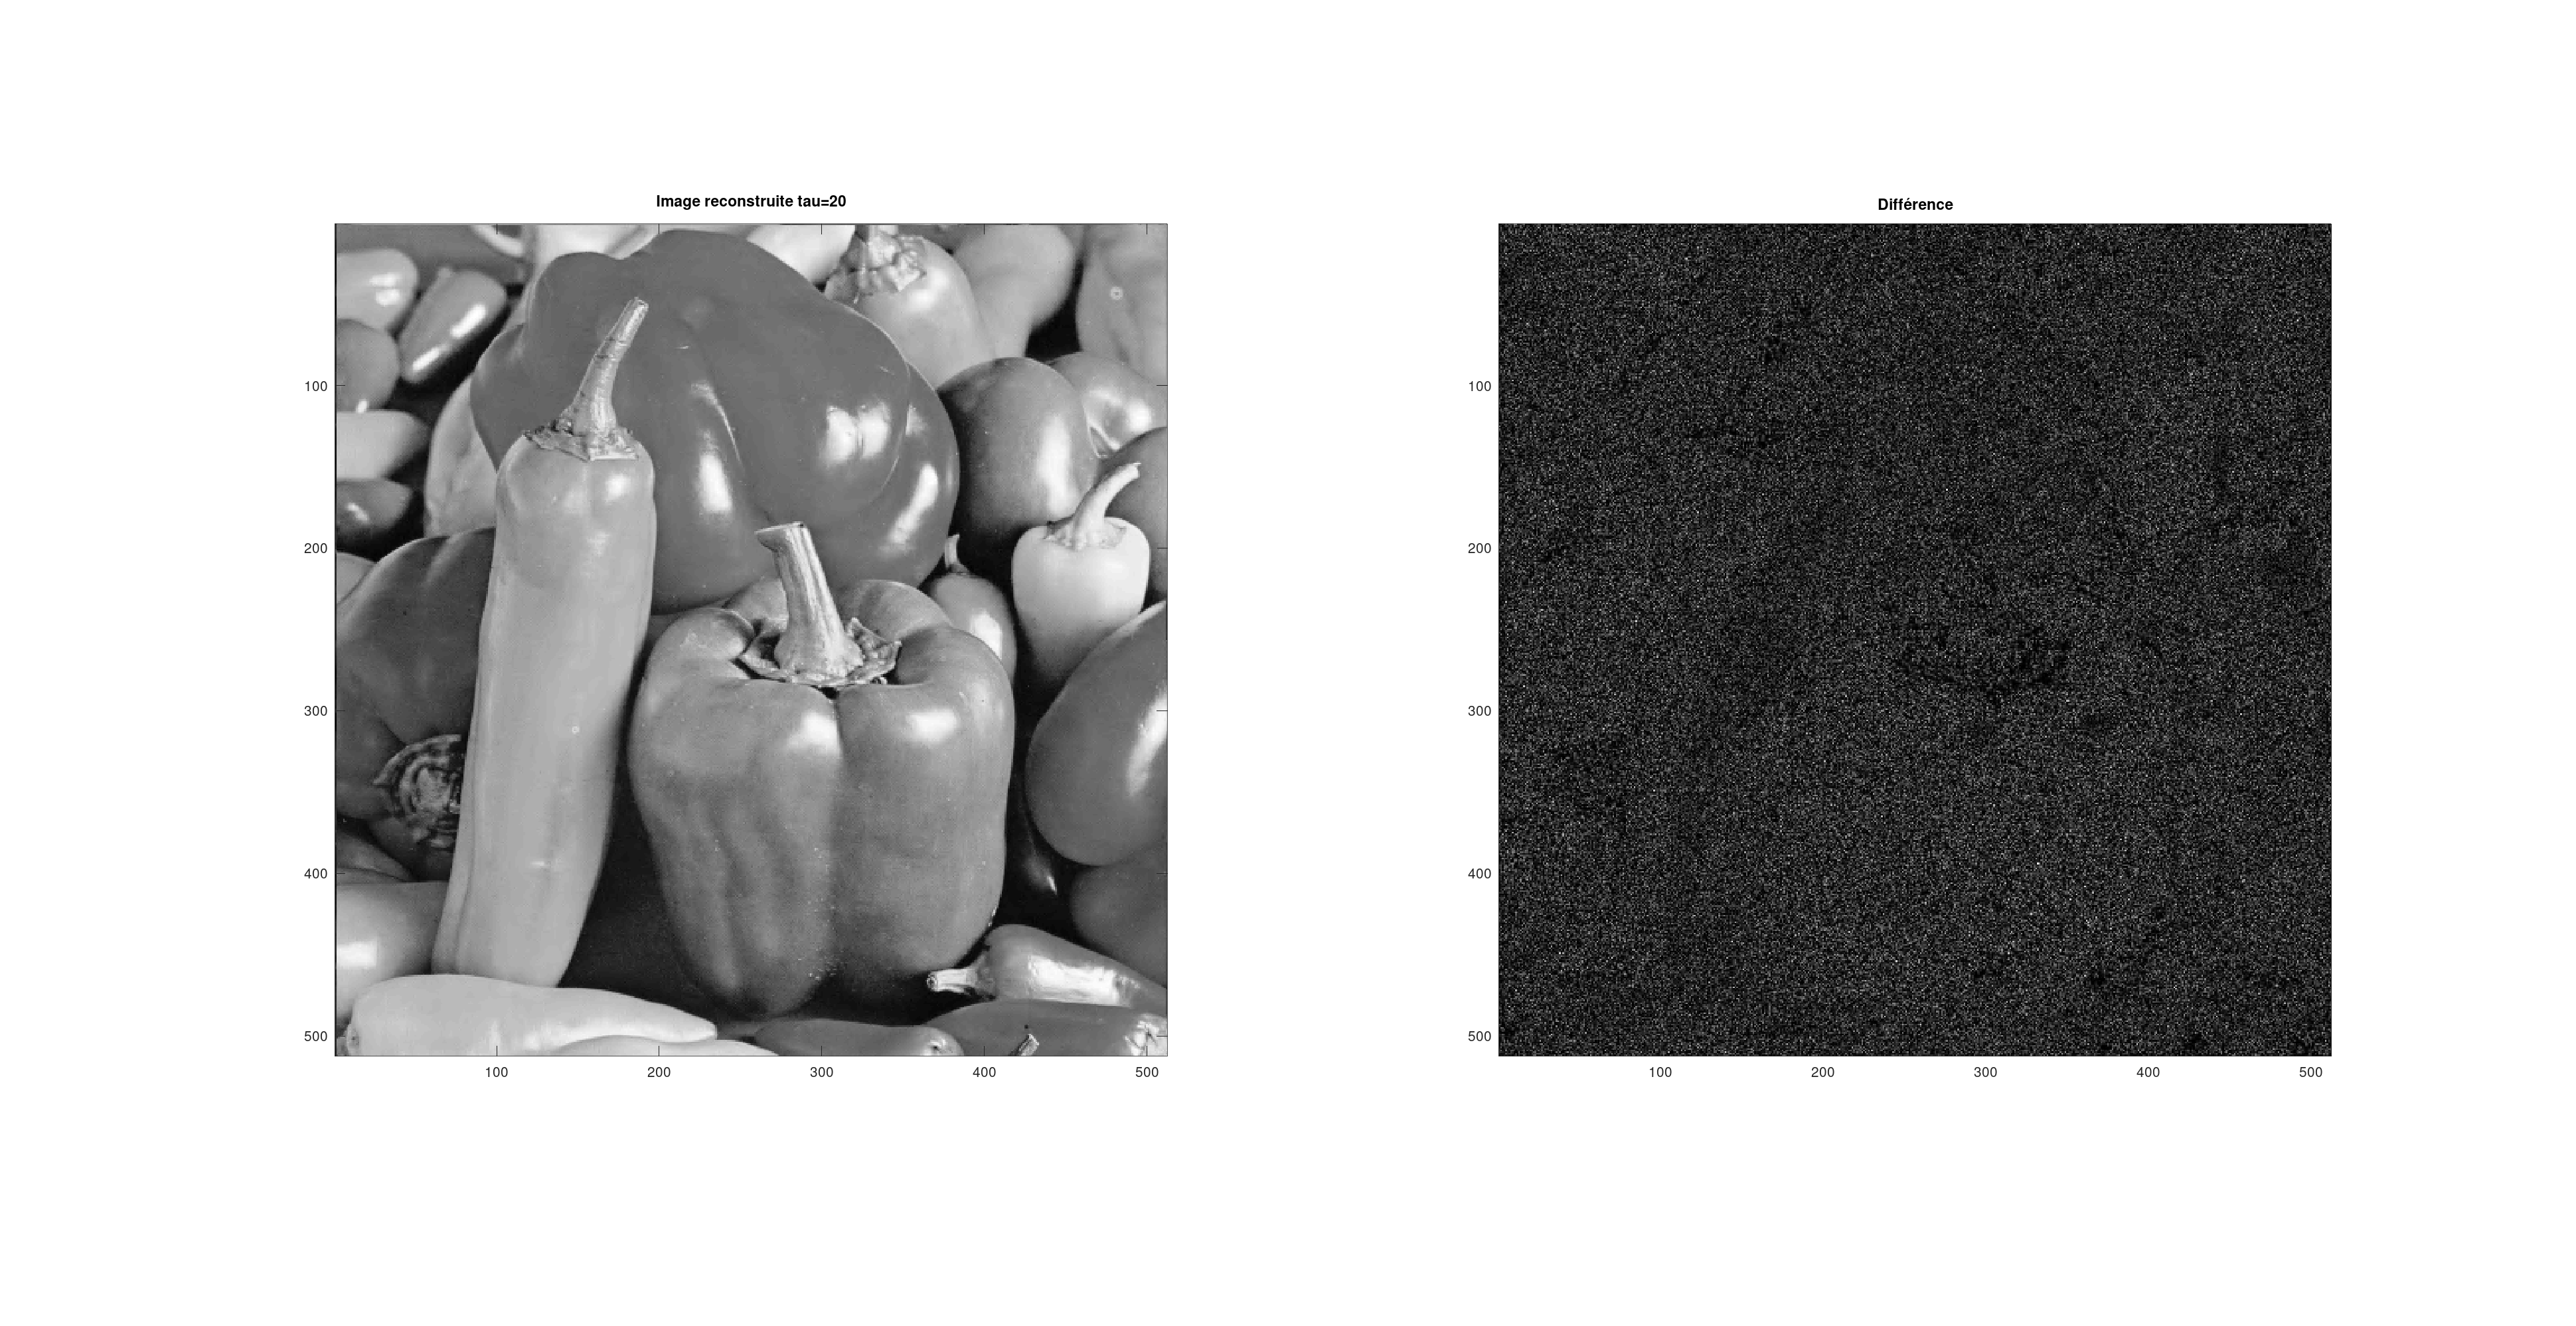
\includegraphics[width=\textwidth]{ex3_7}
                    \centering
                \end{figure}

                On remarque alors que cette procédure de compression permet déjà de reconnaitre
                l'image avec $\tau = 1\%$. Pour $\tau = 20\%$, l'image "différence" n'est pas
                exactement nulle mais conserver par exemple $20\%$ des coefficients suffit à
                obtenir une image quasiment identique à l'originale.
            }

        \item{Avec une ondelette de Haar, on obtient les images suivantes :

                \begin{figure}[H]
                    \caption{Résultats pour $\tau = 1\%$}
                    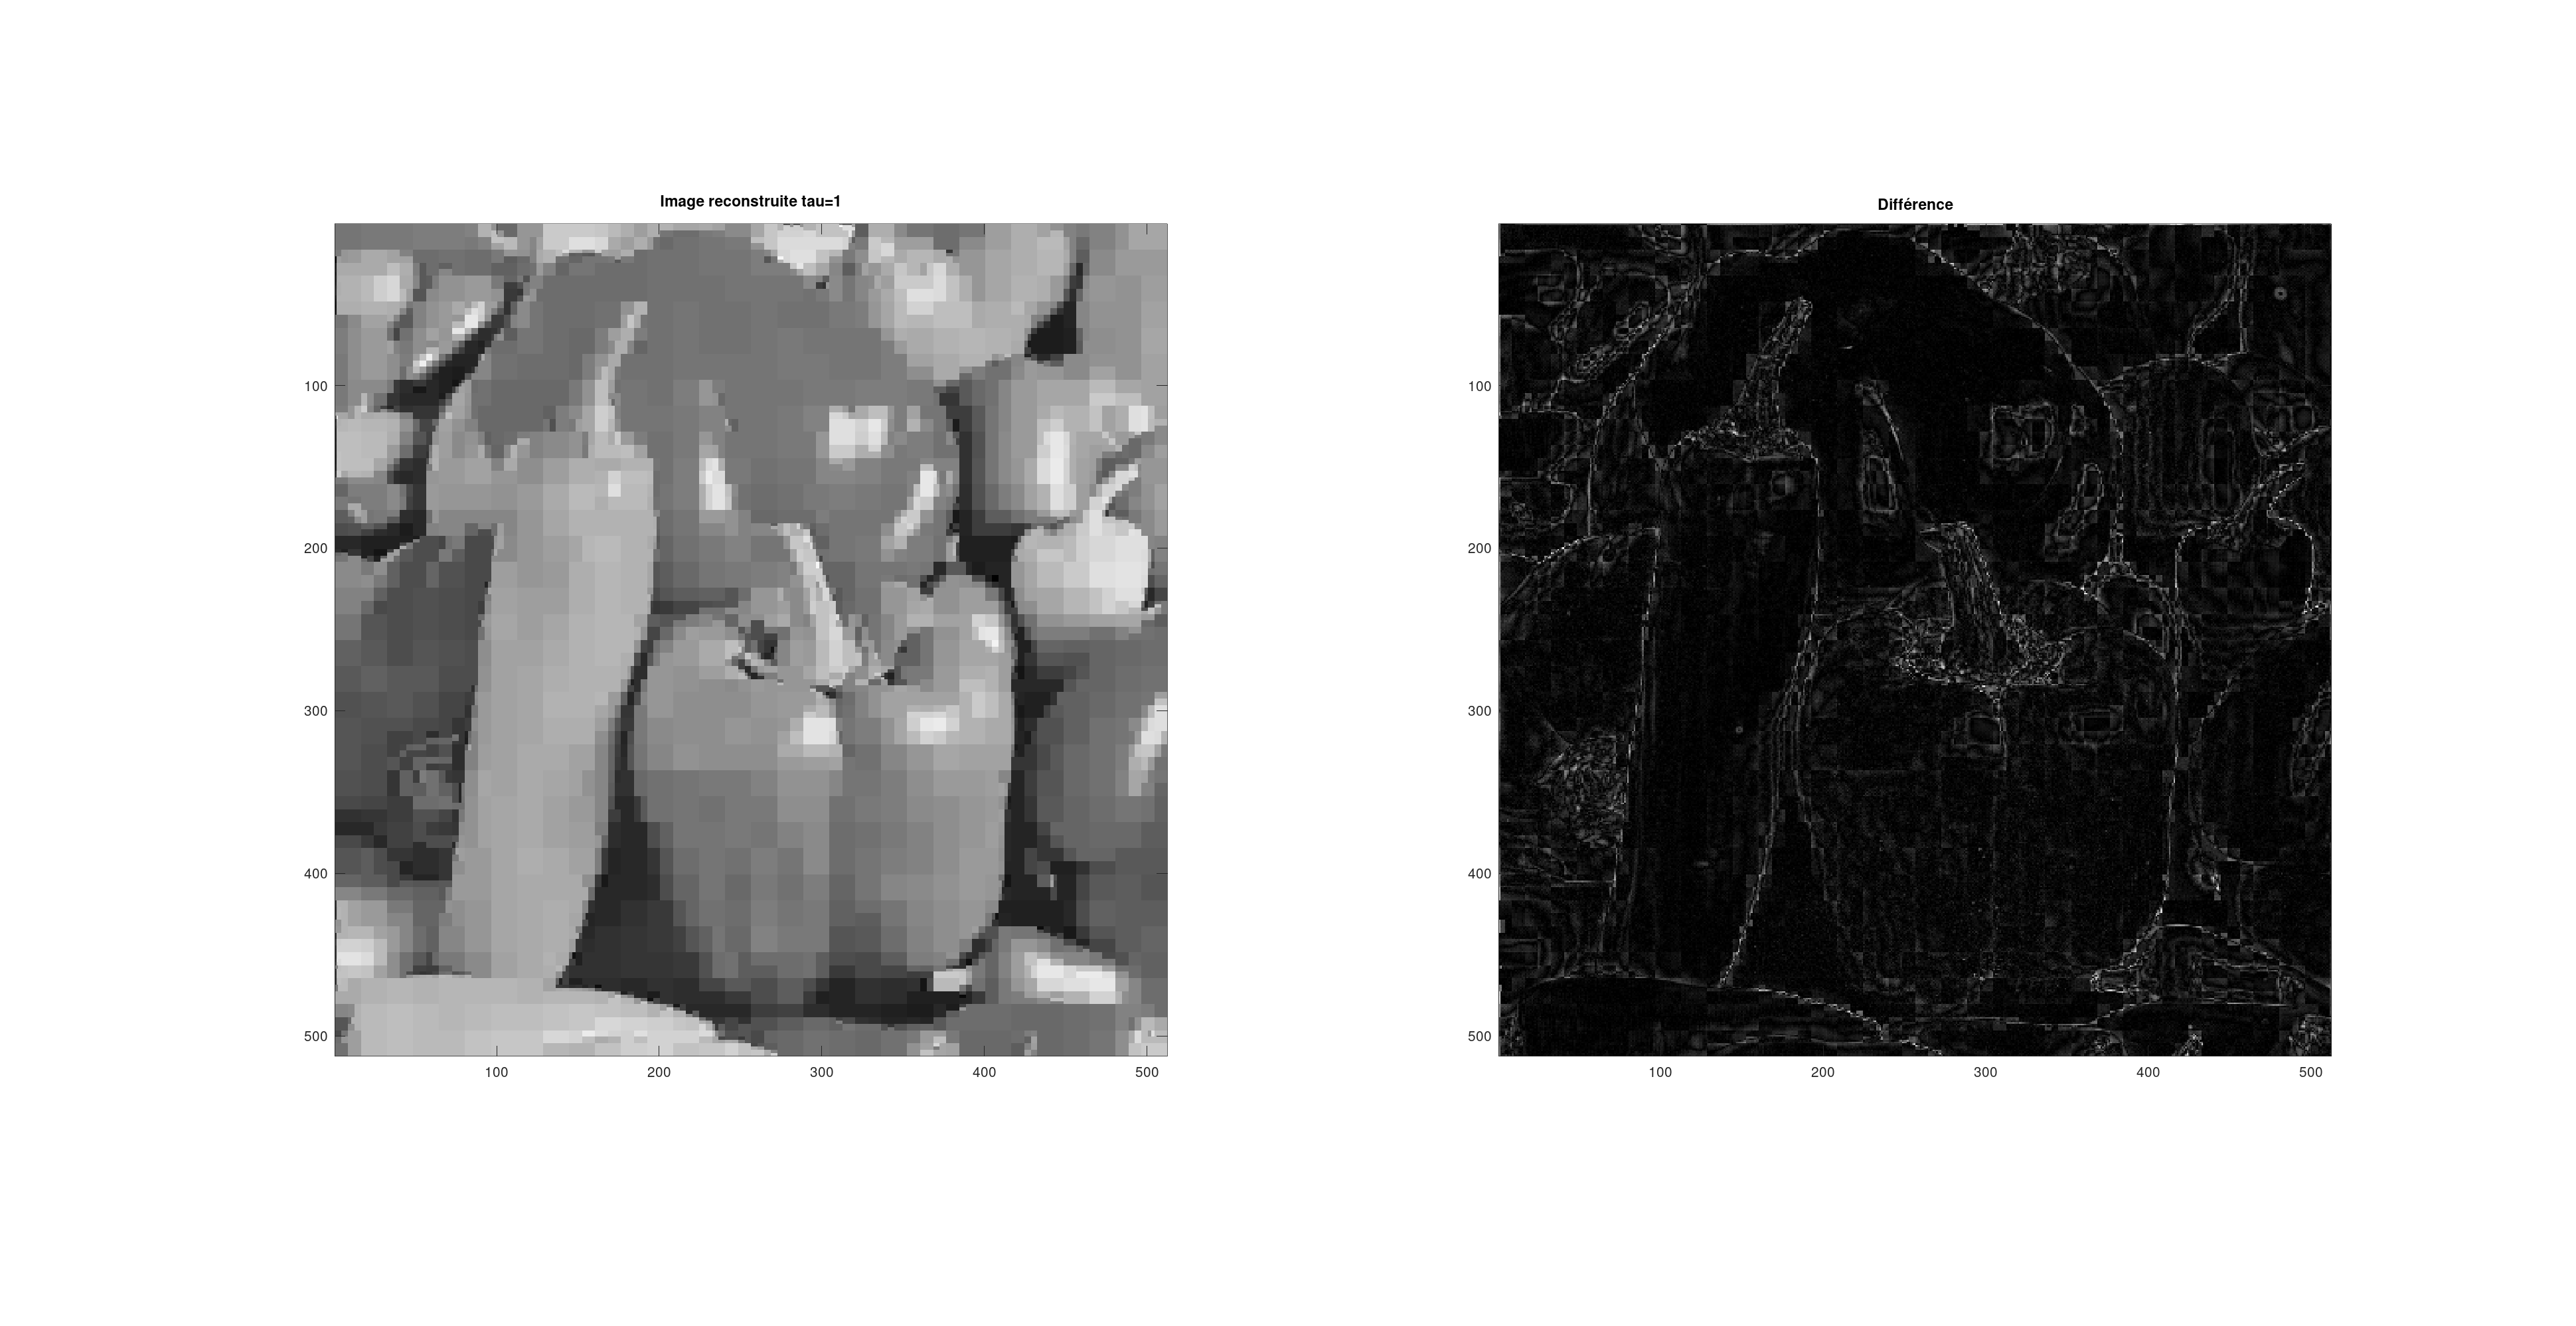
\includegraphics[width=\textwidth]{ex3_8}
                    \centering
                \end{figure}

                \begin{figure}[H]
                    \caption{Résultats pour $\tau = 5\%$}
                    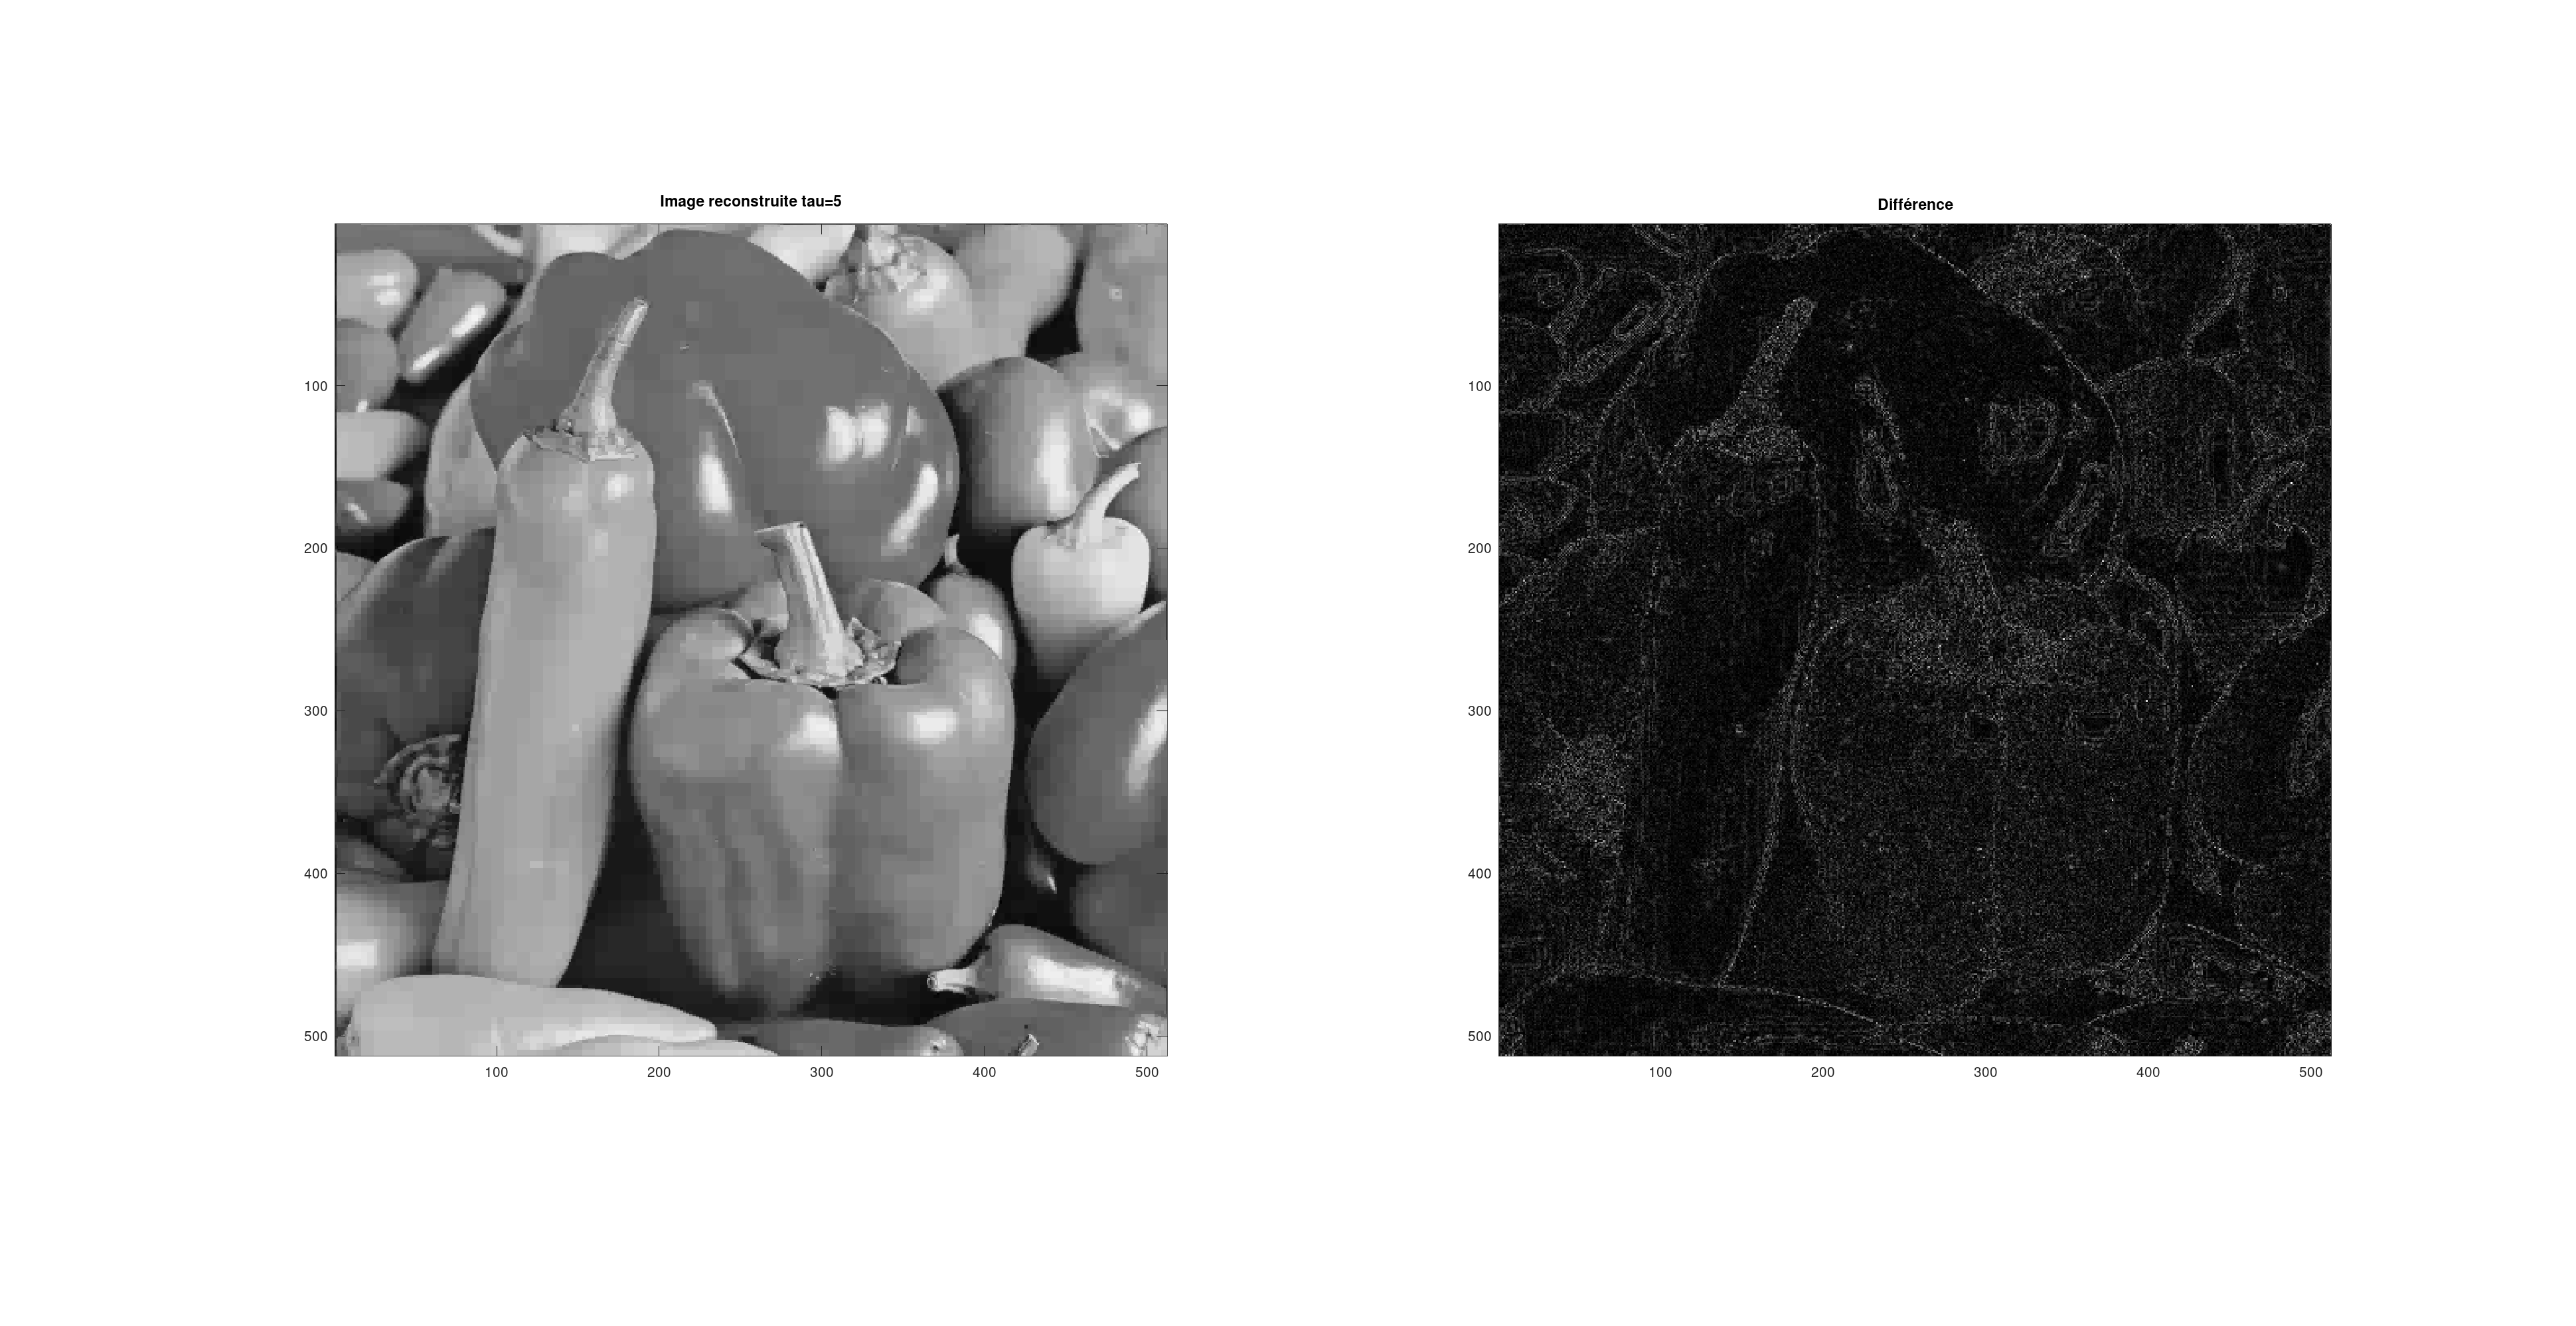
\includegraphics[width=\textwidth]{ex3_9}
                    \centering
                \end{figure}

                \begin{figure}[H]
                    \caption{Résultats pour $\tau = 20\%$}
                    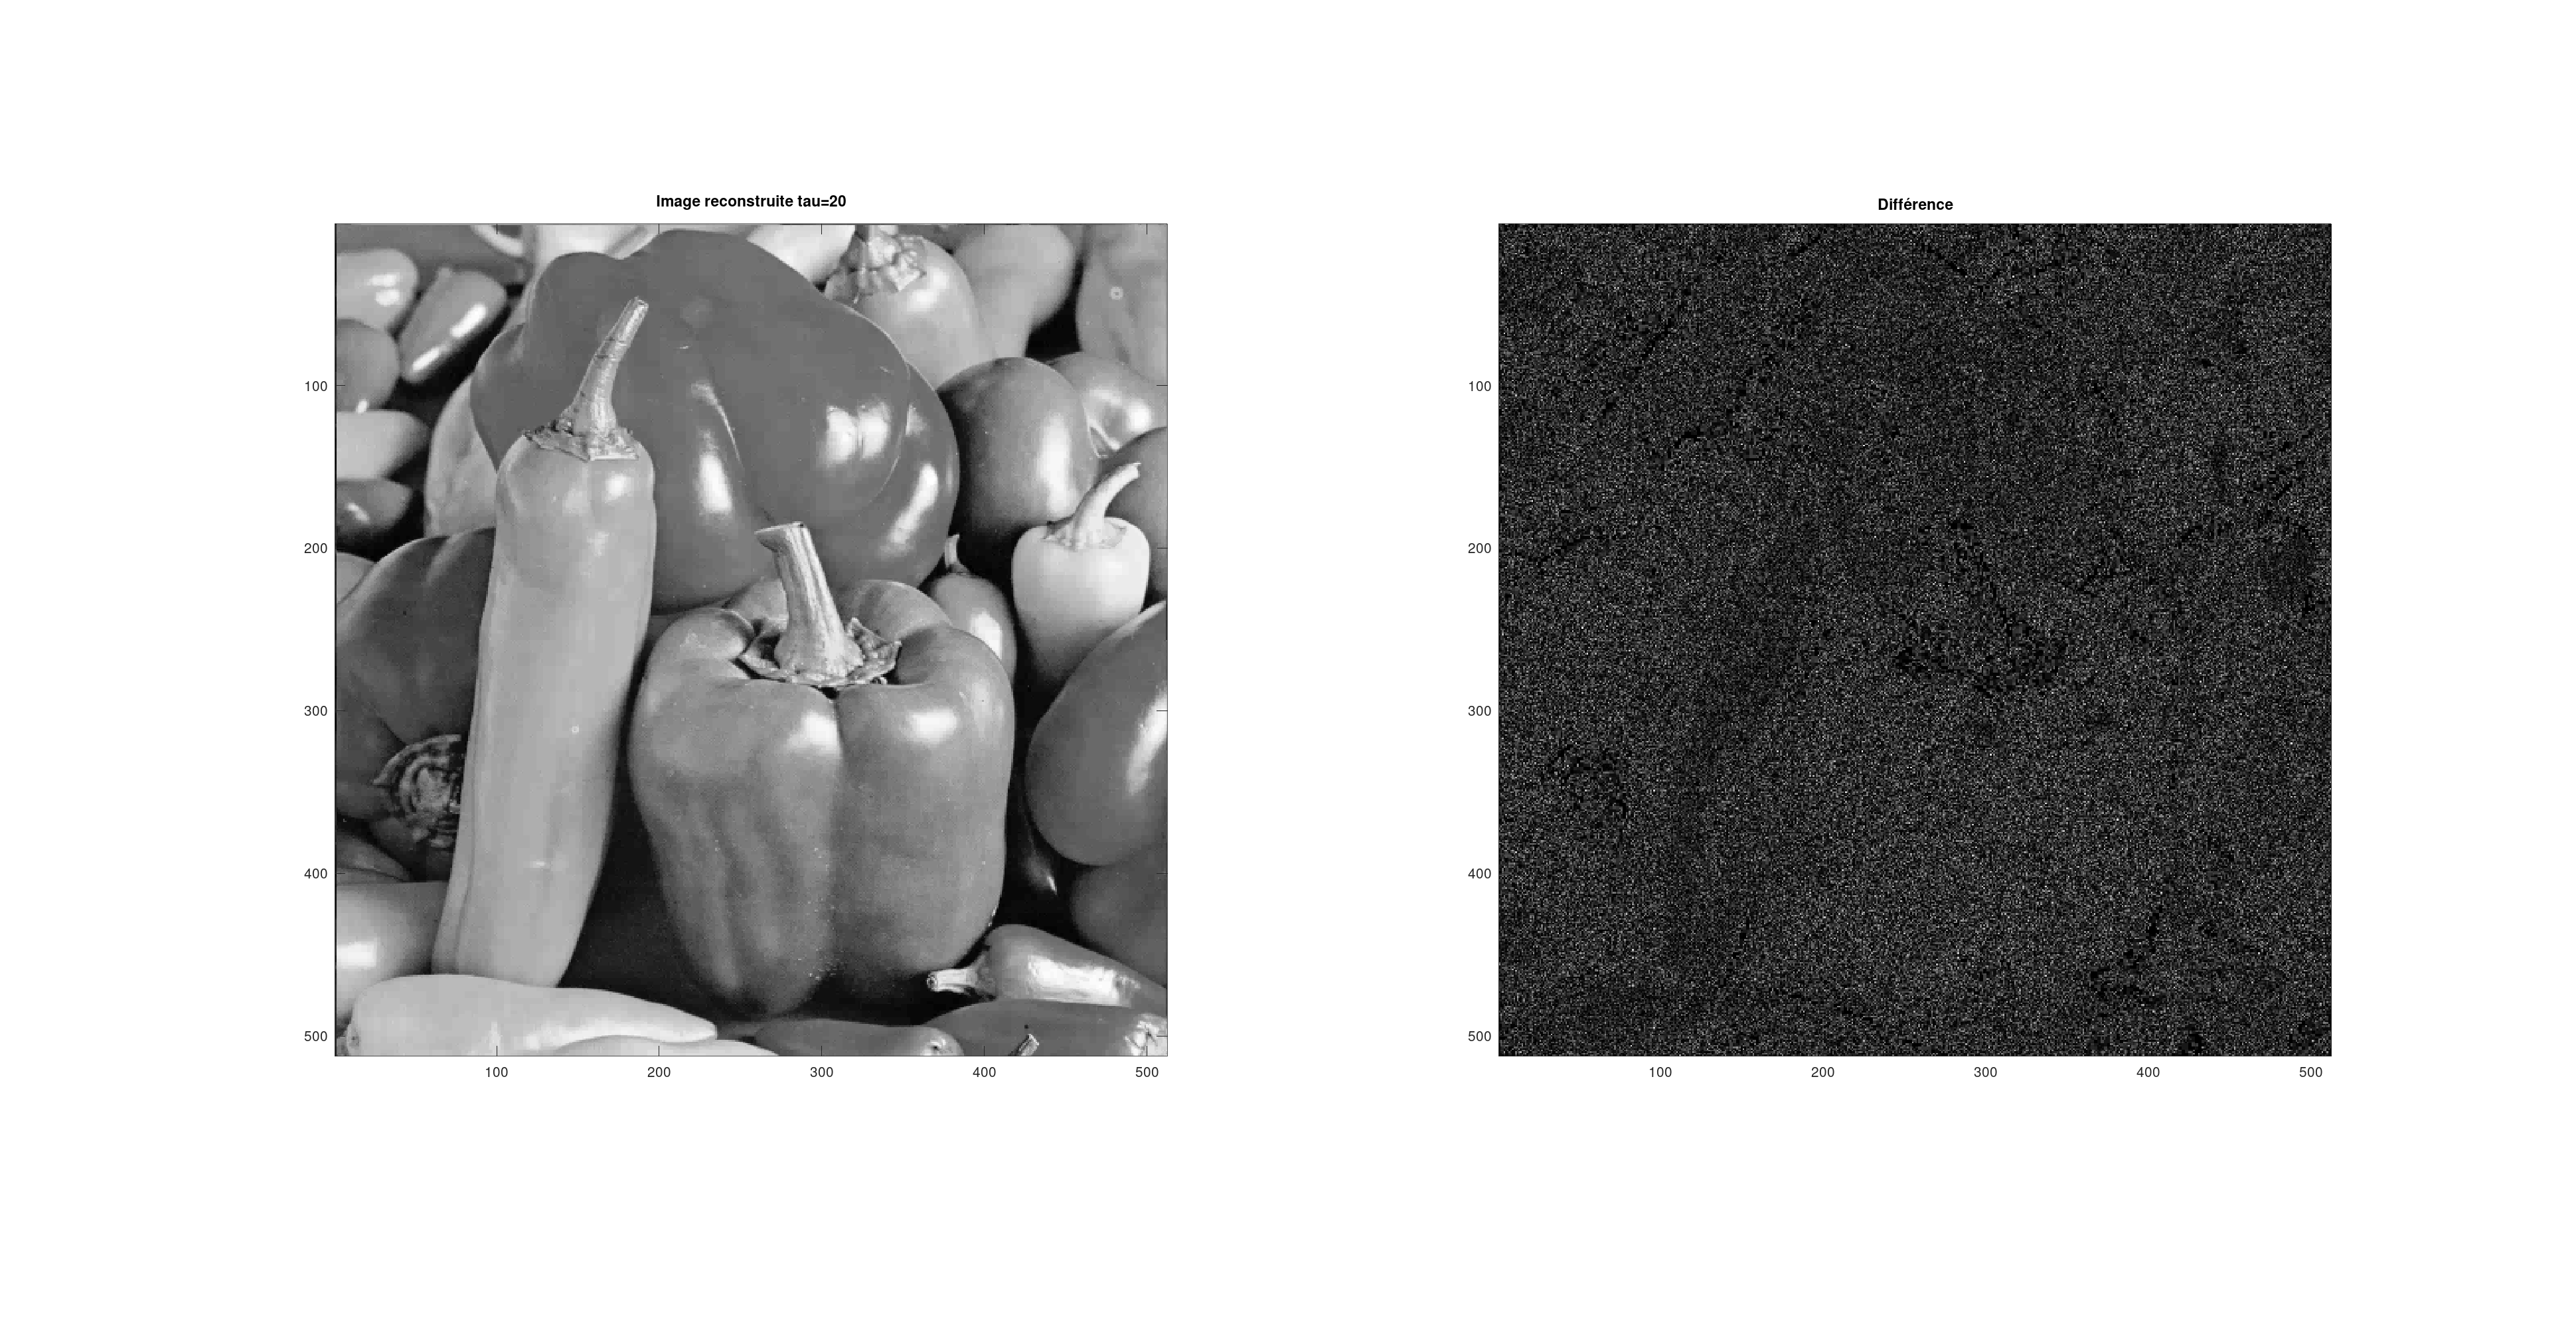
\includegraphics[width=\textwidth]{ex3_10}
                    \centering
                \end{figure}

            }

            On remarque alors que les résultats obtenus avec un filtre générateur de Daubechies
            do'rdre 4 les résultats sont meilleurs qu'avec une ondelette de Haar. En effet,
            l'image de différence dans le cas d'une ondelette de Haar est plus riche. On a ainsi
            annulé des coefficients correspondant à des informations utiles, il faut une valeur
            de $\tau$ plus élevée que pour le premier cas.

        \end{enumerate}

        \section*{Conclusion}

        Ainsi, la transformée en ondelettes discrète a plusieurs applications. Elle permet par
        exemple le débruitage de signaux ou la compression d'images. Ces applications reposent
        sur le fait que cette transformée laisse généralement place à plusieurs coefficients
        nuls. Nous avons aussi pu manipuler différents types d'ondelettes (Haar, Daubechies) et
        comprendre que pour chaque utilisation il convient de choisir attentivement l'ondelette
        afin d'obtenir de meilleurs résultats.

\end{enumerate}

\pagebreak

\begin{appendices}

    \section{Tracé d'ondelettes et de fonctions échelles par DWT inverse}

    \lstinputlisting[language=Matlab]{../ex1.m}

    \section{Débruitage dans l'espace des ondelettes}

    \lstinputlisting[language=Matlab]{../ex2.m}

    \section{Compression d'images}

    \lstinputlisting[language=Matlab]{../ex2.m}

\end{appendices}

\end{document}
